\chapter{Oscillation Analysis}
\label{chap:OscillationAnalysis}

The \texttt{MaCh3} framework used throughout this thesis has been validated through many tests. The code which handles the beam far detector seamples was validated by comparison to the 2020 T2K analysis. The sample event rates and log-likelihood scans generated by the framework used within this thesis were compared to those from the T2K analysis by the author of this thesis. Variations of the sample spectra were compared at \quickmath{\pm 1,3 \sigma} and good agreement was found in all cases. A similar study, led by Dr. C. Wret was used to validate the near detector portion of the code. The implementation of the atmospheric samples within \texttt{MaCh3} was cross-checked by the author of this thesis against the P-Theta framework. Both fitters are provided the same inputs and thus act as self-validation. These validations compared the event rate and log-likelihood scans. Documenation of all the above validations can be found in \cite{t2k_tn_426}.

\section{Monte Carlo Prediction}
\label{sec:OscillationAnalysis_MonteCarloPred}

Using the three sets of dial values defined in \autoref{sec:SelsAndSysts_Systs_Interaction}, the predicted event rates for each sample are defined in \autoref{tab:OscillationAnalysis_MCPred}. Both the oscillated event rates assuming Asimov A oscillation parameters (defined in \autoref{tab:Theory_ParameterSets}) and the un-oscillated event rates are given.

\begin{table}[ht!]
    \centering
    \begin{tabular}{|l|c|c|c|c|c|c|}
      \hline
      & \multicolumn{6}{|c|}{Total Predicted Events} \\
      \cline{2-7}
      & \multicolumn{2}{|c}{Generated} & \multicolumn{2}{|c}{Pre-fit} & \multicolumn{2}{|c|}{Post-fit} \\
      \cline{2-7}
      Sample & Osc & UnOsc & Osc & UnOsc & Osc & UnOsc \\
      \hline
      \texttt{SubGeV-elike-0dcy} & 7121.0 & 7102.6 & 6556.8 & 6540.0 & 7035.2 & 7015.7 \\
      \texttt{SubGeV-elike-1dcy} & 704.8 & 725.5 & 693.8 & 712.8 & 565.7 & 586.0 \\
      \texttt{SubGeV-mulike-0dcy} & 1176.5 & 1737.2 & 1078.6 & 1588.1 & 1182.7 & 1757.1 \\
      \texttt{SubGeV-mulike-1dcy} & 5850.7 & 8978.1 & 5351.7 & 8205.1 & 5867.0 & 9009.9 \\
      \texttt{SubGeV-mulike-2dcy} & 446.9 & 655.2 & 441.6 & 647.7 & 345.9 & 505.6 \\
      \texttt{SubGeV-pi0like} & 1438.8 & 1445.4 & 1454.9 & 1461.1 & 1131.1 & 1136.2 \\
      \texttt{MultiGeV-elike-nue} & 201.4 & 195.6 & 201.1 & 195.3 & 202.6 & 196.7 \\
      \texttt{MultiGeV-elike-nuebar} & 1141.5 & 1118.3 & 1060.7 & 1039.5 & 1118.5 & 1095.7 \\
      \texttt{MultiGeV-mulike} & 1036.7 & 1435.8 & 963.1 & 1334.1 & 1015.2 & 1405.9 \\
      \texttt{MultiRing-elike-nue} & 1025.1 & 982.2 & 1026.8 & 984.3 & 1029.8 & 986.4 \\
      \texttt{MultiRing-elike-nuebar} & 1014.8 & 984.5 & 991.0 & 962.0 & 1008.9 & 978.5 \\
      \texttt{MultiRing-mulike} & 2510.0 & 3474.4 & 2475.6 & 3425.8 & 2514.6 & 3480.4 \\      
      \texttt{MultiRingOther-1} & 1204.5 & 1279.1 & 1205.8 & 1280.3 & 1207.4 & 1281.0 \\
      \texttt{PCStop} & 349.2 & 459.2 & 338.4 & 444.7 & 346.8 & 456.1 \\
      \texttt{PCThru} & 1692.8 & 2192.5 & 1661.5 & 2149.8 & 1689.2 & 2187.8 \\
      \texttt{UpStop-mu} & 751.2 & 1295.0 & 739.7 & 1271.6 & 750.4 & 1293.0 \\
      \texttt{UpThruNonShower-mu} & 2584.4 & 3031.6 & 2577.9 & 3019.4 & 2586.8 & 3034.0 \\
      \texttt{UpThruShower-mu} & 473.0 & 488.6 & 473.2 & 488.7 & 473.8 & 489.4 \\
      \texttt{FHC1Rmu} & 328.0 & 1409.2 & 301.1 & 1274.7 & 345.1 & 1568.0 \\
      \texttt{RHC1Rmu} & 133.0 & 432.3 & 122.7 & 396.2 & 135.0 & 443.9 \\
      \texttt{FHC1Re} & 84.6 & 19.2 & 77.4 & 18.2 & 93.7 & 19.7 \\
      \texttt{RHC1Re} & 15.7 & 6.4 & 14.6 & 6.1 & 15.9 & 6.3 \\
      \texttt{FHC1Re1de} & 10.5 & 3.2 & 10.3 & 3.1 & 8.8 & 2.9 \\
      \hline
      \hline
    \end{tabular}
    \caption{The Monte Carlo prediction of each sample observed at SK used within this analysis. Three model parameter tunes are considered, as defined in \autoref{sec:SelsAndSysts_Systs_Interaction}. The oscillated predictions assumed Asimov A oscillation parameters provided in \autoref{tab:Theory_ParameterSets}.}
    \label{tab:OscillationAnalysis_MCPred}
\end{table}

Generally, samples which target CCQE interaction modes observe a decrease in prediction when using the pre-fit dial values. This is in accordance with the Monte Carlo being produced assumed \quickmath{M_{A}^{QE} = 1.21\text{GeV}} whilst the pre-fit dial value should be \quickmath{M_{A}^{QE} = 1.03\text{GeV}}, as suggested by \cite{t2k_tn_344}. Furthermore, the predicted event rates of samples which target CCRES interaction modes is significantly reduced when considering the post-ND fit. This follows the observations in \autoref{sec:SelsAndSysts_Systs_Interaction}. The strength of the accelerator neutrino experiment can also be seen in the remarkable difference between the oscillated and unoscillated predictions in the \texttt{FHC1Rmu} and \texttt{RHC1Rmu} samples. There is a very obvious decrease in the expected event rate between the two predictions which is not as clearly observed in the atmospheric samples. This is due to the fact that the beam energy is tuned to the maximum disappearance probability, which is not the case for the naturally generated atmospheric neutrinos.

\section{Likelihood Calculation}
\label{sec:OscillationAnalysis_LLHCalc}

This analysis performs a joint oscillation parameter fit of the ND280,  and the SK atmospheric samples.

Once the Monte Carlo predictions of each beam and atmospheric sample has been built, following from \autoref{chap:SelsAndSysts}, a likelihood needs to be constructed. This is done by comparing the Monte Carlo prediction to ``data''. The data can consist of either an Asmiov Monte Carlo prediction, which is typically used for sensitivity studies, or real data. The Monte Carlo prediction is calculated at a particular point, \quickmath{\vec{\theta}}, in the model parameter space, \quickmath{N_{i}^{MC} = N_{i}^{MC}(\vec{\theta})}. Both the data and Monte Carlo spectra are binned, where the \quickmath{i^{th}} bin content is represented by \quickmath{N_{i}^{D}} and \quickmath{N_{i}^{MC}}, respectively. The bin contents for the beam near detector, beam far detector and atmospheric samples are denoted with \quickmath{ND}, \quickmath{FD} and \quickmath{Atm}, respectively. The binning index, \quickmath{i}, runs over all the bins within the sample and all samples with that set. Taking the beam far detector samples as example, it would run over all the reconstructed neutrino energy bins in all samples (FHC\quickmath{1\text{R}\mu}, RHC\quickmath{1\text{R}\mu}, etc.). The likelihood calculation between data and Monte Carlo for a particular bin follows a Poisson distribution, where the data is treated as a fluctuation of the simulation. 

Following the T2K analysis presented in \cite{Dunne2020-uf}, the likelihood contribution from the near detector also includes a Monte Carlo statistical uncertainty term, derived from the Barlow and Beeston statistical treatment \cite{Barlow1993-cc, Conway2011-go}. In addition to treating the data as a fluctuation of the Monte Carlo prediction, it includes a contribution from the likelihood that the generated simulation is a statistical fluctuation of the actual true simulation assuming infinite statistics. The technical implementation of this additional likelihood term is documented in \cite{t2k_tn_395}. The term is defined as,

\begin{equation}
  \frac{(\beta_{i}-1)^{2}}{2\sigma^{2}_{\beta_{i}}},
\end{equation}

where \quickmath{\beta_{i}} represents a scaling parameter for each bin \quickmath{i}, which is a value based on the amount of Monte Carlo statistics in a bin \cite{t2k_tn_395}. \quickmath{\sigma_{\beta_{i}} = \sqrt{\sum_{i} w_{i}^{2}}/N_{i}^{MC}}, and \quickmath{\sqrt{\sum_{i} w_{i}^{2}}} represents the sum of the square of the weights of the Monte Carlo events which fall into bin \quickmath{i}.

Additional contributions to the likelihood come from the variation of the systematic model parameters. For those parameters with well-motivated uncertainty estimates, a covariance matrix, \quickmath{V} describes the prior knowledge of each parameter as well as any correlations between the parameters. Due to the technical implementation, a single covariance matrix describes each ``block'' of model parameters, e.g. beam flux systematics. For simplicity, the covariance matrix associated with the \quickmath{k^{th}} block is denoted \quickmath{V^{k}}. This substitution results in \quickmath{\vec{\theta} = \sum_{k}^{N_{b}} \vec{\theta}^{k}} and \quickmath{V = \sum_{k}^{N_{b}} V^{k}}, for \quickmath{N_{b}} number of blocks describing: oscillation parameters, beam flux, atmospheric flux, neutrino interaction, near detector, beam far detector and atmospheric far detector systematics detailed in \autoref{sec:SelsAndSysts_Systs}. The number of parameters in the \quickmath{k^{th}} block is defined as \quickmath{n(k)}.

The final likelihood term is defined as,

\begin{align}
\label{eqn:Likelihood:Likelihood}
&-\ln(\mathcal{L}) = \\ 
& \sum_{i}^{\mathsf{ND bins}} N_{i}^{\mathrm{ND},MC}(\vec{\theta}) - N_{i}^{\mathrm{ND},D} + N_{i}^{\mathrm{ND},D}  \times \ln \left[ N_{i}^{\mathrm{ND},D}/N_{i}^{\mathrm{ND},MC}(\vec{\theta}) \right] + \frac{(\beta_{i}-1)^{2}}{2\sigma^{2}_{\beta_{i}}} \nonumber \\
& +  \sum_{i}^{\mathsf{FD bins}} N_{i}^{\mathrm{FD},MC}(\vec{\theta}) - N_{i}^{\mathrm{FD},D} + N_{i}^{\mathrm{FD},D}  \times \ln \left[ N_{i}^{\mathrm{FD},D}/N_{i}^{\mathrm{FD},MC}(\vec{\theta}) \right] \nonumber \\ 
& +  \sum_{i}^{\mathsf{Atm bins}} N_{i}^{\mathrm{Atm},MC}( \vec{\theta}) - N_{i}^{\mathrm{Atm},D} + N_{i}^{\mathrm{Atm},D} \times  \ln \left[ N_{i}^{\mathrm{Atm},D}/N_{i}^{\mathrm{Atm},MC}(\vec{\theta}) \right] \nonumber \\ 
& + \frac{1}{2} \sum_{k}^{N_{b}} \sum_{i}^{n(k)} \sum_{j}^{n(k)} (\vec{\theta}^{k})_{i} (V^{k})^{-1}_{ij} (\vec{\theta}^{k})_{j}. \nonumber
\end{align}

This is the value determined at each step of the MCMC to build the posterior distribution, as discussed in \autoref{chap:MarkovChainMonteCarlo}.

\subsection{Likelihood Scans}
\label{sec:OscillationAnalysis_LLHScans}

Using the defintion of the likelihood presented in \autoref{sec:OscillationAnalysis_LLHCalc}, the response of each sample to a variation particular parameter can be studied. \autoref{fig:OscillationAnalysis_LLHScanOscPars} presents the variation of all the samples (beam and atmospheric) at SK. Each plot represents a ``scan'', where a particular parameter is scanned in some range. The ``data'' being used within the definition of the likelihood equation is built using the Asimov A oscillation parameter values defined in \autoref{tab:Theory_ParameterSets} alongside the pre-fit dial values as discussed in \autoref{sec:SelsAndSysts_Systs_Interaction}. Due to the caveat of fixed systematic parameters and correlations between oscillation parameters being ignored within these likelihood scans, the value of \quickmath{\chi^{2} \sim 1} does not equate to the typical \quickmath{1\sigma} sensitivity. However, it does give an indication of which samples response the strongest to a variation in the oscillation parameters. The point at which the likelihood tends to zero illustrates the value of the parameter used to build the Asimov data prediction. The likelihood scans only include the sample response and ignore the penalty contribution term from the variation of the parameter.

\begin{figure}[h]
  \begin{subfigure}[t]{0.5\textwidth}
    \includegraphics[width=\textwidth, trim={0mm 0mm 0mm 0mm}, clip,page=4]{Figures/OA/LLHScans_Osc.pdf}
    \subcaption{\quickmath{\sin^{2}(\theta_{23})}}
  \end{subfigure}%
  \begin{subfigure}[t]{0.5\textwidth}
    \includegraphics[width=\textwidth, trim={0mm 0mm 0mm 0mm}, clip,page=7]{Figures/OA/LLHScans_Osc.pdf}
    \subcaption{\quickmath{\Delta m^{2}_{23}}}
  \end{subfigure}
  \begin{subfigure}[t]{0.5\textwidth}
    \includegraphics[width=\textwidth, trim={0mm 0mm 0mm 0mm}, clip,page=8]{Figures/OA/LLHScans_Osc.pdf}
    \subcaption{\quickmath{\delta_{CP}}}
  \end{subfigure}%
  \begin{subfigure}[t]{0.5\textwidth}
    \includegraphics[width=\textwidth, trim={0mm 0mm 0mm 0mm}, clip,page=5]{Figures/OA/LLHScans_Osc.pdf}
    \subcaption{\quickmath{\sin^{2}(\theta_{13})}}
  \end{subfigure}
  \begin{subfigure}[t]{0.5\textwidth}
    \includegraphics[width=\textwidth, trim={0mm 0mm 0mm 0mm}, clip,page=3]{Figures/OA/LLHScans_Osc.pdf}
  \end{subfigure}
  \caption{The response of the likelihood, as defined in \autoref{sec:OscillationAnalysis_LLHCalc}, illustrating the response of the samples to the oscillation parameters. \delmsqsol and \sinsqsol are negated because these samples have no sensitivity to those parameters. The Asimov data set is built using the pre-fit dial values assuming Asimov A oscillation parameters defined in \autoref{tab:Theory_ParameterSets}.}
  \label{fig:OscillationAnalysis_LLHScanOscPars}
\end{figure}

The sensitivity to \sinsqatm is mostly dominated by the beam samples although the atmospheric sample contribution is certainly non-negligble. The summed response over all atmospheric samples becomes comparable to that of the muon-like beam samples. Consequently, one would expect that the joint fit would become more sensivity to \sinsqatm than just T2K experiment alone. For this particular choice of asimov point, the only samples which respond to the \sinsqreac parameter are the electron-like beam samples. Consequently, no increase in sensitivity beyond that of the T2K-only analysis is expected. Furthermore, the sensitivity of the beam sample is significantly weaker than the reactor constraint so the `reactor constraint' prior will dominate any measurement it is included within. The \delmsqsol and \sinsqsol are not considered as there is simply no sensitivity in any sample considered within this analysis. The response to \delmsqatm is much larger in beam samples, specfically for the \quickmath{\mu}-like samples, compared to atmospheric samples. This is to be expected as the beam neutrino energy can be specifically tuned to match the maximal disappearance probability. %As discussed in \autoref{sec:Oscillation_Overview}, the determination of the mass hierarchy is signficantly enhanced when using the atmospheric samples due to them transitioning through the Earth's core. So whilst the atmospheric samples do not add much information to the constraint of \quickmath{|\Delta m^{2}_{32}|} beyond that of the beam analysis, they do enhance the ability to determine the sign of the parameter.
  
The correlations between oscillation parameters induce marignalisation effects within the response of the likelihood. That is to say, the response to \dcp is affected by the choice of \sinsqreac or \sinsqatm. The two-dimensional scans of the appearance (\sinsqreac-\dcp) and disappearance (\sinsqatm-\delmsqatm) parameters are illustrated in \autoref{fig:OscillationAnalysis_2DLLHOscScans_App} and \autoref{fig:OscillationAnalysis_2DLLHOscScans_Dis}, respectively. The caveat of fixed systematic parameters and correlations between other oscillation parameters being neglected still apply.

The appearance log-likelihood scans show the distinct difference in how the beam and atmospheric samples respond. The beam samples have an approximately constant width of the \quickmath{2\sigma} and \quickmath{3\sigma} contours, throughout all ranges of \dcp. The atmospheric samples response to \dcp is very strongly correlated to the choice of \sinsqreac, with the strongest constraints around \quickmath{\delta_{CP}\sim1}. Consequently, this difference allows some of the degeneracy in a beam-only fit to be broken. Comparing the beam and joint fit log-likelihood scans, the \quickmath{2\sigma} continous contour in \dcp for beam samples is broken when the atmospheric samples are added. Furthermore, the width of the \quickmath{3\sigma} contours also becomes dependent upon the value of \dcp. Whilst these are encouraging results for the joint fit, these are not sensitivity measurements as the systematic parameters are fixed and the correlation between oscillation parameters is neglected.

The disappearance log-likelihood scans in \sinsqatm-\delmsqatm space show the expected result when considering the one-dimensional scans already discussed. The uncertainty on the width of \quickmath{|\Delta m^{2}_{32}|} is mostly driven by the beam-only sensitivties. However, the width of this contour in the inverted mass region (\quickmath{\Delta m^{2}_{32} < 0}) is significantly reduced due to the ablity of the atmospheric samples to select the correct mass hierarchy (these log-likelihood scans use the Asimov A oscillation probabilities which assumes true normal hierarchy). The width of the uncertainty in \sinsqatm is also reduce compared to a beam-only analysis, with a further decrease in the inverted hierarchy region due to mass hierarchy determination.

\begin{figure}[h]
  \begin{subfigure}[t]{0.5\textwidth}
    \subcaption{Beam Samples}
    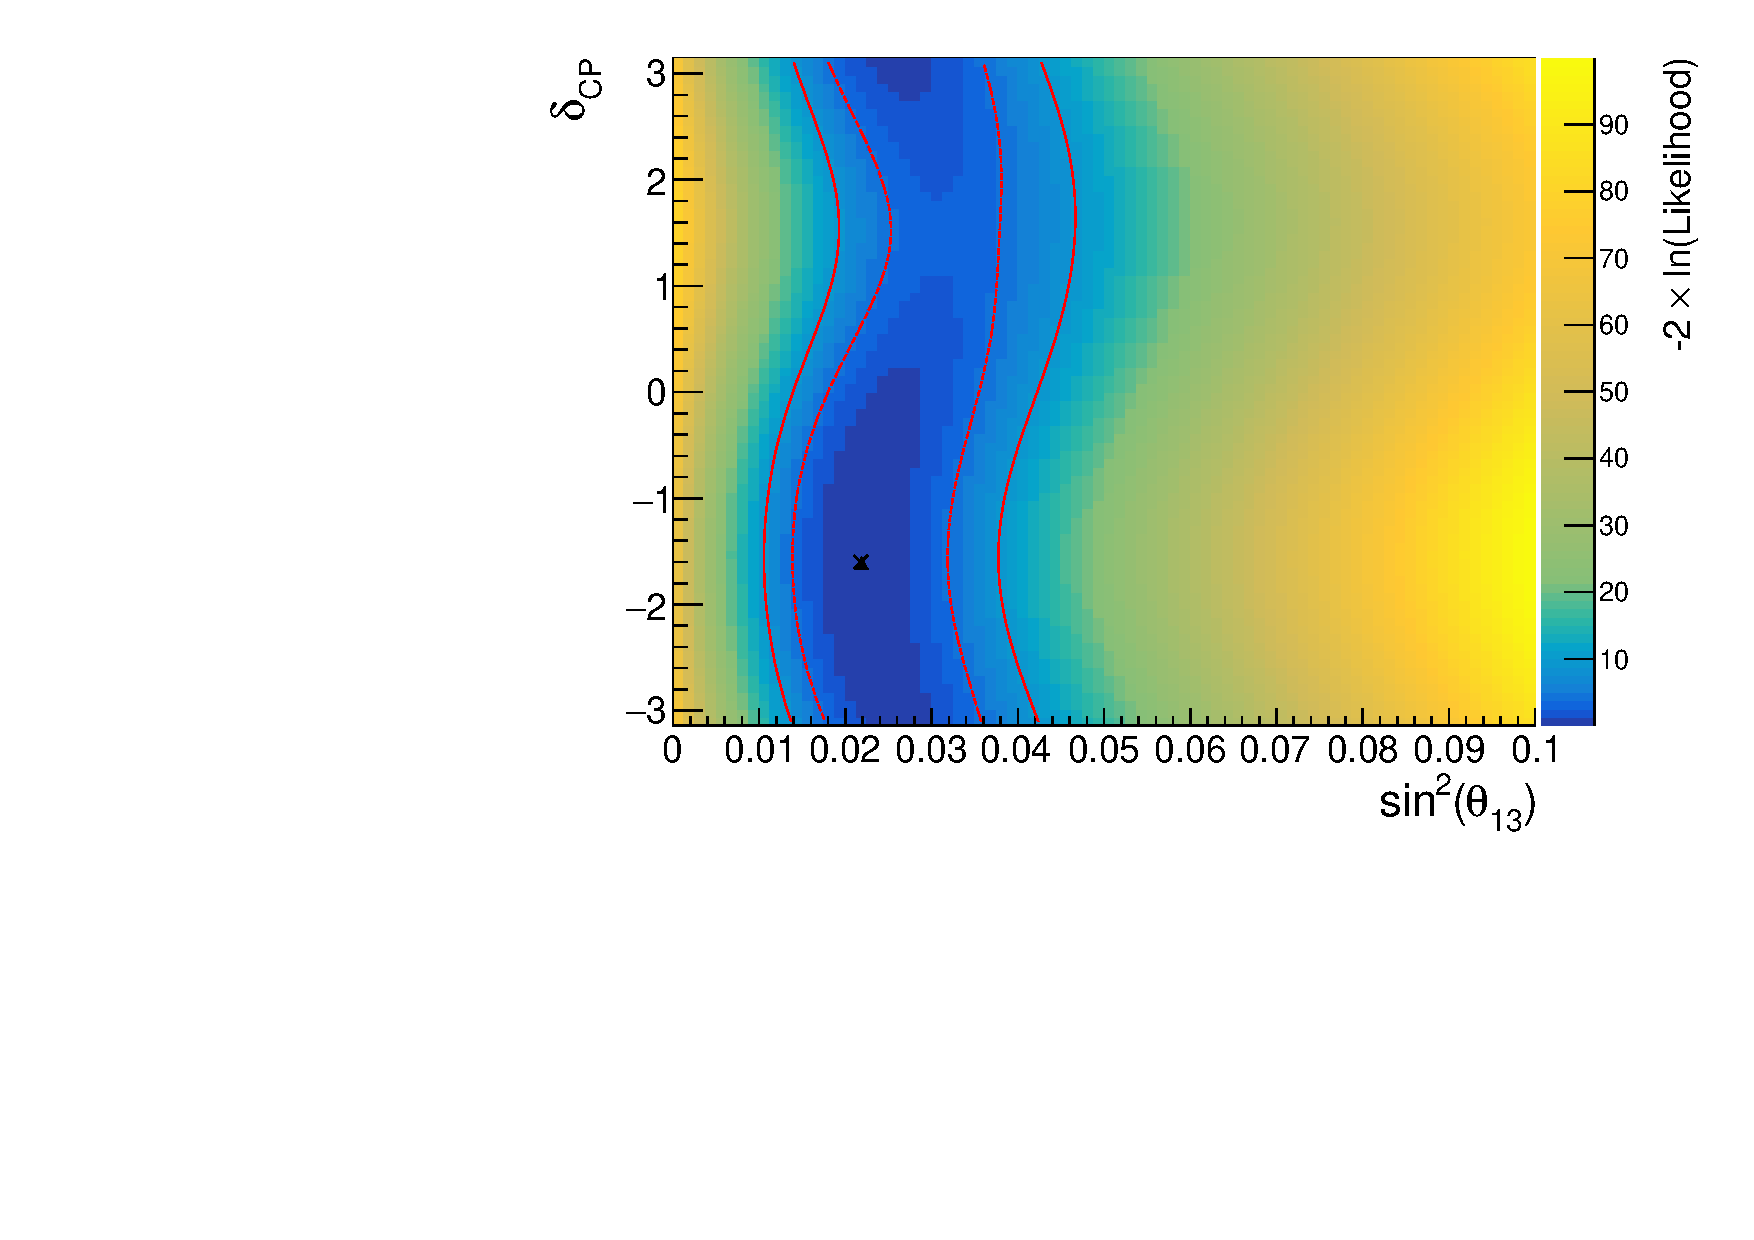
\includegraphics[width=\textwidth, trim={0mm 0mm 0mm 0mm}, clip,page=1]{Figures/OA/AppearanceScans.pdf}
  \end{subfigure}%
  \begin{subfigure}[t]{0.5\textwidth}
    \subcaption{Atmospheric Samples}
    \includegraphics[width=\textwidth, trim={0mm 0mm 0mm 0mm}, clip,page=2]{Figures/OA/AppearanceScans.pdf}
  \end{subfigure}
  \begin{subfigure}[t]{1.0\textwidth}
    \subcaption{All Samples}
    \includegraphics[width=\textwidth, trim={0mm 0mm 0mm 0mm}, clip,page=3]{Figures/OA/AppearanceScans.pdf}
  \end{subfigure}
  \caption{Two-dimensional log-likelihood scan of the appearance (\sinsqreac-\dcp) parameters showing the response of the beam samples (top), atmospheric samples (middle) and the summed response (bottom). The Asimov A oscillation parameters, defined in \autoref{tab:Theory_ParameterSets}, are assumed to be the true point (Black Cross). The position of the smallest log-likelihood is highlighted with the triangle. Prior uncertainty terms of the oscillation parameters are neglected. The two(three) sigma contour levels are illlustrated with the dashed(solid) red line.}
  \label{fig:OscillationAnalysis_2DLLHOscScans_App}
\end{figure}

\begin{figure}[h]
  \begin{subfigure}[t]{0.5\textwidth}
    \subcaption{Beam Samples}
    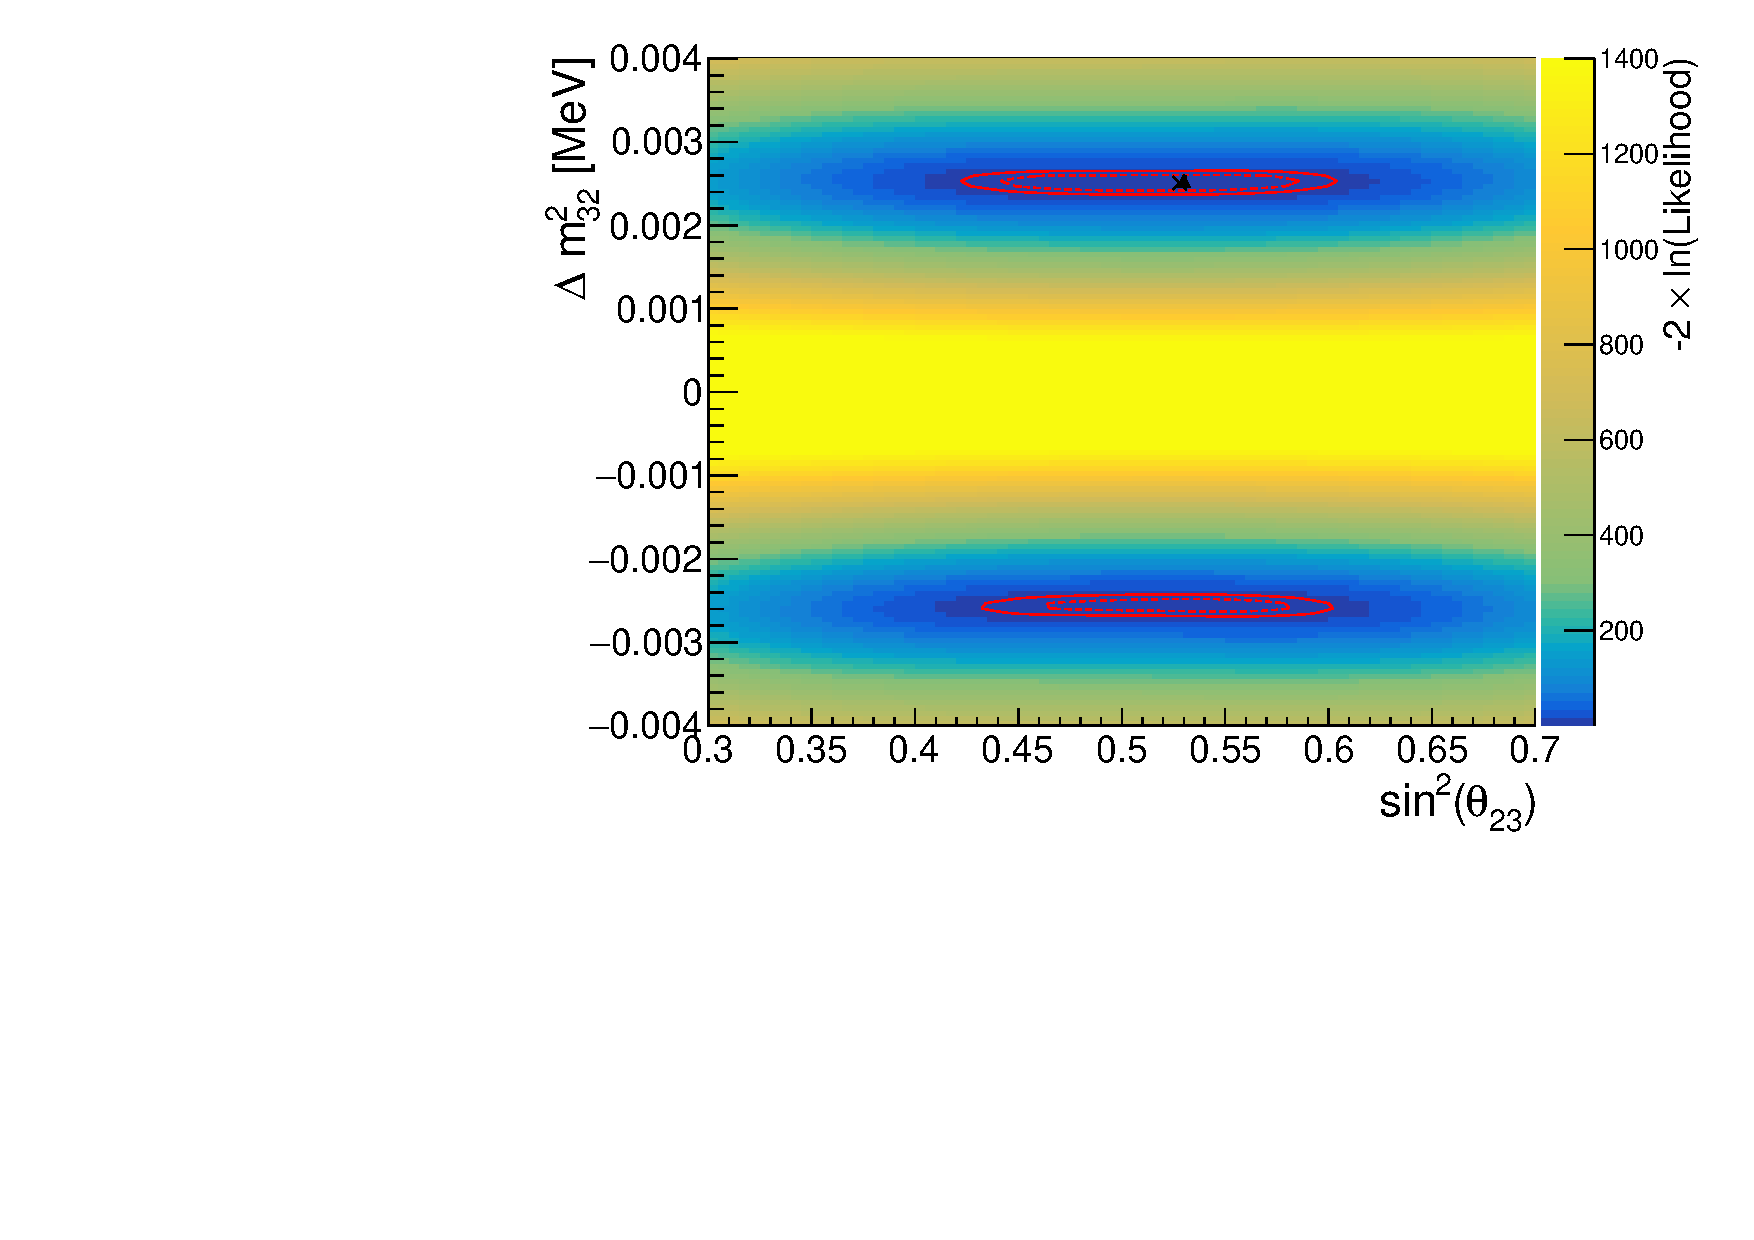
\includegraphics[width=\textwidth, trim={0mm 0mm 0mm 0mm}, clip,page=1]{Figures/OA/DisappearanceScans.pdf}
  \end{subfigure}%
  \begin{subfigure}[t]{0.5\textwidth}
    \subcaption{Atmospheric Samples}
    \includegraphics[width=\textwidth, trim={0mm 0mm 0mm 0mm}, clip,page=2]{Figures/OA/DisappearanceScans.pdf}
  \end{subfigure}
  \begin{subfigure}[t]{1.0\textwidth}
    \subcaption{All Samples}
    \includegraphics[width=\textwidth, trim={0mm 0mm 0mm 0mm}, clip,page=3]{Figures/OA/DisappearanceScans.pdf}
  \end{subfigure}
  \caption{Two-dimensional log-likelihood scan of the disappearance (\sinsqatm-\delmsqatm) parameters showing the response of the beam samples (top), atmospheric samples (middle) and the summed response (bottom). The Asimov A oscillation parameters, defined in \autoref{tab:Theory_ParameterSets}, are assumed to be the true point (Black Cross). The position of the smallest log-likelihood is highlighted with the triangle. Prior uncertainty terms of the oscillation parameters are neglected. The two(three) sigma contour levels are illlustrated with the dashed(solid) red line.}
  \label{fig:OscillationAnalysis_2DLLHOscScans_Dis}
\end{figure}

The log-likelihood scans illustrated thus far only give the sensitivity of this analysis at a fixed asimov point, namely Asimov A defined in \autoref{tab:Theory_ParameterSets}. Whilst computational infeasible to run many fits at different asimov points, it is possible to calculate the log-likelihood response to different asimov data sets. \autoref{fig:OscillationAnalysis_AsimovEval_DCP} and \autoref{fig:OscillationAnalysis_AsimovEval_TH23} illustrate how the sensitivity changes for differing values of \dcp and \sinsqatm, respectively, whilst the other oscillation parameters are fixed at Asimov A. Consequentally, the caveat of fixed systematic parameters and correlations between other oscillation parameters being neglected still applies.

To explain how these plots are made, consider \autoref{fig:OscillationAnalysis_AsimovEval_DCP}. This plot is built by considering multiple one-dimensional log-likelihood scans, each using the Asimov A oscillation parameter set but having a slightly differing value of \dcp. Consequently, the results can be interpretted as vertical slices of the log-likelihood response made at different asimov points. The procedure starts by building an asimov `data' prediction for a particular value of \dcp taken from the x-axis. Then a likelihood value is calculated at every \dcp point taken from the y-axis. This is then repeated for each point on the x-axis, such that a series of one dimensional likelihood scans are displayed in sequential order of \dcp.

\autoref{fig:OscillationAnalysis_AsimovEval_DCP} illustrates how the sensitivity to \dcp is offset between the beam and atmospheric samples. This offset agrees with the one dimensional scan illustrated in \autoref{fig:OscillationAnalysis_LLHScanOscPars}. Notably for the \quickmath{1\sigma} intervals, there are regions in the off-diagonal for which the beam and atmospheric samples have broken and discontinous contours. For example, for the asimov point \quickmath{\delta_{CP} = 0.}, the beam samples sensitivity would include two discontinous regions which would be preferred: \quickmath{\delta_{CP} = 0, \pi}. However the offset in \dcp between these beam and atmospheric samples allow the joint fit to have increased sensitivity in these regions, thus mitigating the degeneracy. However, the \quickmath{2\sigma} intervals from the joint fit are more similar to the two independent sensitivities and the off-diagonal degeneracies mostly remain. This indicates that the joint fit has the strength to aide parameter determination but still can not entirely break the degenearcies in \dcp at higher confidence levels. 

\autoref{fig:OscillationAnalysis_AsimovEval_TH23} illustrates the same study as above, although the value of \dcp is fixed to the Asimov A parameter set whilst the value of \sinsqatm is varied. Due to the beam parameters and baseline being tuned to specifically target this oscillation parameter, the average sensitivity of the beam samples is stronger than the atmospheric samples. However, the degeneracy around maximal mixing (\quickmath{\sin^{2}(\theta_{23} = 0.5)}) is significantly more peaked in the beam samples compared to the atmospheric samples. This behaviour is strengthened when considering the \quickmath{2\sigma} intervals, to the point where two distinct discontinous regions of the \quickmath{2\sigma} intervals exist around the asimov point \quickmath{\sin^{2}(\theta_{23}) \sim 0.41, 0.6}. Given the caveat of only considering log-likelihood scans, the joint analysis would mostly eliminate the discontinous intevals in these regions.

\begin{figure}[h]
  \begin{subfigure}[t]{1.0\textwidth}
    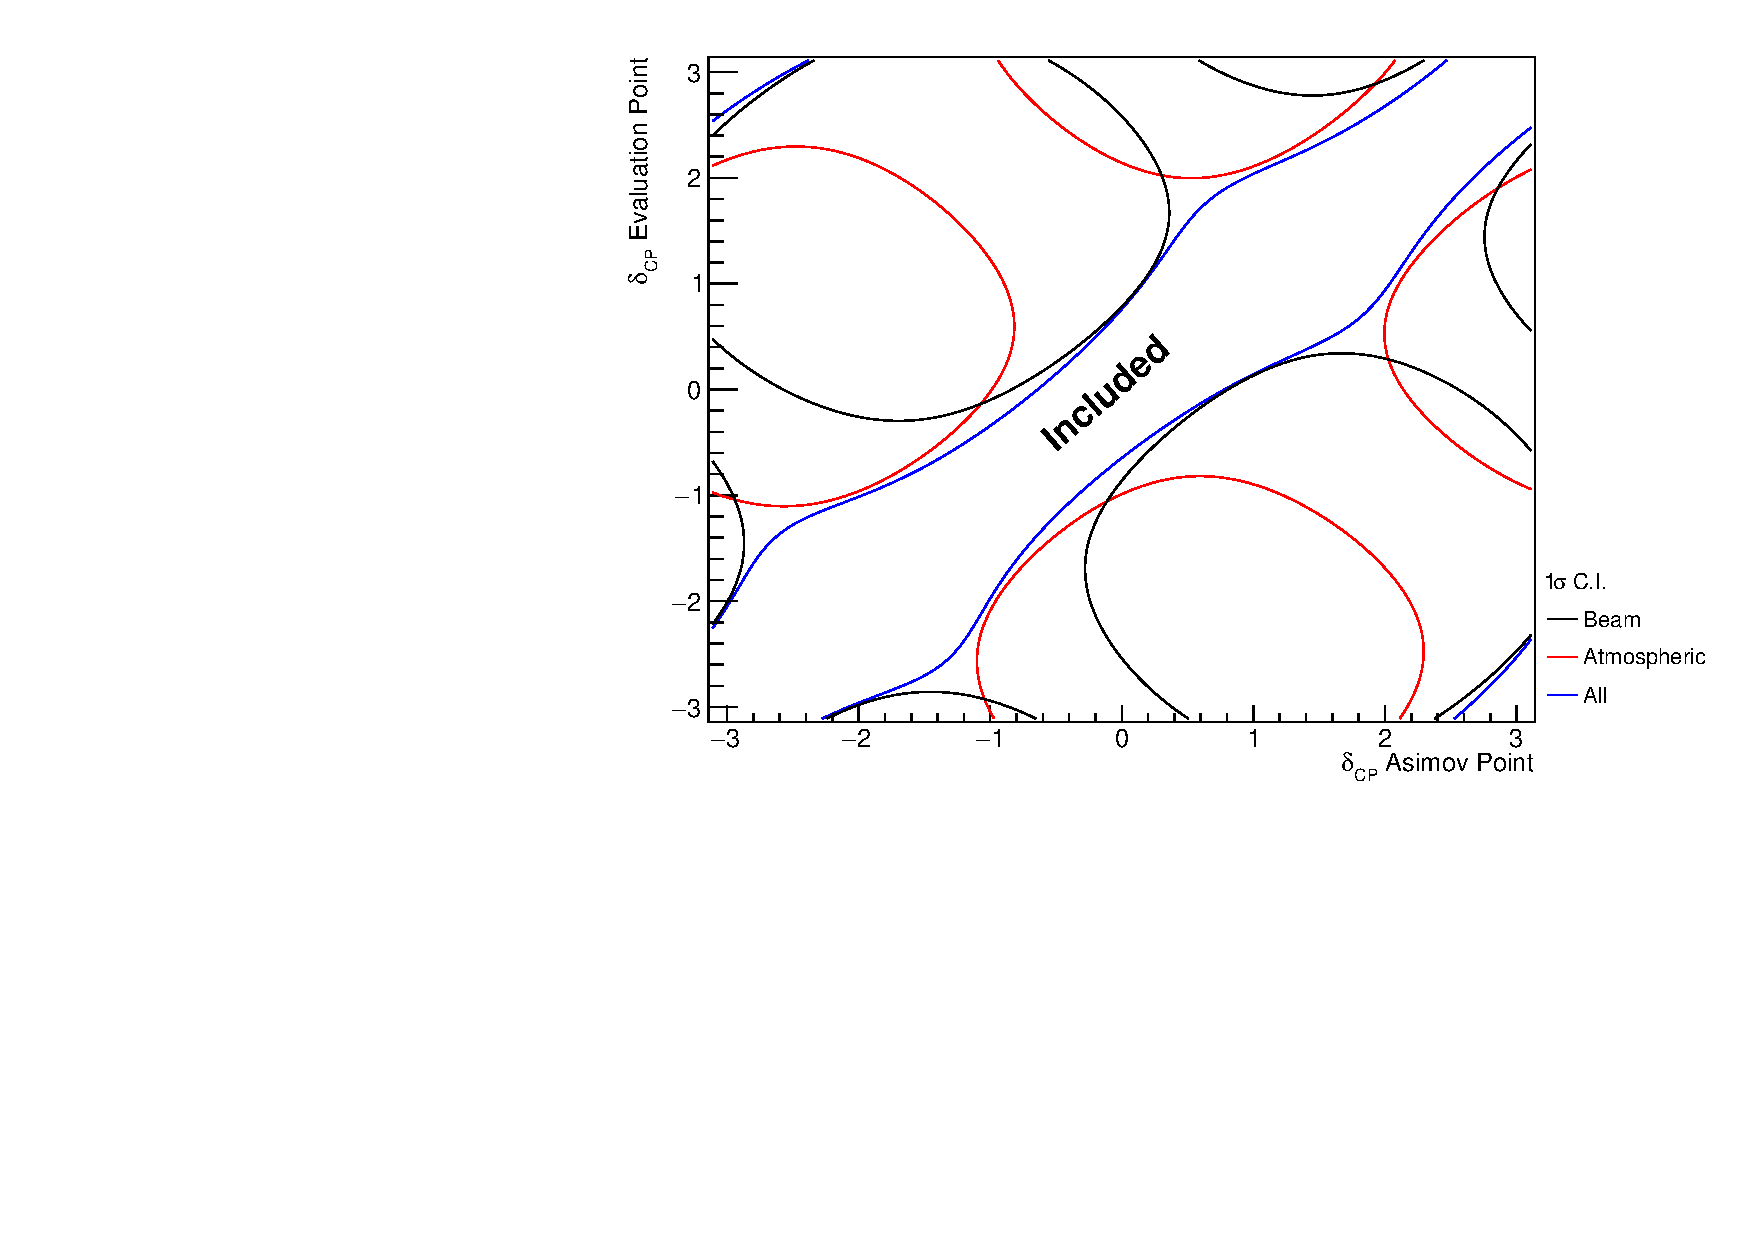
\includegraphics[width=\textwidth, trim={0mm 0mm 0mm 0mm}, clip,page=1]{Figures/OA/DCP_Scans_1Sig.pdf}
  \end{subfigure}
  \begin{subfigure}[t]{1.0\textwidth}
    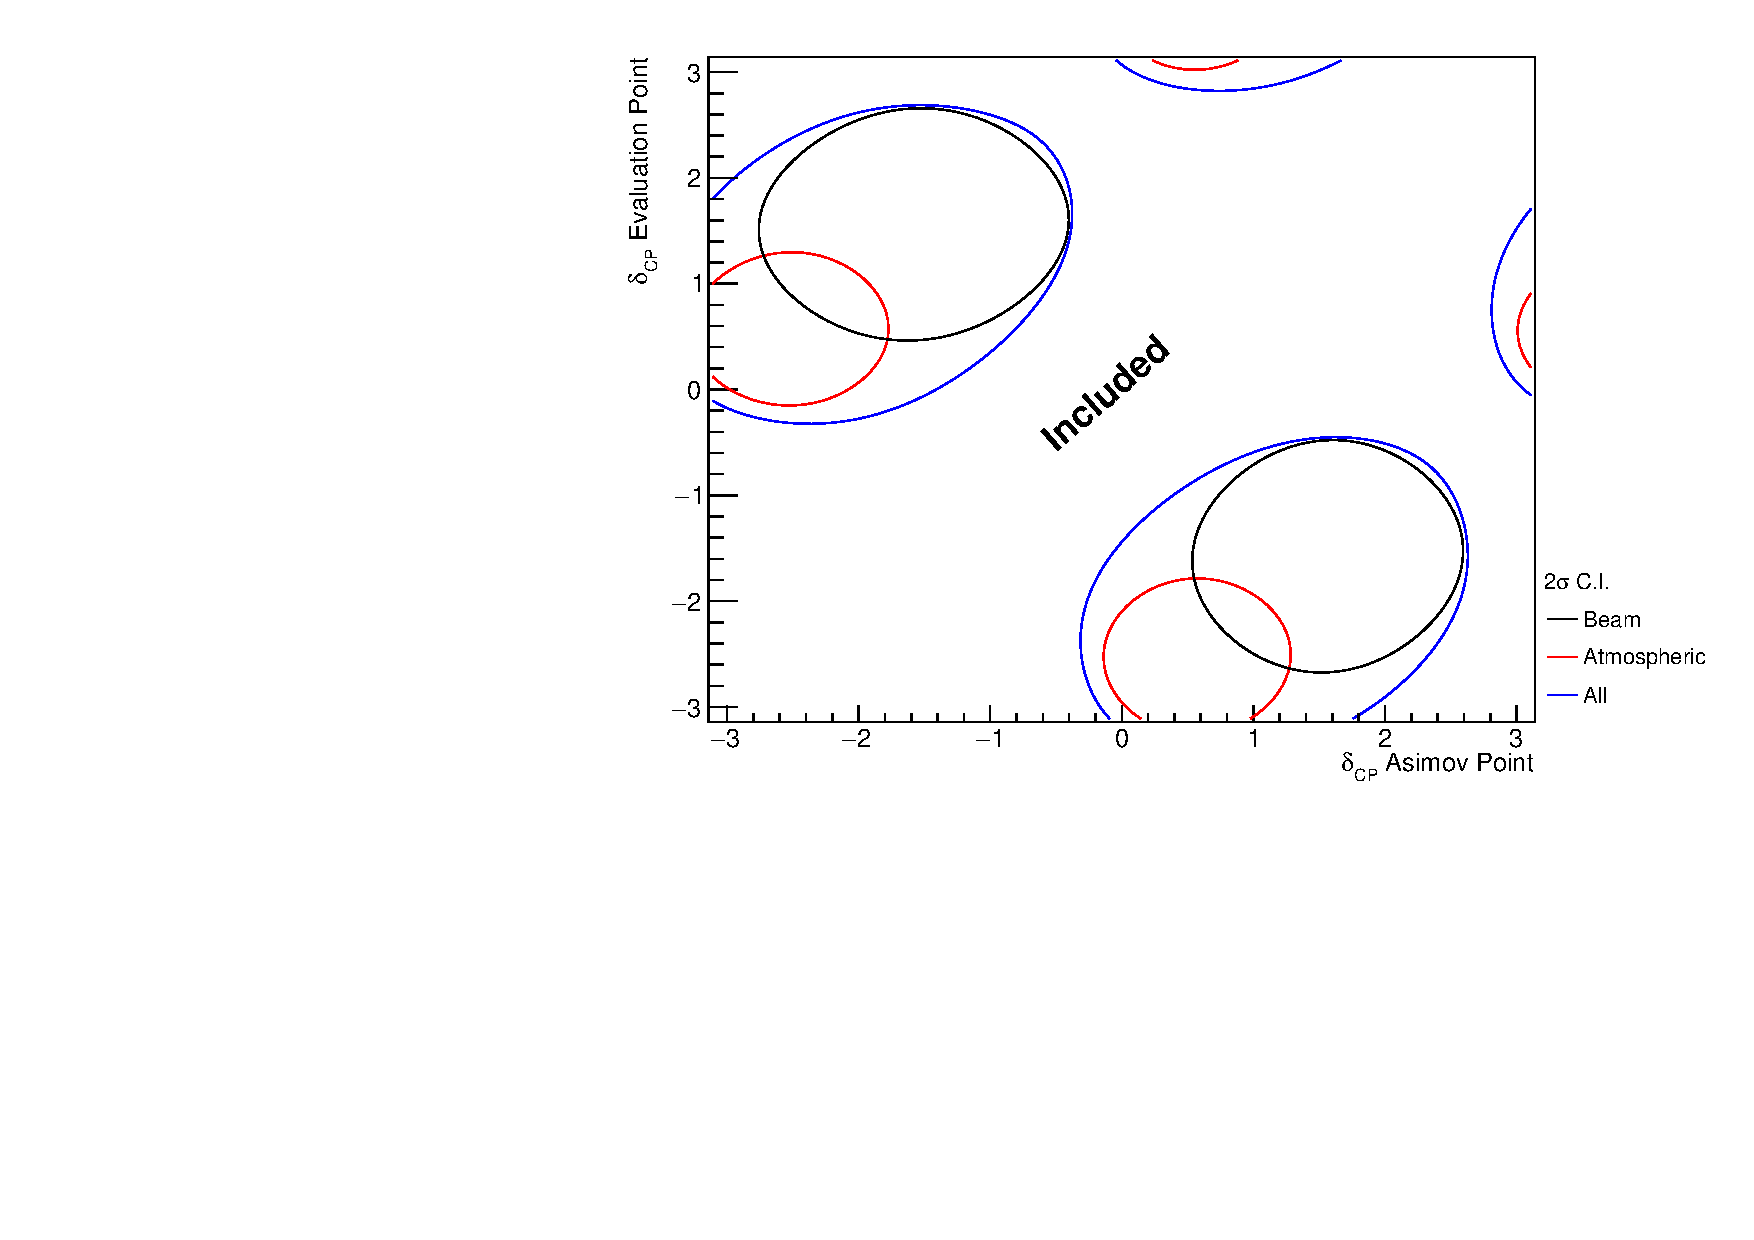
\includegraphics[width=\textwidth, trim={0mm 0mm 0mm 0mm}, clip,page=1]{Figures/OA/DCP_Scans_2Sig.pdf}
  \end{subfigure}
  \caption{A series of one-dimensional log-likelihood scans over \dcp, where an asimov data set is built for each value of \dcp on the x-axis and the log-likelihood is evaluated for each value on the y-axis. The diagonal represents the minimum log-likelihood and defines the region included within the \quickmath{1\sigma} (Top) and \quickmath{2\sigma} (Bottom) confidence intervals. The beam (black) and atmospheric (red) samples are individually plotted and the joint fit (blue) is the sum of the two.}
  \label{fig:OscillationAnalysis_AsimovEval_DCP}
\end{figure}

\begin{figure}[h]
  \begin{subfigure}[t]{1.0\textwidth}
    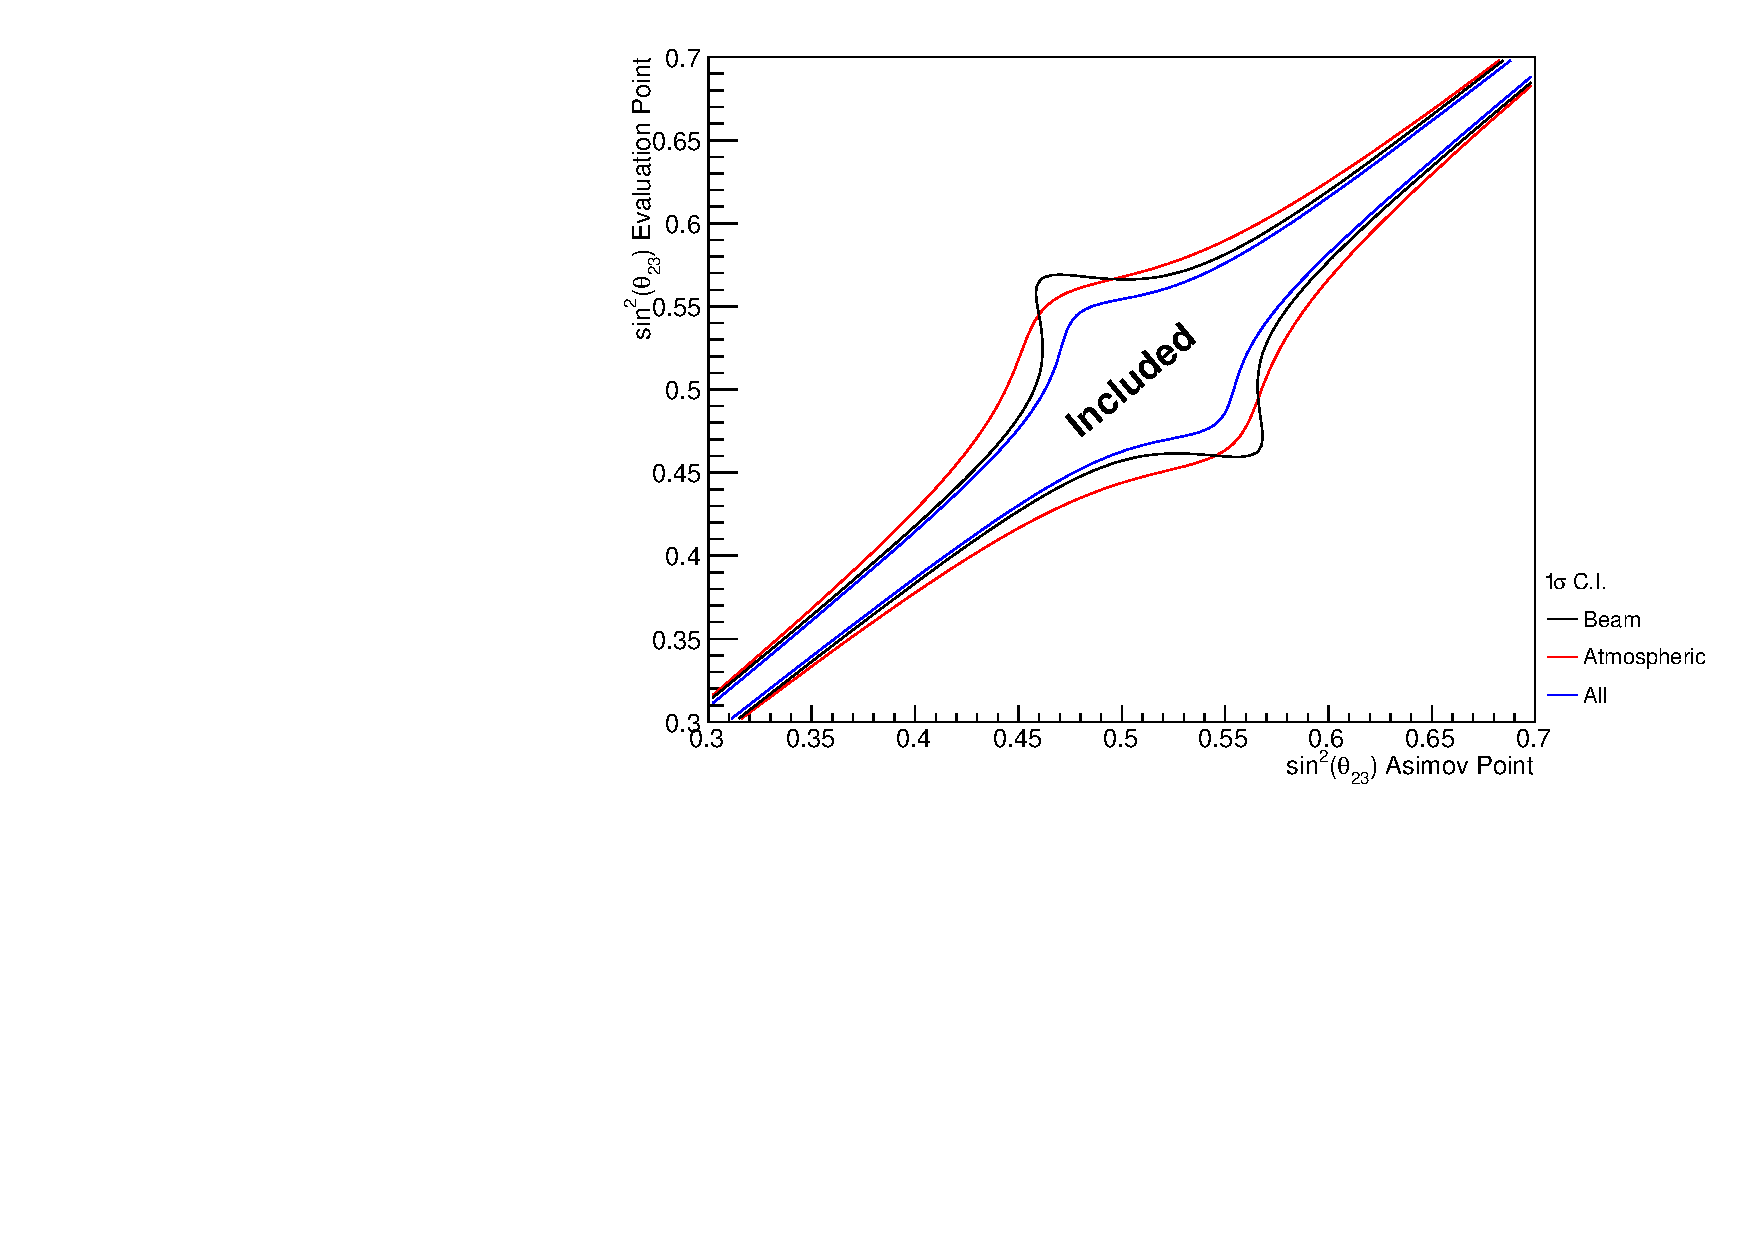
\includegraphics[width=\textwidth, trim={0mm 0mm 0mm 0mm}, clip,page=1]{Figures/OA/TH23_Scans_1Sig.pdf}
  \end{subfigure}                                                                                                                                                                                          
  \begin{subfigure}[t]{1.0\textwidth}
    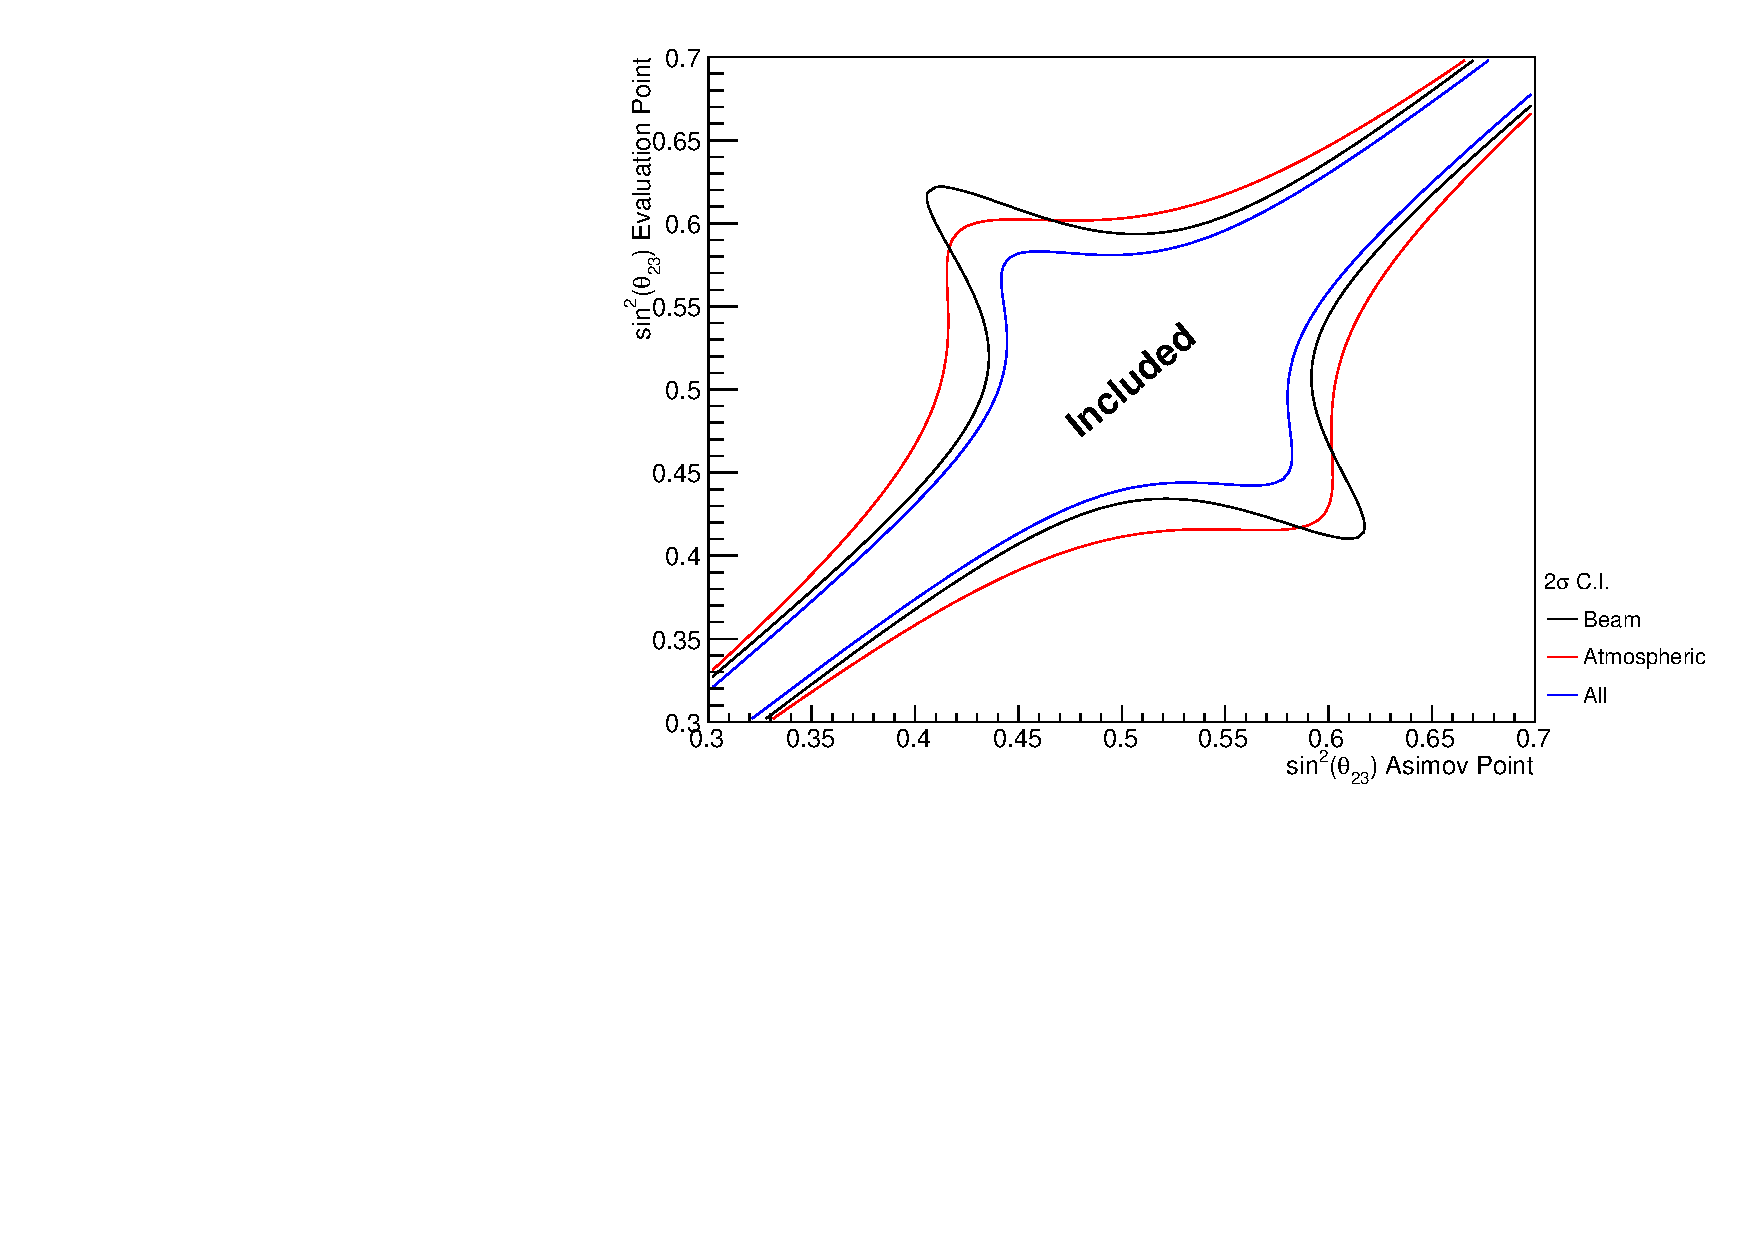
\includegraphics[width=\textwidth, trim={0mm 0mm 0mm 0mm}, clip,page=1]{Figures/OA/TH23_Scans_2Sig.pdf}
  \end{subfigure}
  \caption{A series of one-dimensional log-likelihood scans over \sinsqatm, where an asimov data set is built for each value of \sinsqatm on the x-axis and the log-likelihood is evaluated for each value on the y-axis. The diagonal represents the minimum log-likelihood and defines the region included within the \quickmath{1\sigma} (Top) and \quickmath{2\sigma} (Bottom) confidence intervals. The beam (black) and atmospheric (red) samples are individually plotted and the joint fit (blue) is the sum of the two.}
  \label{fig:OscillationAnalysis_AsimovEval_TH23}
\end{figure}

\clearpage

Alongside oscillation parameters, the sensitivity to systematic parameters can also be studied. As some of these parameters are correlated between the beam and atmospheric events, the addition of the atmospheric samples can modify the near detector constraint producing results which could have differing constraints than a T2K-only analysis. Consequently, the relative strength of the response between beam and atmospheric samples has been compared for various systematic parameters in \autoref{fig:OscillationAnalysis_LLHScanSystPars}. For example, the systematic parameter controlling the effective axial mass coupling in CCQE interactions, \texttt{MAQE}, is clearly dominated by the ND constraint. An example where the atmospheric samples response is approximately similar to the near detector constraint is the \texttt{2p2h\_CtoO} normalisation systematic. There are also systematics which have no near detector constraint, for example the systematic parameters which describe the normalisation of the NC1Gamma and NCOther interaction modes. The atmospheric samples are significantly more sensitive to these systematics than the beam samples. As an example of how the atmospheric samples can help constrain systematic parameters used within the T2K-only analysis, the neutral current background events in beam electron-like samples will be considerably more constrained with the additional sensitivity observed in \autoref{fig:OscillationAnalysis_LLHScanSystPars}. This would be expected to reduce the overall uncertainty on the beam electron-like event rates in the joint analysis compared to the beam-only studies.

\begin{figure}[h]
  \begin{subfigure}[t]{0.5\textwidth}
    \includegraphics[width=\textwidth, trim={0mm 0mm 0mm 0mm}, clip,page=2]{Figures/OA/LLHScans_Systs.pdf}
    \subcaption{\texttt{MAQE}}
  \end{subfigure}%
  \begin{subfigure}[t]{0.5\textwidth}
    \includegraphics[width=\textwidth, trim={0mm 0mm 0mm 0mm}, clip,page=5]{Figures/OA/LLHScans_Systs.pdf}
    \subcaption{\texttt{2p2h\_CtoO} Norm.}
  \end{subfigure}
  \begin{subfigure}[t]{0.5\textwidth}
    \includegraphics[width=\textwidth, trim={0mm 0mm 0mm 0mm}, clip,page=41]{Figures/OA/LLHScans_Systs.pdf}
    \subcaption{NC1Gamma Norm.}
  \end{subfigure}%
  \begin{subfigure}[t]{0.5\textwidth}
    \includegraphics[width=\textwidth, trim={0mm 0mm 0mm 0mm}, clip,page=43]{Figures/OA/LLHScans_Systs.pdf}
    \subcaption{NC Other Norm.}
  \end{subfigure}
  \begin{subfigure}[t]{0.5\textwidth}
    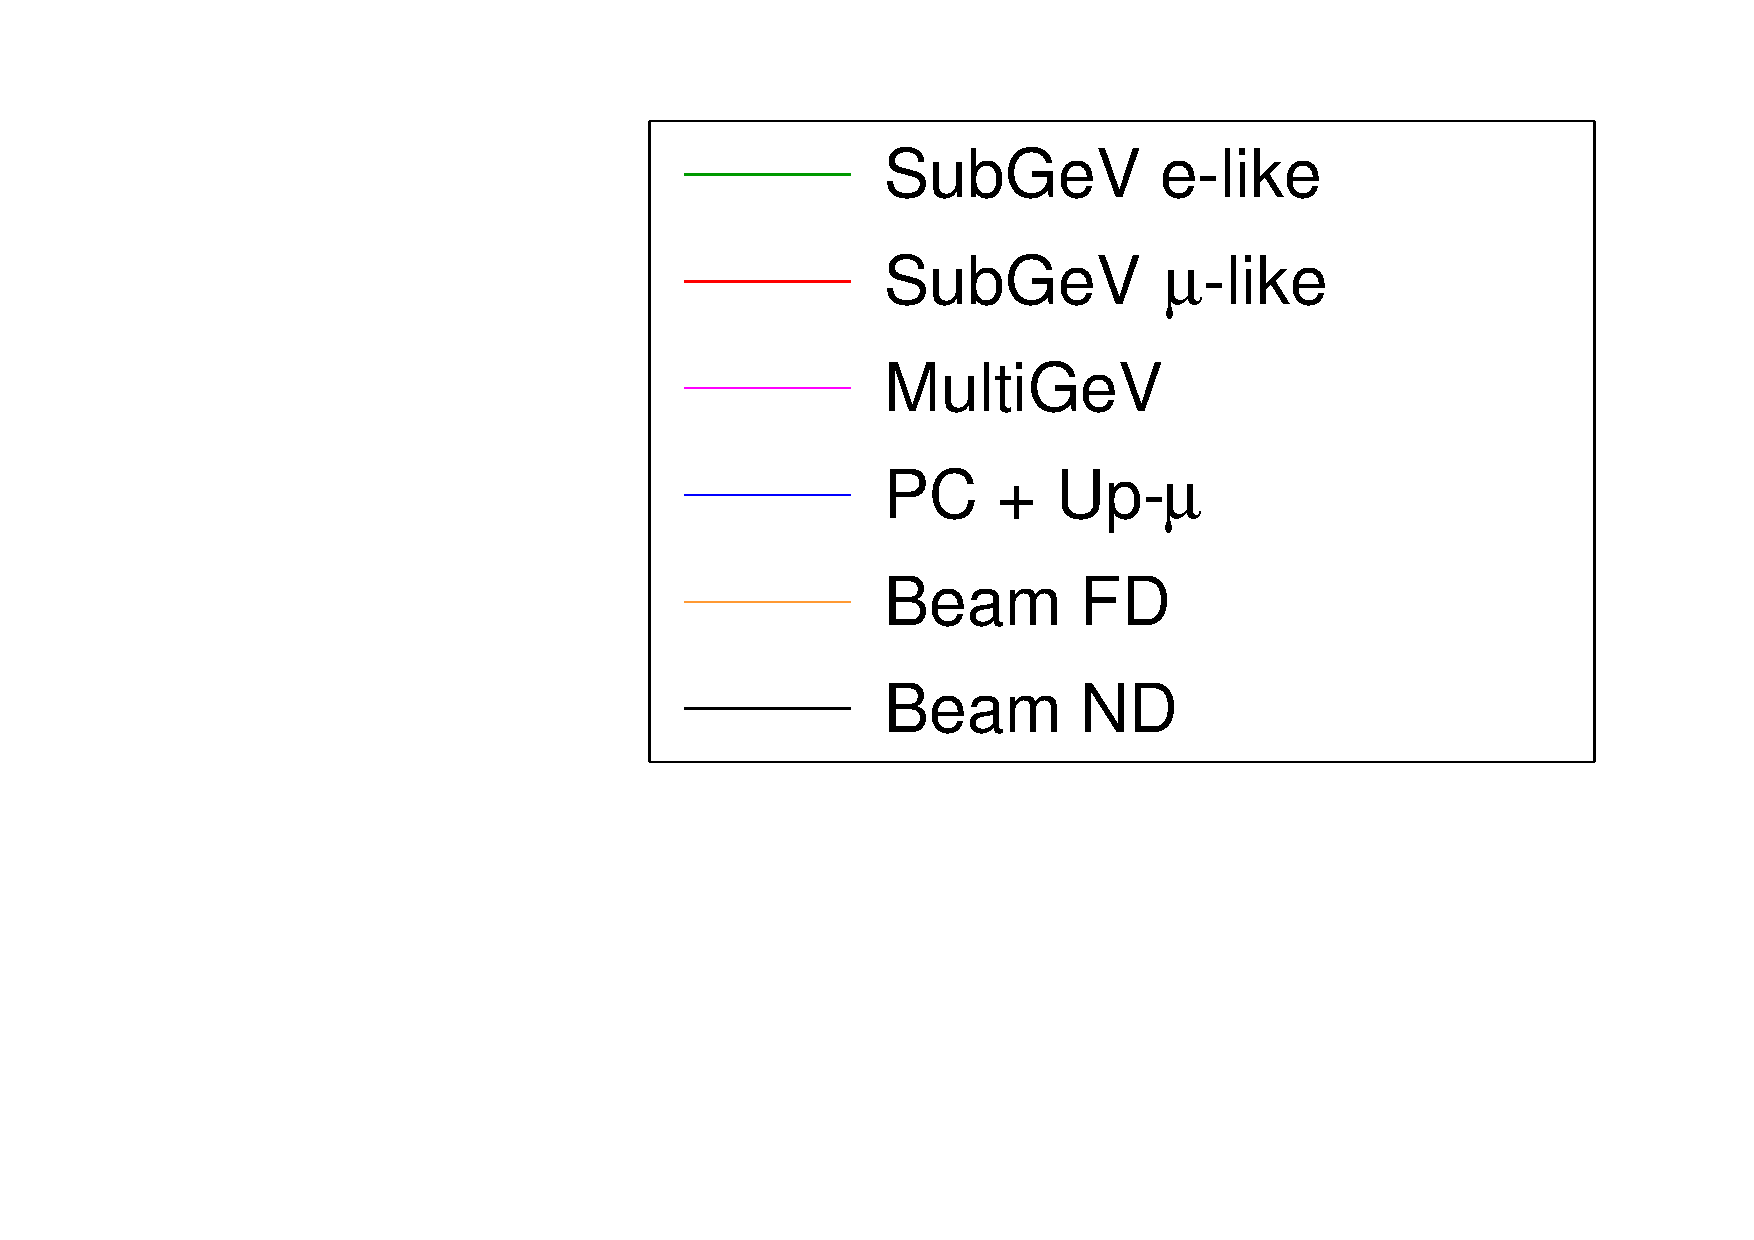
\includegraphics[width=\textwidth, trim={0mm 0mm 0mm 0mm}, clip,page=1]{Figures/OA/LLHScans_Systs.pdf}
  \end{subfigure}
  \caption{The response of the likelihood, as defined in section 8.2, illustrating the response of the samples to the various cross-section systematic parameters. The Asimov data set is built using the pre-fit dial values assuming Asimov A oscillation parameters defined in \autoref{tab:Theory_ParameterSets}.}
  \label{fig:OscillationAnalysis_LLHScanSystPars}
\end{figure}

\clearpage
\section{Sensitivities}
\label{sec:OscillationAnalysis_Sensitivities}

The sensitivities of the joint T2K and SK oscillation analysis are presented in the form of Asimov fits. This technique builds a fake `data' prediction of each sample's spectra from the Monte Carlo, reweighted to a particular set of oscillation and systematic parameters. This prediction is then used as data in which to fit against. Whilst this results in unphysical non-integer data predictions, it eliminates statistical fluctuations from the data. Therefore, the results of a fit to Asimov data should not include any biases from statistical fluctuations. Furthermore, these results should produced posterior probability distributions conistent with the parameters which were used to make the data prediction. That is to say, the fit results should return the known parameters. Any biases seen would be attributed to the a correlations between each oscillation parameter and correlations between oscillation and systematic parameters. Consequently, Asimov fit results present the maximum precision at which the oscillation parameters could be measured to.

In practice, the asimov fits presented within this analysis are modified from the above definition. An asimov prediction of both beam and atmospheric far detector samples is fit whilst the true data is used for near detector samples. The asimov predictions at the far detector are built using the BANFF tuning (as discussed in \autoref{sec:T2KSKExp_T2K}). This is equivalent to performing a far detector asimov fit using inputs from the BANFF data fit. Consequently, this allows the results to be cross-checked to the P-Theta analysis.

\subsection{Atmospheric-Only Sensitivity Without Reactor Constraint}
\label{sec:OscillationAnalysis_SKOnly}

This section presents the results of an asimov fit using samples from the near detector and only atmospheric samples from the far detector. The results are marginalised over the nuisance parameters using the technique outlined in \autoref{sec:MarkovChainMonteCarlo_Marginalisation}. Each histogram displays the posterior probability density at each point within the parameter space. One dimensional histograms illustrate the \quickmath{1}, \quickmath{2} and \quickmath{3\sigma} credible intervals, calculated using the technique discussed in \autoref{sec:MarkovChainMonteCarlo_ParameterEstimation}. For these fits, a flat penalty term is used for \sinsqreac (i.e. the reactor constraint is not applied). The asimov data is generated assuming the AsimovA oscillation parameter set defined in \autoref{tab:Theory_ParameterSets} and the post-BANFF systematic parameter tune.

The posterior probability density in \delmsqatm is given in \autoref{fig:OscillationAnalysis_SKOnly_DM32}. This distribution includes steps in both the normal hierarchy \quickmath{\left(\text{NH, } \Delta m^{2}_{32} > 0 \right)} and the inverse hierarchy \quickmath{\left(\text{IH, } \Delta m^{2}_{32} < 0 \right)}. The highest posterior density is found within the NH, which agrees with the asimov point. However, all of the credible intervals span both hierarchies. This is the result of marginalising over both hierarchies. If instead, only steps in the normal hierarchy were considered, the shape of the contours would change. The known oscillation parameter is \quickmath{2.509 \times 10^{-3} \text{eV}^{2}}, which is contained within the \quickmath{1\sigma} credible interval.

\begin{figure}[h]
  \begin{subfigure}[t]{1.0\textwidth}
    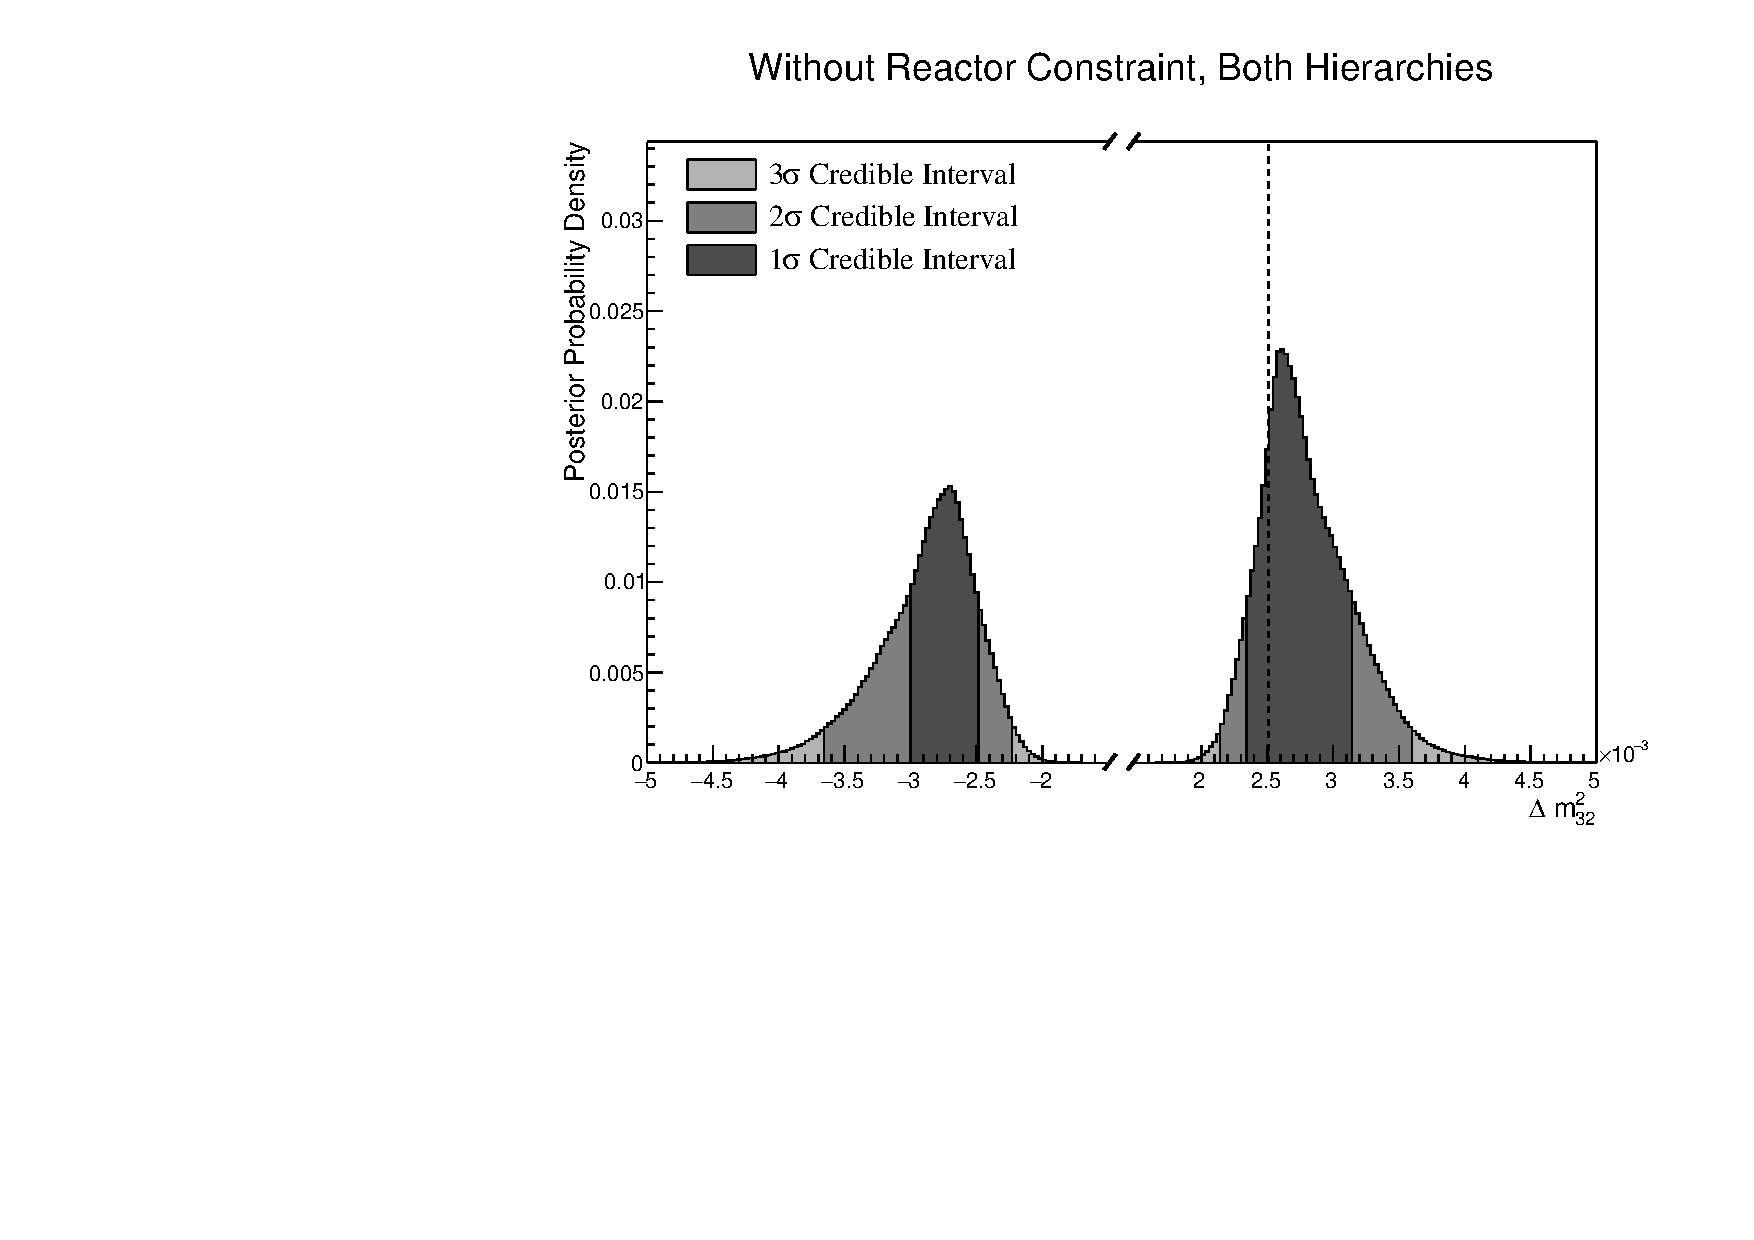
\includegraphics[width=\textwidth, trim={0mm 0mm 0mm 0mm}, clip,page=1]{Figures/OA/SKOnlyFit/Contours_1D_dm32_BH_1_woRC_UnSmeared_CredibleInterval.pdf}
  \end{subfigure}
  \caption{}
  \label{fig:OscillationAnalysis_SKOnly_DM32}
\end{figure}

Following the discussion in \autoref{sec:MarkovChainMonteCarlo_BayesTheorem}, the Bayes factor for hierarchy preference can be calculated by determining the fraction of steps which fall into the NH and the IH, as an equal prior is placed on both models. A similar analysis can be performed by calculating the fraction of steps which fall in the lower octant \quickmath{\left(\text{LO, } \sin^{2}\theta_{23} < 0.5 \right)} or upper octant \quickmath{\left(\text{UO, } \sin^{2}\theta_{23} > 0.5 \right)}. The fraction of steps, broken down by hierarchy and octant, are given in \autoref{tab:OscillationAnalysis_SKOnly_BayesFactors}. The Bayes factor for preffered hierarchy model is \quickmath{B(\text{NH}/\text{IH}) = 1.37}. \autoref{tab:MarkovChainMonteCarlo_JeffreysScale} states this value of the Bayes factor indicates a weak preference for the normal hierarchy model. The Bayes factor for choice of octant is \quickmath{B(\text{UO}/\text{LO}) = 2.24}. This is also classified as a weak preference for the UO. Both of these show that the fit is returning the correct choice of models (NH and UO) for the known Asimov A oscillation parameters defined in \autoref{tab:Theory_ParameterSets}. 

\begin{table}[ht!]
  \centering
  \begingroup
  \renewcommand{\arraystretch}{1.5}
  \begin{tabular}{c|cc|c}
                                                        & LO \quickmath{\left(\sin^{2}\theta_{23} < 0.5 \right)} & UO \quickmath{\left( \sin^{2}\theta_{23} > 0.5 \right)} & Sum  \\ \hline
    NH \quickmath{\left( \Delta m^{2}_{32} > 0 \right)} &                                                   0.17 &                                                    0.40 & 0.58 \\
    IH \quickmath{\left( \Delta m^{2}_{32} < 0 \right)} &                                                   0.13 &                                                    0.29 & 0.42 \\ \hline
    Sum                                                 &                                                   0.31 &                                                    0.69 & 1.00 \\       
  \end{tabular}
  \caption{}
  \label{tab:OscillationAnalysis_SKOnly_BayesFactors}
  \endgroup
\end{table}

\begin{figure}[h]
  \begin{subfigure}[t]{1.0\textwidth}
    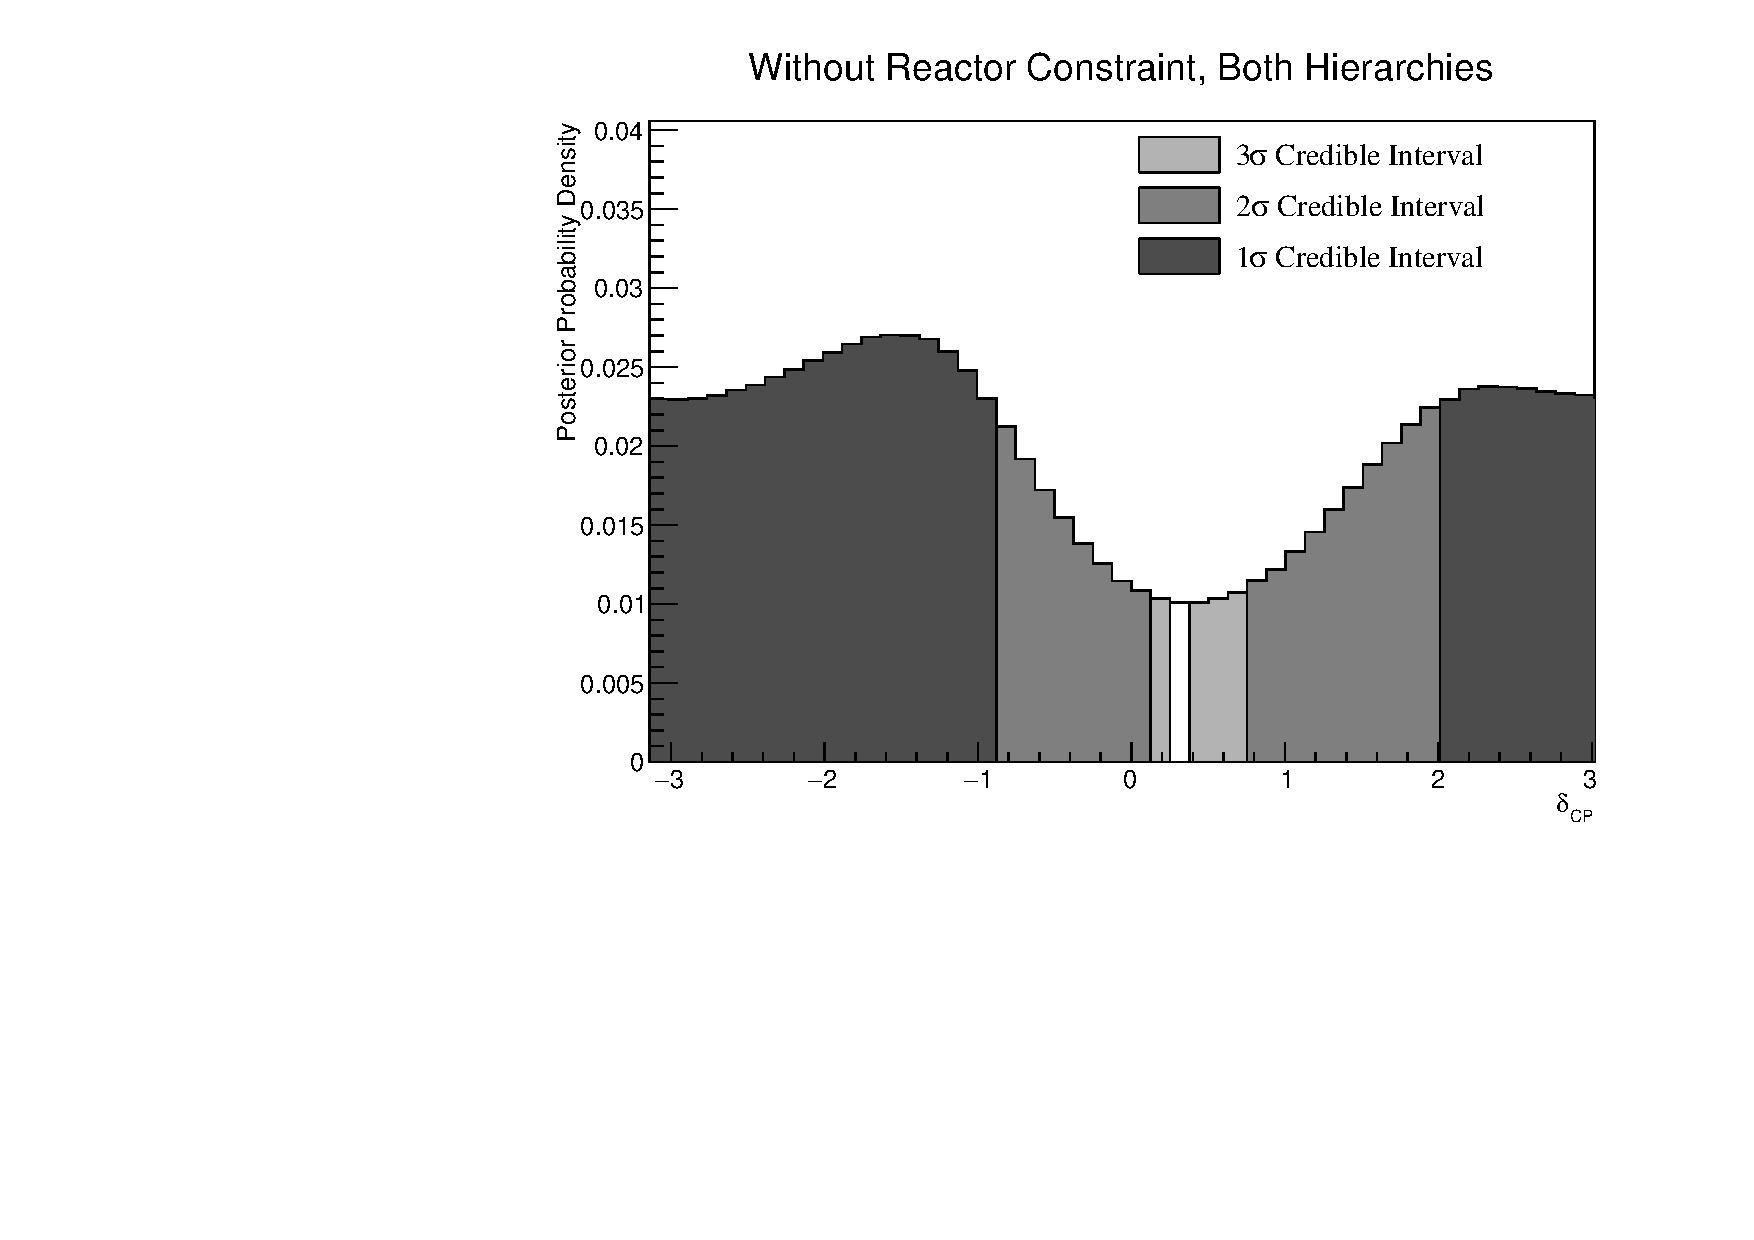
\includegraphics[width=\textwidth, trim={0mm 0mm 0mm 0mm}, clip,page=1]{Figures/OA/SKOnlyFit/Contours_1D_dcp_BH_1_woRC_UnSmeared_CredibleInterval.pdf}
  \end{subfigure}
  \caption{}
  \label{fig:OscillationAnalysis_SKOnly_DCP}
\end{figure}

\autoref{fig:OscillationAnalysis_SKOnly_DCP} illustrates the posterior probability density for \quickmath{\delta_{CP}}, marginalised over both hierarchies. The fit does favour the asimov position (\quickmath{\delta_{CP} = -1.601}) although the posterior probability is very flat through the of \quickmath{2 < \delta_{CP} < \pi} and \quickmath{-\pi < \delta_{CP} < -1}. There is also a region around \quickmath{\delta_{CP} \sim 0.4} which is disfavoured at \quickmath{2\sigma}. This indicates that the SK samples can rule out some parts of the CP conserving parameter space reasonably well, near \quickmath{\delta_{CP} \sim 0}, when the true value of \quickmath{\delta_{CP}} is CP violating. 

\begin{table}[ht!]
  \centering
  \begingroup
  \renewcommand{\arraystretch}{1.5}
  \begin{tabular}{c|c|c}
    Parameter               & Interval & HPD \\ \hline
    \quickmath{\delta_{CP}, \text{ (BH)}} & \quickmath{\left[ -\pi, -0.86 \right], \left[ 1.96, \pi \right]} & -1.57 \\
    \quickmath{\delta_{CP}, \text{ (NH)}} & \quickmath{\left[ -\pi, -0.86 \right], \left[ 1.88, \pi \right]} & -1.57 \\
    \quickmath{\delta_{CP}, \text{ (IH)}} & \quickmath{\left[ -\pi, -0.94 \right], \left[ 1.96, \pi \right]} & -1.57 \\ \hline
    \quickmath{\Delta m^{2}_{32} \text{ (BH) } [\times 10^{-3} \text{eV}^{2}]} & \quickmath{\left[ -3.00, -2.50 \right], \left[ 2.35, 3.15 \right]} & 2.65 \\
    \quickmath{\Delta m^{2}_{32} \text{ (NH) } [\times 10^{-3} \text{eV}^{2}]}& \quickmath{\left[ 2.39, 3.04 \right]} & 2.64 \\
    \quickmath{\Delta m^{2}_{32} \text{ (IH) } [\times 10^{-3} \text{eV}^{2}]} & \quickmath{\left[ -3.15, -2.45 \right]} & -2.70 \\ \hline
    \quickmath{\sin^{2}(\theta_{23}) \text{ (BH) }} & \quickmath{\left[ 0.476, 0.59 \right]} & 0.542 \\ 
    \quickmath{\sin^{2}(\theta_{23}) \text{ (NH) }} & \quickmath{\left[ 0.476, 0.59 \right]} & 0.554 \\ 
    \quickmath{\sin^{2}(\theta_{23}) \text{ (IH) }} & \quickmath{\left[ 0.476, 0.59 \right]} & 0.542 \\ \hline \hline
  \end{tabular}
  \caption{}
  \label{tab:OscillationAnalysis_SKOnly_CredIntervals}
  \endgroup
\end{table}

The \quickmath{1\sigma} credible intervals, broken down by hierarchy, and position in parameter space of the highest posterior density is given in \autoref{tab:OscillationAnalysis_SKOnly_CredIntervals}. These are taken from the one dimensional projections of the oscillation parameters, marginalised over all other parameters within the fit. For the known asimov value of \quickmath{\delta_{CP} = -1.601}, the \quickmath{1\sigma} credible interval rules out a regiion between \quickmath{\delta_{CP} = -0.86} and \quickmath{\delta_{CP} = 1.96}, when marginalising over both hierarchies. Interestingly, when considering the width of the interval when only considering steps in the NH, the intervals become narrower and the results excludes a large region of phase space. Thus, if the hierarchy model is known before the fit, the constraint would be stronger. The \quickmath{1\sigma} credible intervals for \quickmath{\sin^{2}(\theta_{23})} were found to be the same in all three hierarchy choices (marginalised over both, NH and IH). This illustrates that the distribution of \quickmath{\sin^{2}(\theta_{23})} is symmetric across the hierarchy discontinuity.

As expected, the width of the credible intervals in \delmsqatm is smaller when only the NH is considered compared to when both models are marginalised over. This follows from the fit weakly preferring the NH model over the IH model. Conversely, when the credible intervals are built using only IH steps, the credible intervals are wider than when both hierarchies are considered.

The sensitivity of the atmospheric samples to \sinsqreac is presented in \autoref{fig:OscillationAnalysis_SKOnly_TH13}. The likelihood scans presented in \autoref{fig:OscillationAnalysis_LLHScanOscPars} suggest that the sensitivity to \sinsqreac will be small. This is seen from the fit results, where the width of the \quickmath{1\sigma} credible intervals span the region of \quickmath{\sin^{2}(\theta_{13}) = [0.008, 0.08]}. This is an order of magnitude larger than the reactor constraint.

\begin{figure}[h]
  \begin{subfigure}[t]{1.0\textwidth}
    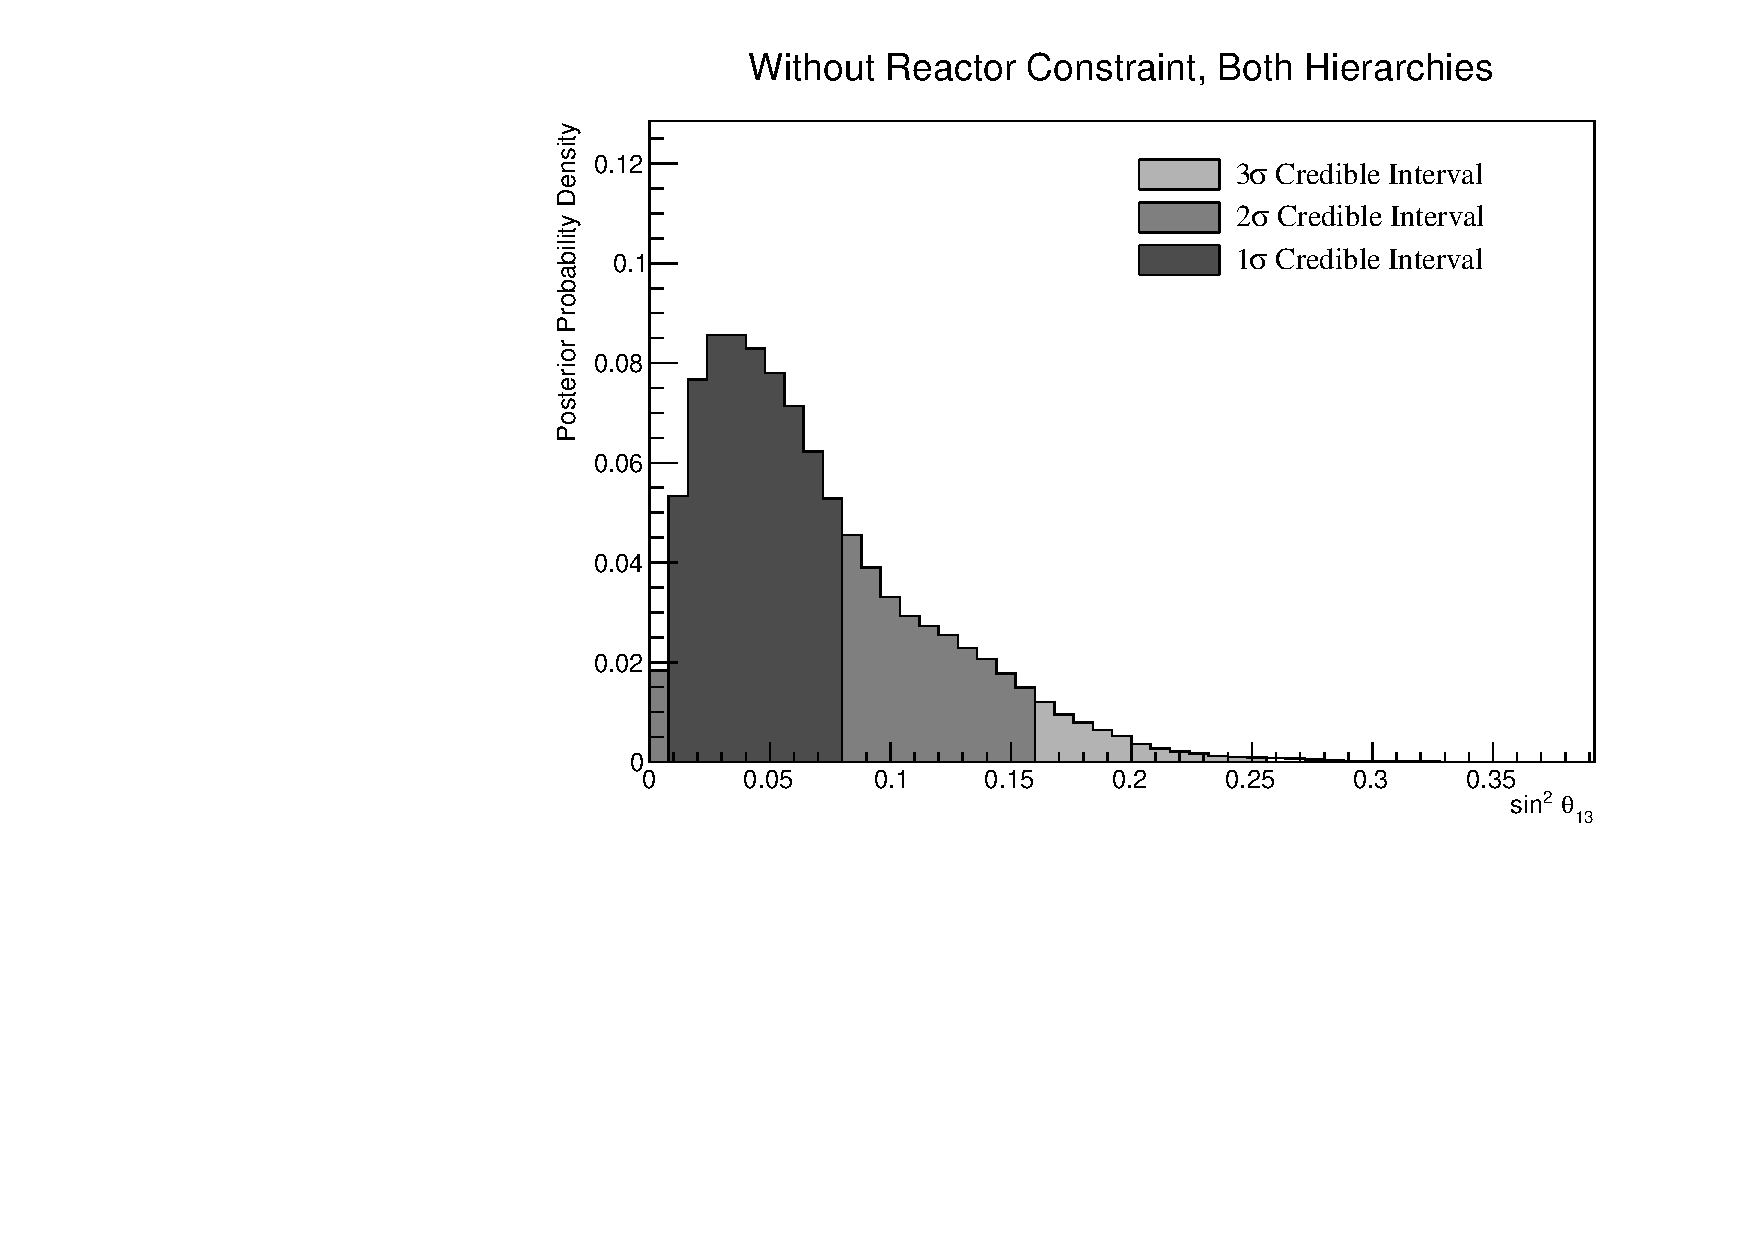
\includegraphics[width=\textwidth, trim={0mm 0mm 0mm 0mm}, clip,page=1]{Figures/OA/SKOnlyFit/Contours_1D_th13_BH_1_woRC_UnSmeared_CredibleInterval.pdf}
  \end{subfigure}
  \caption{}
  \label{fig:OscillationAnalysis_SKOnly_TH13}
\end{figure}

\begin{figure}[h]
  \begin{subfigure}[t]{1.0\textwidth}
    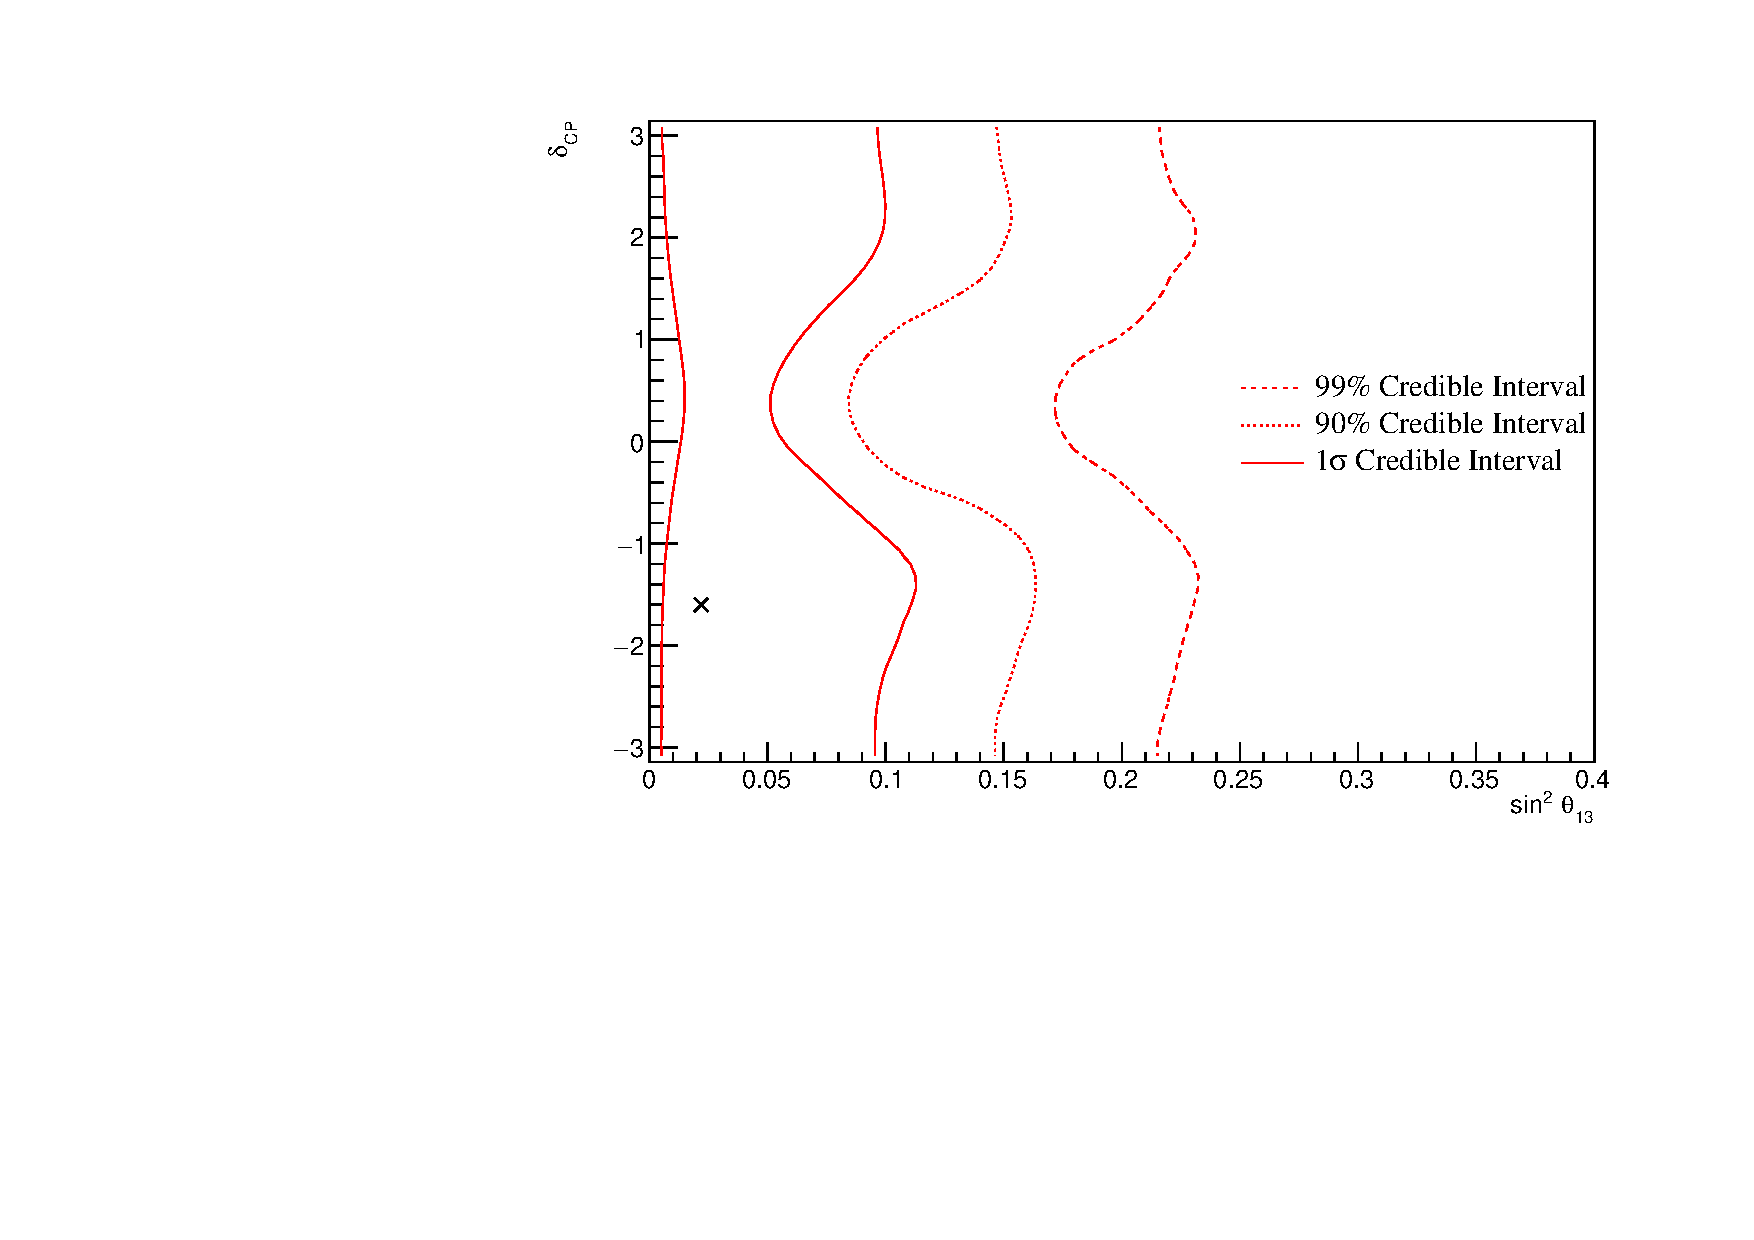
\includegraphics[width=\textwidth, trim={0mm 0mm 0mm 0mm}, clip,page=1]{Figures/OA/SKOnlyFit/Contours_2D_th13_dcp_BH_0_woRC_UnSmeared_CredibleInterval.pdf}
  \end{subfigure}
  \caption{}
  \label{fig:OscillationAnalysis_SKOnly_DCPTH13}
\end{figure}

As prevously discussed, the correlations between oscillation parameters are also important to understand how the atmospheric samples respond. \autoref{fig:OscillationAnalysis_SKOnly_DCPTH13} illustrates the two dimensional \quickmath{\sin^{2}(\theta_{13}) - \delta_{CP}} projection of the full posterior probability distribution, marginalised over both hierarchies. The shape of the \quickmath{1\sigma} credible interval shows that the constraining power of the fit on \dcp is dependent upon the choice of \quickmath{\sin^{2}(\theta_{13})}. As expected from \autoref{fig:OscillationAnalysis_LLHScanOscPars}, the atmospheric samples do not strongly constrain the value of \quickmath{\sin^{2}(\theta_{13})}. However, the choice of preffered value of \quickmath{\sin^{2}(\theta_{13})} does impact the atmospherics sensitivity to \dcp. The \quickmath{1\sigma} credible interval is consistent with the reactor constraint.

The \quickmath{\sin^{2}(\theta_{23}) - \Delta m^{2}_{32}} disappearance contours are illustrated in \autoref{fig:OscillationAnalysis_SKOnly_DM32TH23}. As expected, the distribution in the inverted hierarchy is slightly smaller than that in the normal hierarchy. This follows from the Bayes factor showing weak preference for NH meaning that more of the steps will exist in the \quickmath{\Delta m^{2}_{32} > 0} region. The asimov points of \quickmath{\sin^{2}(\theta_{23}) = 0.528} and \quickmath{\Delta m^{2}_{32} = 2.509\times 10^{-3}\text{eV}^{2}} are clearly contained within the \quickmath{1\sigma} credible interval.

\begin{figure}[h]
  \begin{subfigure}[t]{1.0\textwidth}
    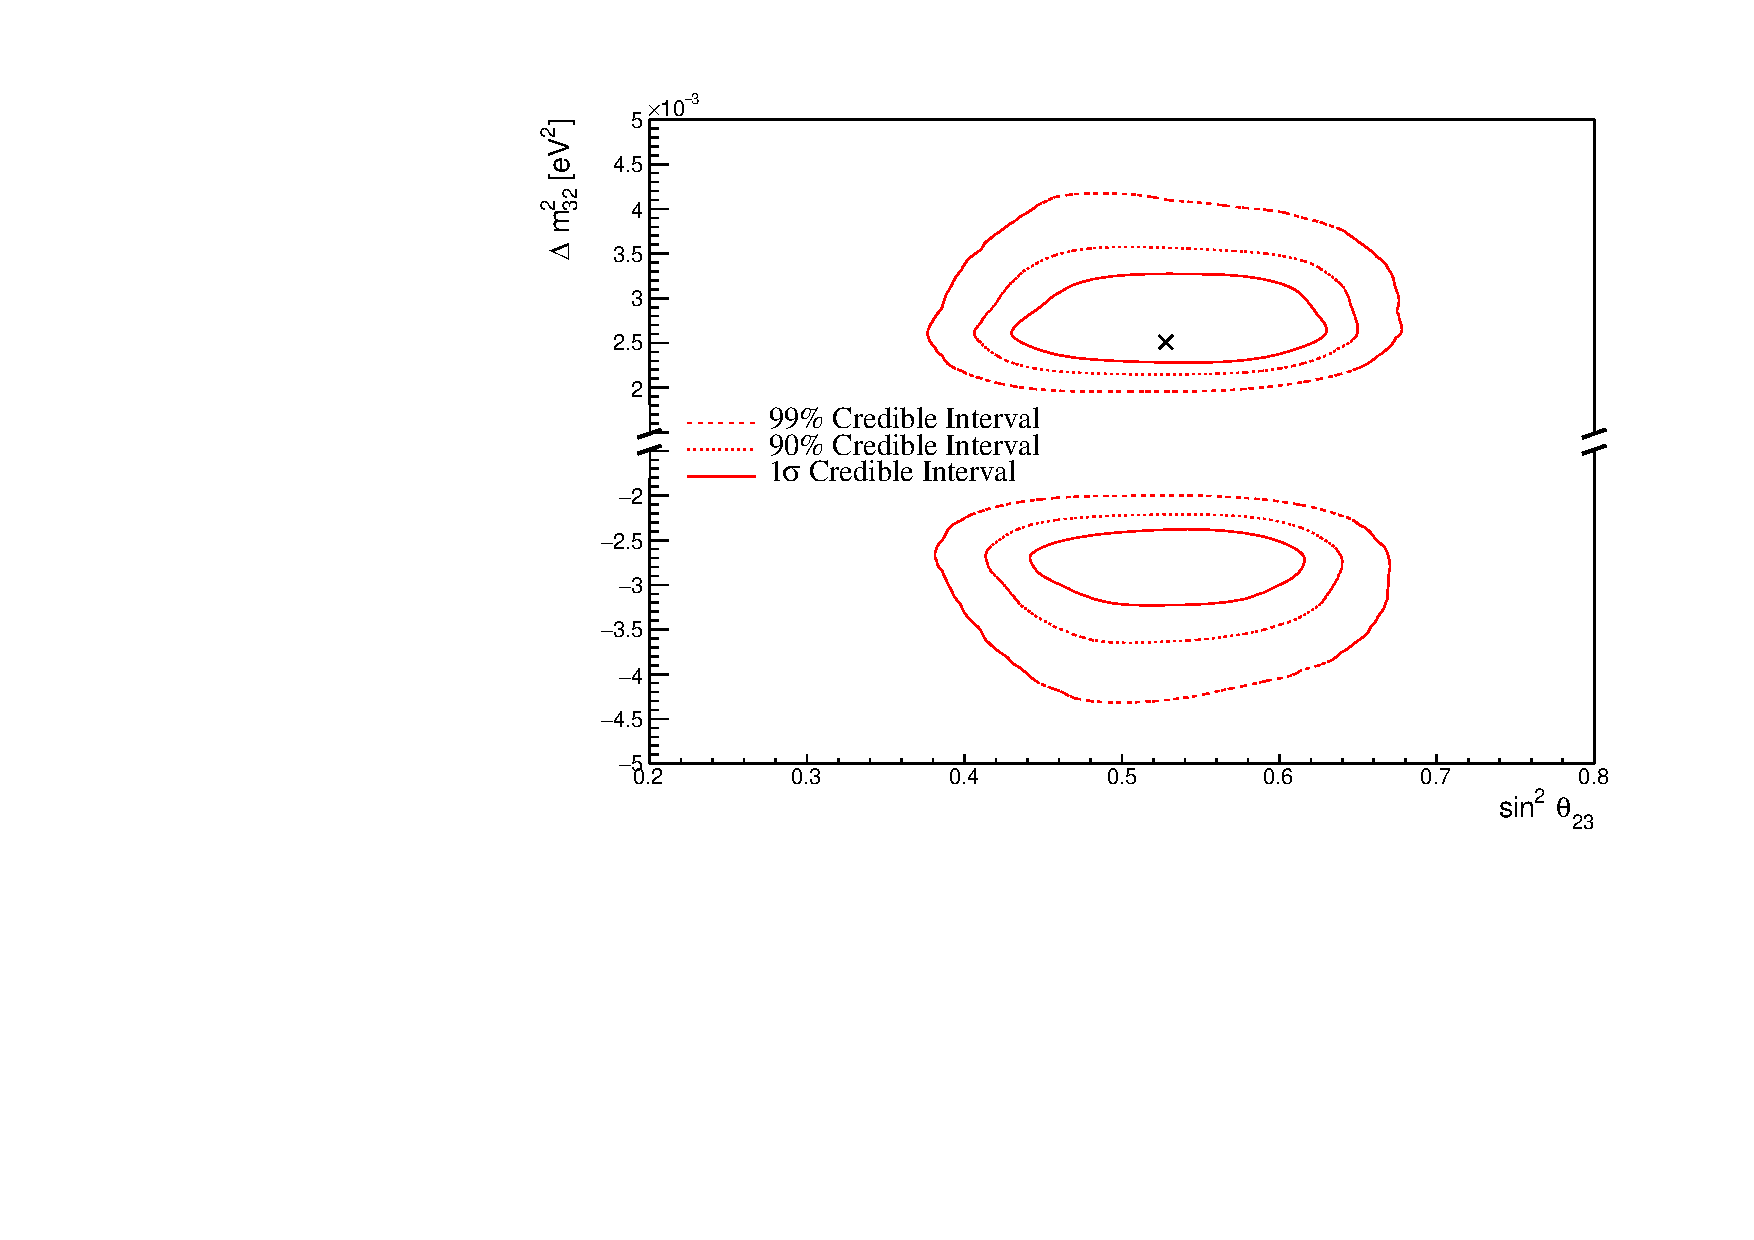
\includegraphics[width=\textwidth, trim={0mm 0mm 0mm 0mm}, clip,page=1]{Figures/OA/SKOnlyFit/Contours_2D_th23_dm32_BH_0_woRC_UnSmeared_CredibleInterval.pdf}
  \end{subfigure}
  \caption{}
  \label{fig:OscillationAnalysis_SKOnly_DM32TH23}
\end{figure}

\autoref{fig:OscillationAnalysis_SKOnly_TrianglePlot} highlights the two dimensional projections for each combination of oscillation parameters which this analysis is sensitive too. The contours are built when marginalising over both hierarchies but only the NH is illustrated when considering \delmsqatm. As expected the correlations play a significant role in these sensitivity measurements, especially the the choice of \sinsqreac constraint. The application of reactor constraint would be expected to alter both the width and position of the \delmsqatm credible interval and the width of the \dcp and \sinsqatm constraints. The majority of the octant model preference comes from the region of \quickmath{\sin^{2}(\theta_{13}) \sim 0.03}. Consequently, the application of the reactor constraint would not be expected to significantly change the octant preference. Interestingly, the distribution of steps in the \dcp-\sinsqreac plot is slightly flatter in the region of the reactor constraint. This follow from \autoref{fig:OscillationAnalysis_2DLLHOscScans_App} where the likelihood scan shows a region of low negative log-likelihood extending out towards higher values of \sinsqreac in the \quickmath{\delta_{CP} = -1.601} region. Consequently, the reactor constraint could feasibly reduce the sensitivity of the atmospheric samples to \dcp, due to these marginalisation effects. 

\begin{figure}[h]
  \begin{subfigure}[t]{1.0\textwidth}
    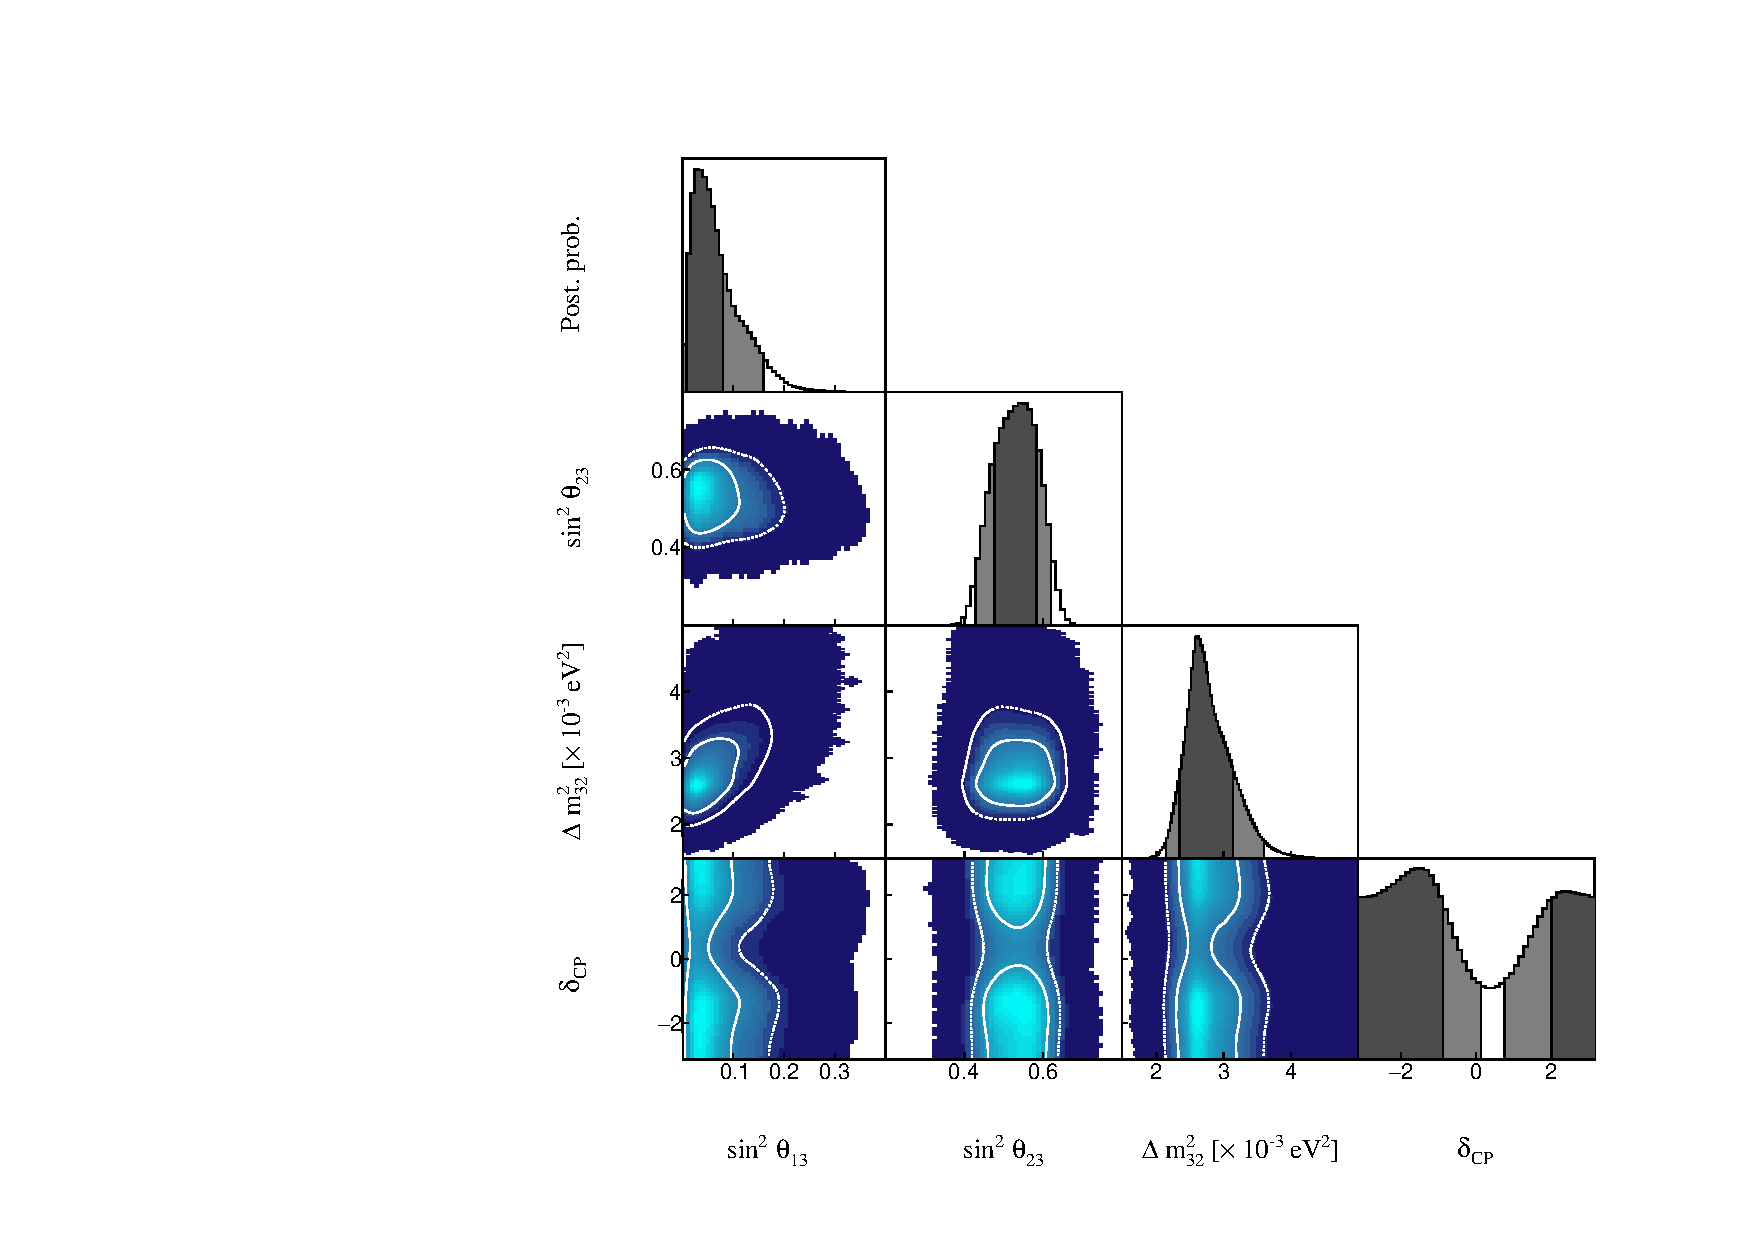
\includegraphics[width=\textwidth, trim={0mm 0mm 0mm 0mm}, clip,page=1]{Figures/OA/SKOnlyFit/Contours_1D_woRC_UnSmeared_CredibleInterval_TrianglePlot.pdf}
  \end{subfigure}
  \caption{}
  \label{fig:OscillationAnalysis_SKOnly_TrianglePlot}
\end{figure}

\clearpage
\subsection{Atmospheric-Only Sensitivity With Reactor Constraint}
\label{sec:OscillationAnalysis_SKOnly_wRC}

The results in \autoref{sec:OscillationAnalysis_SKOnly} discuss the atmospheric sensitivity when the reactor constraint is not applied. However, the correlations illustrated in \autoref{fig:OscillationAnalysis_SKOnly_TrianglePlot} indicate that the marginalisation effects could contribute to differing sensitivities when the external constraint is applied. Using the technique discussed in \autoref{sec:MarkovChainMonteCarlo_Priors}, the posterior distribution can be reweighted to include the reactor constraint of \quickmath{\sin^{2}(\theta_{13}) = \left(2.18 \pm 0.08\right) \times 10^{-2}}.

\begin{figure}[h]
  \begin{subfigure}[t]{1.0\textwidth}
    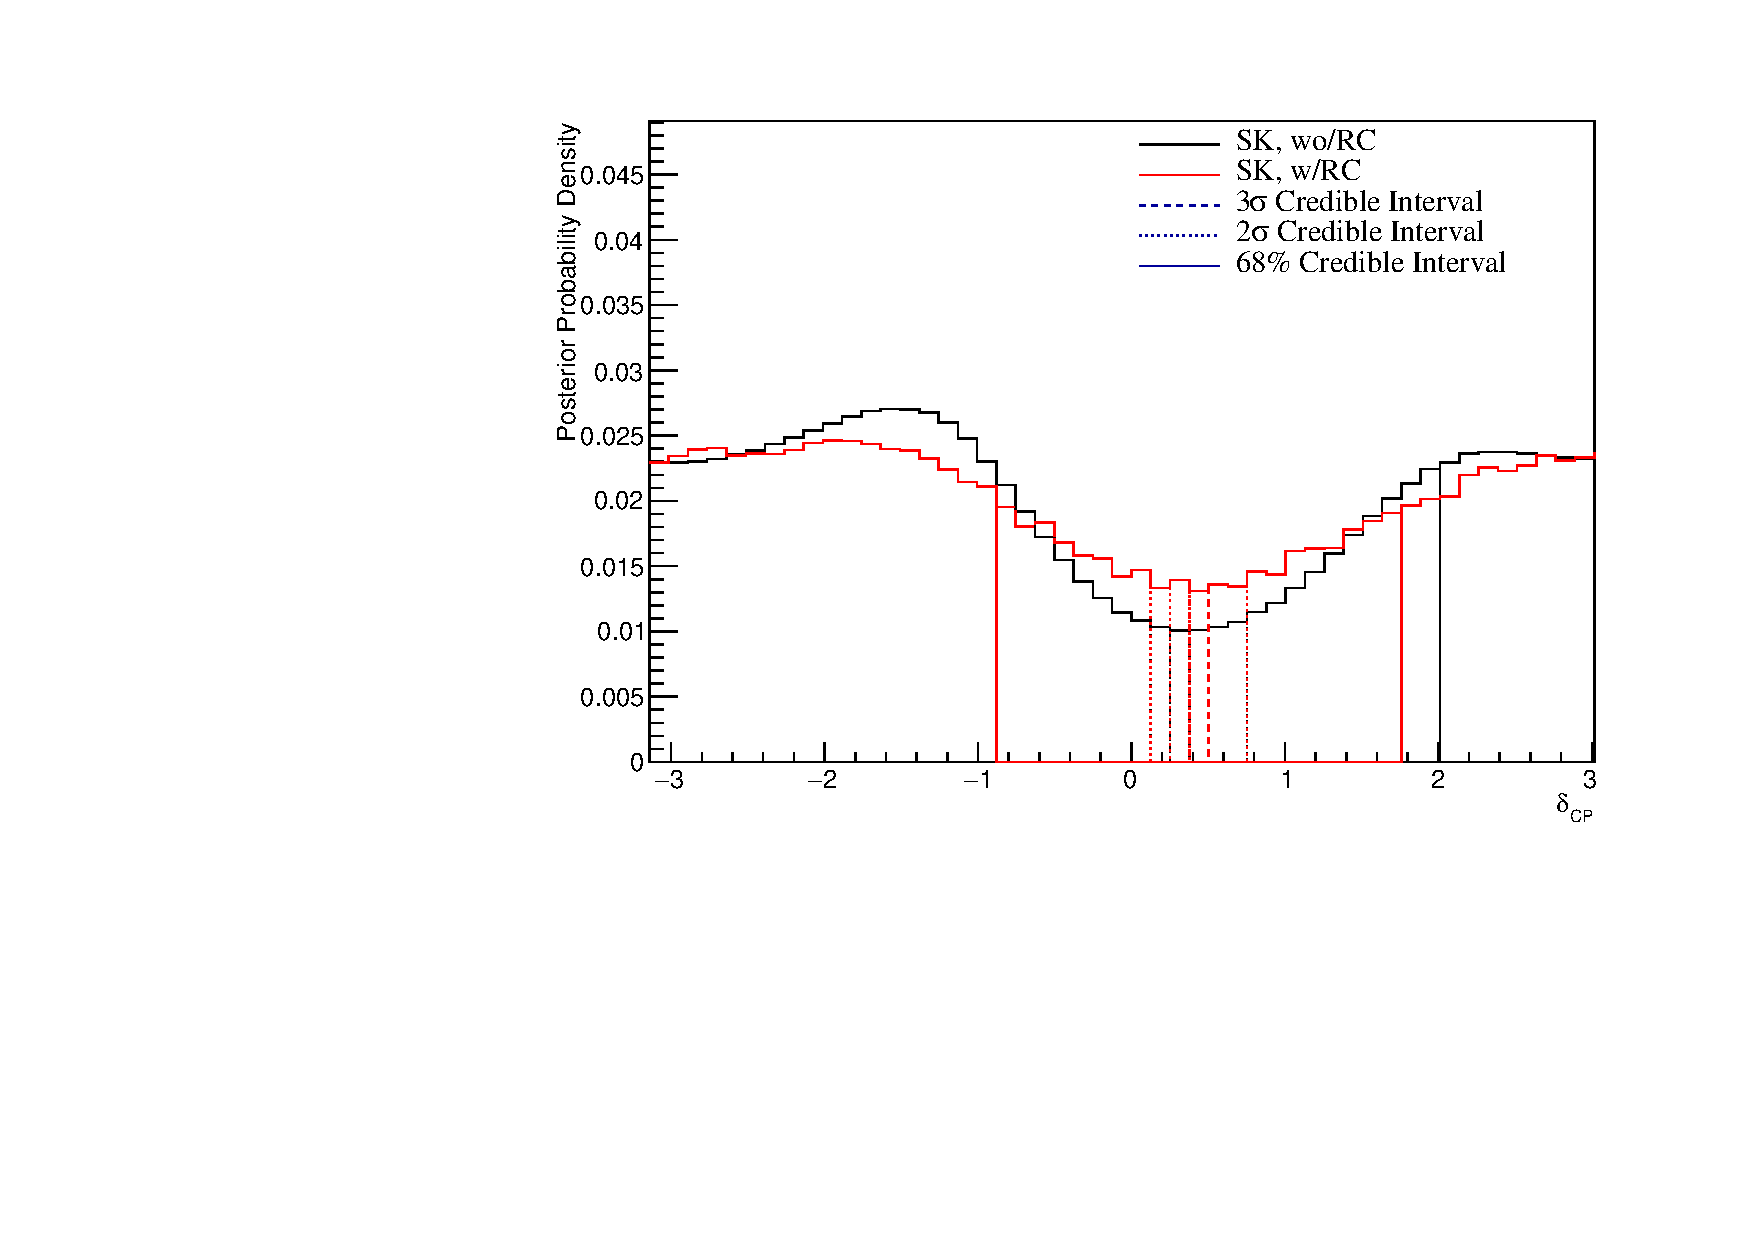
\includegraphics[width=\textwidth, trim={0mm 0mm 0mm 0mm}, clip,page=1]{Figures/OA/SKOnlyFit_wRC/ContourComparison_1D_dcp_BH_1_wRC_woRC_UnSmeared_CredibleInterval.pdf}
  \end{subfigure}
  \caption{}
  \label{fig:OscillationAnalysis_SKOnly_DCP_WRC}
\end{figure}

\autoref{fig:OscillationAnalysis_SKOnly_DCP_WRC} illustrates the sensitivity to \dcp. The posterior distribution for the `with Reactor Constraint' fit is less peaked than the previous results. This is due to the expected marginalisation effect observed in the likelihood scan in \autoref{fig:OscillationAnalysis_2DLLHOscScans_App}. The width of the \quickmath{1\sigma} credible interval is increased when the reactor constraint is applied, indicating less sensitivity in that region of \quickmath{\sin^{2}(\theta_{13})}. 

\begin{figure}[h]
  \begin{subfigure}[t]{1.0\textwidth}
    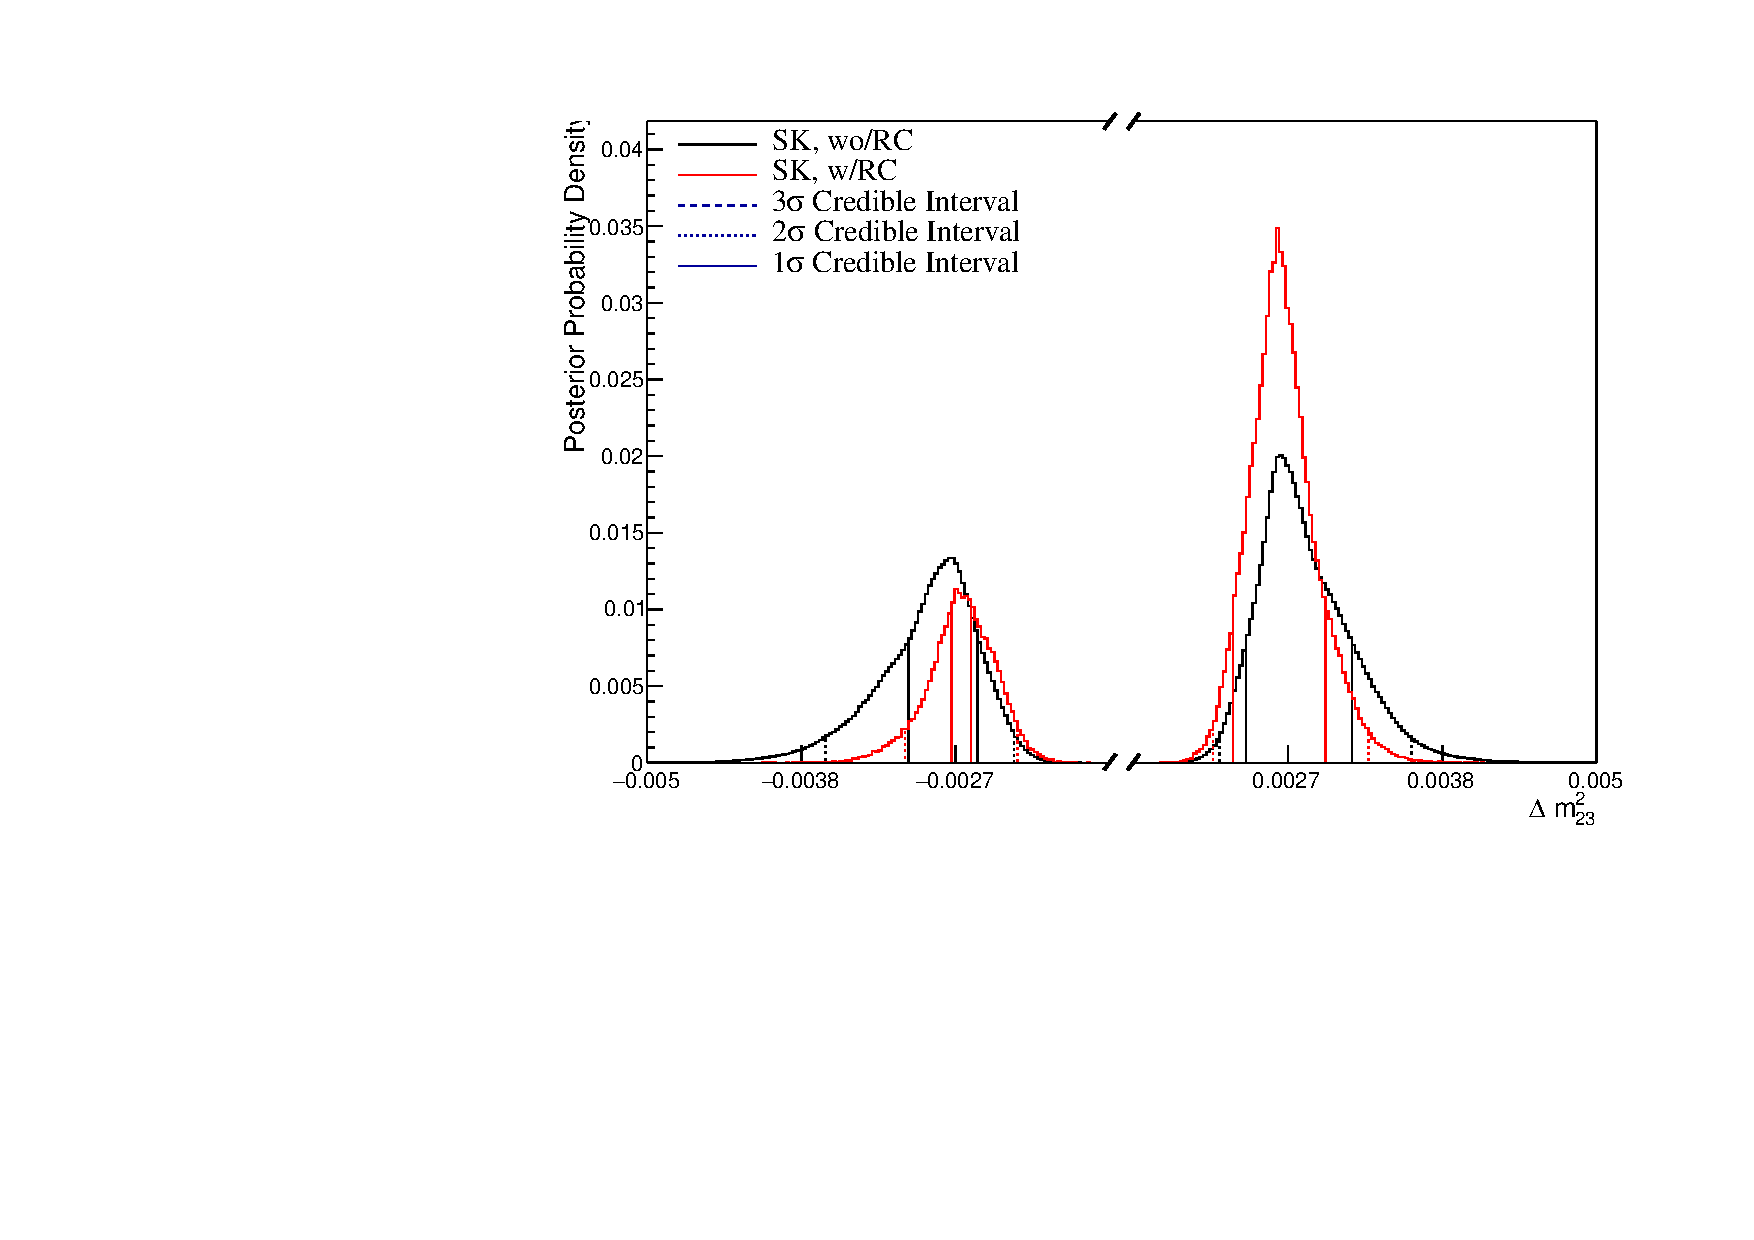
\includegraphics[width=\textwidth, trim={0mm 0mm 0mm 0mm}, clip,page=1]{Figures/OA/SKOnlyFit_wRC/ContourComparison_1D_dm32_BH_1_wRC_woRC_UnSmeared_CredibleInterval.pdf}
  \end{subfigure}
  \caption{}
  \label{fig:OscillationAnalysis_SKOnly_DELM32_WRC}
\end{figure}

The reactor constraint increases the sensitivity of the atmospheric samples to \delmsqatm as illustrated in \autoref{fig:OscillationAnalysis_SKOnly_DELM32_WRC}. Due to the marginalisation efefcts observed in \autoref{fig:OscillationAnalysis_SKOnly_TrianglePlot}, the favoured region of \delmsqatm moves closer to zero for both hierarchies. A clear explanation of this behaviour is illustrated in \autoref{fig:OscillationAnalysis_SKOnly_DELM32TH13_WRC}. The correlation between \delmsqatm and \sinsqreac is such that lower values of \sinsqreac tend towards lower values of \quickmath{|\Delta m^{2}_{32}|}. The \quickmath{1\sigma} credible interval for the \delmsqatm parameter is determined to be \quickmath{[-2.70, -2.55] \times 10^{-3} \text{eV}^{2}} and \quickmath{[2.25, 2.95] \times 10^{-3} \text{eV}^{2}}. The width of the IH credible interval is reduced by approximately \quickmath{70\%} when the reactor constraint is applied.

\begin{figure}[h]
  \begin{subfigure}[t]{1.0\textwidth}
    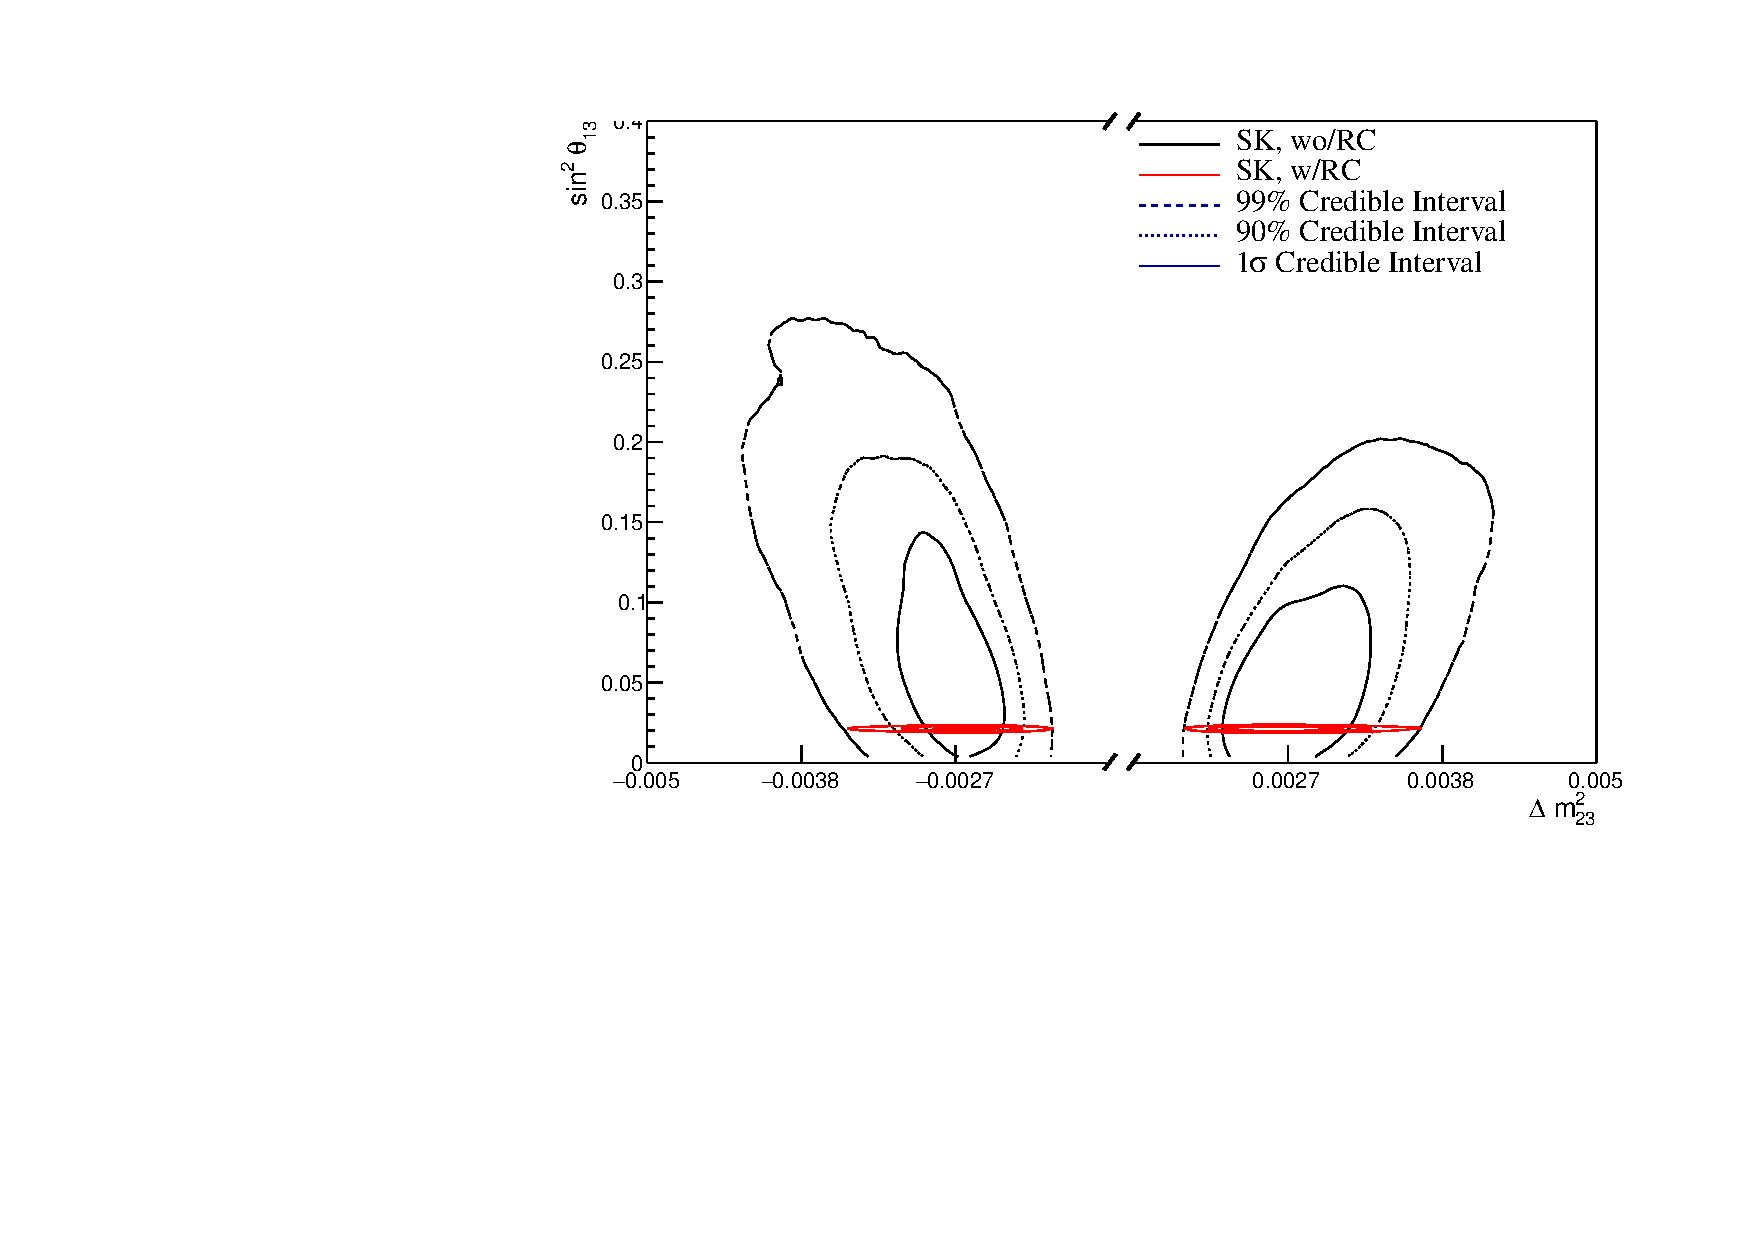
\includegraphics[width=\textwidth, trim={0mm 0mm 0mm 0mm}, clip,page=1]{Figures/OA/SKOnlyFit_wRC/ContourComparison_2D_dm32_th13_BH_0_wRC_woRC_UnSmeared_CredibleInterval.pdf}
  \end{subfigure}
  \caption{}
  \label{fig:OscillationAnalysis_SKOnly_DELM32TH13_WRC}
\end{figure}

\begin{table}[ht!]
  \centering
  \begingroup
  \renewcommand{\arraystretch}{1.5}
  \begin{tabular}{c|cc|c}
                                                        & LO \quickmath{\left(\sin^{2}\theta_{23} < 0.5 \right)} & UO \quickmath{\left( \sin^{2}\theta_{23} > 0.5 \right)} & Sum  \\ \hline
    NH \quickmath{\left( \Delta m^{2}_{32} > 0 \right)} &                                                   0.21 &                                                    0.53 & 0.74 \\
    IH \quickmath{\left( \Delta m^{2}_{32} < 0 \right)} &                                                   0.08 &                                                    0.18 & 0.26 \\ \hline
    Sum                                                 &                                                   0.29 &                                                    0.71 & 1.00 \\
  \end{tabular}
  \caption{}
  \label{tab:OscillationAnalysis_SKOnlyWRC_BayesFactors}
  \endgroup
\end{table}

The asymmetry in the number of steps within the NH to IH clearly shows that the reactor constraint increases the NH preference. The fraction of steps in each hierarchy and octant model for this fit are given in \autoref{tab:OscillationAnalysis_SKOnlyWRC_BayesFactors}. The preference of octant model is very slightly increased by the application of the reactor constraint which is consistent with expectation. The reactor constraint significantly increases the NH preference, increasing the Bayes factor from \quickmath{B(\text{NH}/\text{IH}) = 1.37} to \quickmath{B(\text{NH}/\text{IH}) = 2.85} when the reactor constraint is applied. This is still defined as a weak preference for NH according to the Jeffrey's scale (see \autoref{tab:MarkovChainMonteCarlo_JeffreysScale}), however it is a stronger preference than without the constraint. The Bayes factor for octant determination is calculated as \quickmath{B(\text{UO}/\text{LO}) = 2.45}.

\subsection{Application of Near Detector Constraints for Atmospheric Samples}
\label{sec:OscillationAnalysis_SKOnly_NoND}

The choice to apply the near detector constraints onto the low energy atmospheric samples was introduced in \autoref{sec:SelsAndSysts_Systs_Interaction}. The effect of this choice can be studied by comparing the sensitivities of the atmospheric only analysis when the near detector constraints are and are not applied. The change in sensitivity on \dcp is given in \autoref{fig:OscillationAnalysis_SKOnly_NoND_DCP}. The shape of the posterior is approximately the same although slightly less peaked at the asimov point. The width of the \quickmath{1\sigma} credible intervals are approximately the same (identical to within a bin width) and the same conclusion holds for the higher credible intervals. Similar conclusions hold for the other oscillation parameters. As expected, the sensitivities are still statistics dominated and the exact choice of systematic model and constraint does not effect the physics conclusions one would make from this analysis.

\begin{figure}[h]
  \begin{subfigure}[t]{1.0\textwidth}
    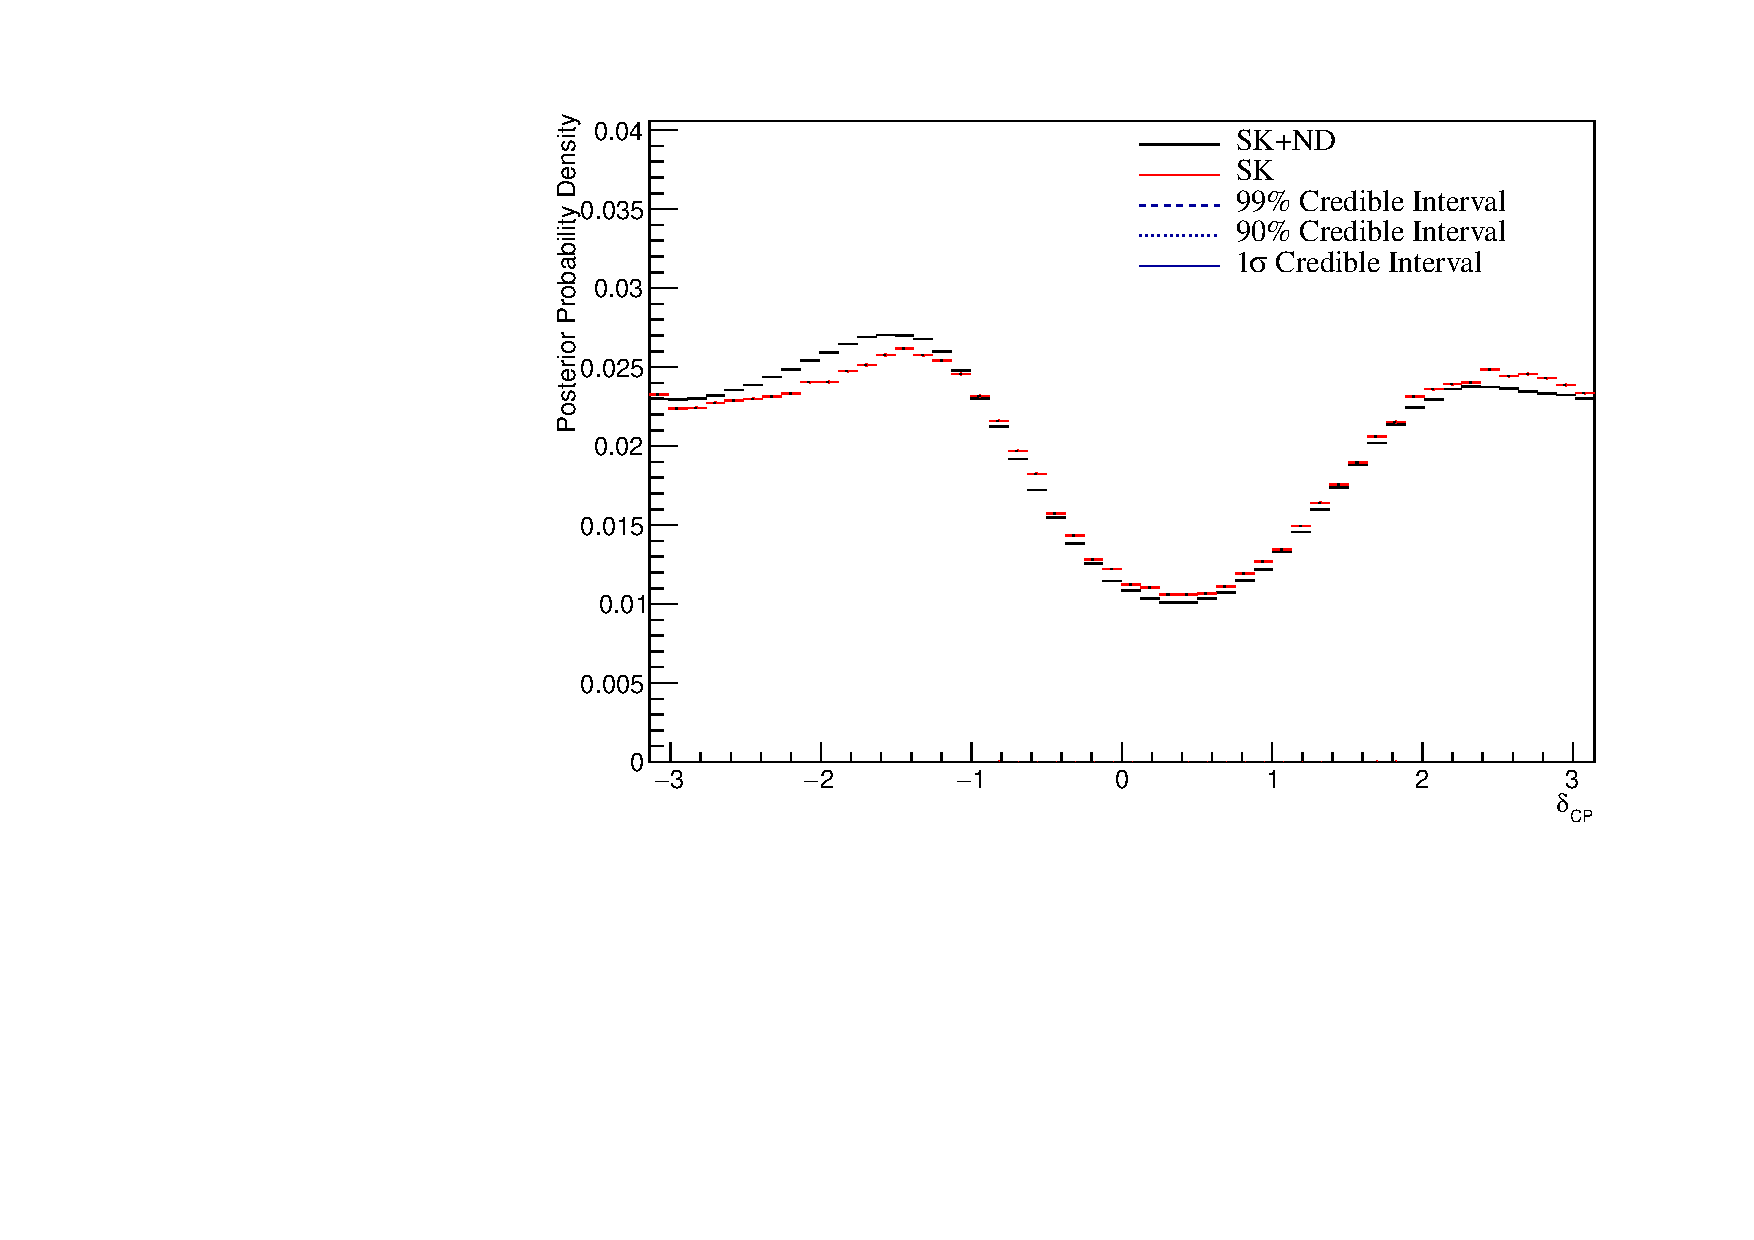
\includegraphics[width=\textwidth, trim={0mm 0mm 0mm 0mm}, clip,page=1]{Figures/OA/SKOnlyFit_noND/ContourComparison_1D_dcp_BH_0_woRC_UnSmeared_CredibleInterval.pdf}
  \end{subfigure}
  \caption{}
  \label{fig:OscillationAnalysis_SKOnly_NoND_DCP}
\end{figure}

\subsection{Atmospheric and Beam Sensitivity without Reactor Constraint}
\label{sec:OscillationAnalysis_JointFit}

This section presents the sensitivities of the simulataneous beam and atmospheric analysis without the reactor constraint. The asimov data is built assuming the post-BANFF cross section tune and Asimov A oscillation parameters defined in \autoref{tab:Theory_ParameterSets}. This is a fit to all 18 near detector beam samples, 5 far detector beam samples and 18 atmospheric samples. The sensitivity to \dcp, marginalised over both hierarchies is given in \autoref{fig:OscillationAnalysis_JointFit_DCP}.

\begin{figure}[h]
  \begin{subfigure}[t]{1.0\textwidth}
    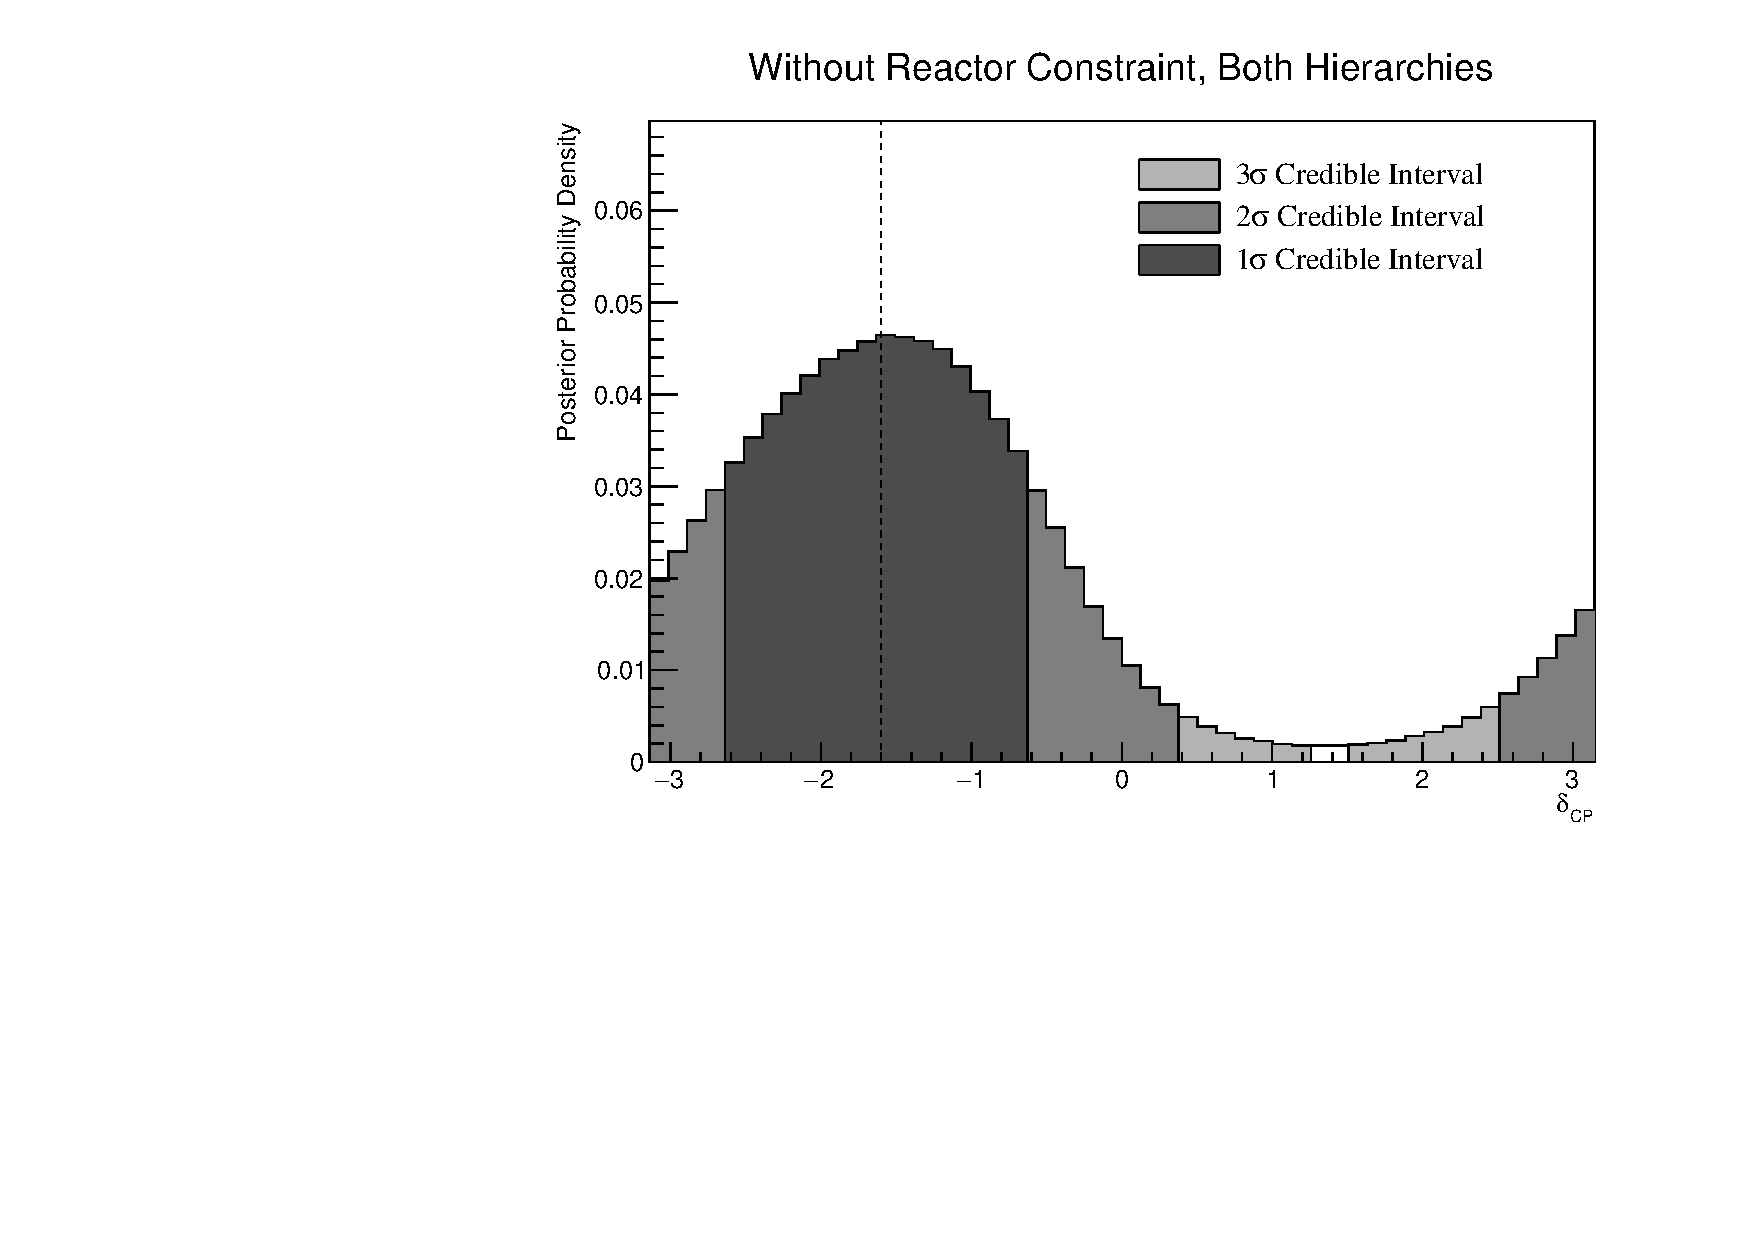
\includegraphics[width=\textwidth, trim={0mm 0mm 0mm 0mm}, clip,page=1]{Figures/OA/JointFit/Contours_1D_dcp_BH_1_woRC_UnSmeared_CredibleInterval.pdf}
  \end{subfigure}
  \caption{}
  \label{fig:OscillationAnalysis_JointFit_DCP}
\end{figure}

The credible intervals and highest posterior distribution for each oscillation parameter is given in \autoref{tab:OscillationAnalysis_JointFit_CredIntervals}. The highest posterior density is \quickmath{\delta_{CP} = -1.58} and is clearly compatible with the known Asimov A value of \quickmath{\delta_{CP} = -1.601}. The CP-conserving values of \quickmath{\delta_{CP}=0, \pi, -\pi} are disfavoured at \quickmath{1\sigma} credible interval. There is also a region around \quickmath{\delta_{CP} = 1.4} which is disfavoured at more than \quickmath{3\sigma}. Whilst these conclusions can be made at this particular asimov point, it does show that if the true value of \quickmath{\delta_{CP}} was CP-violating, this joint analysis would be able to disfavour CP conserving values at over \quickmath{1\sigma}. The highest posterior density does move further away from the asimov point when only steps in the NH region are considered. This is due to the correlations between the value of \dcp and the mass hierarchy. 

\begin{table}[ht!]
  \centering
  \begingroup
  \renewcommand{\arraystretch}{1.5}
  \begin{tabular}{c|c|c}
    Parameter               & Interval & HPD \\ \hline
    \quickmath{\delta_{CP}, \text{ (BH)}} & \quickmath{\left[ -2.64, -0.63 \right]} & -1.57 \\
    \quickmath{\delta_{CP}, \text{ (NH)}} & \quickmath{\left[ -2.76, -0.63 \right]} & -1.45 \\
    \quickmath{\delta_{CP}, \text{ (IH)}} & \quickmath{\left[ -2.39, -0.88 \right]} & -1.57 \\ \hline
    \quickmath{\Delta m^{2}_{32} \text{ (BH) } [\times 10^{-3} \text{eV}^{2}]} & \quickmath{\left[ 2.46, 2.58 \right]} & 2.49 \\
    \quickmath{\Delta m^{2}_{32} \text{ (NH) } [\times 10^{-3} \text{eV}^{2}]} & \quickmath{\left[ 2.48, 2.56 \right]} & 2.51 \\
    \quickmath{\Delta m^{2}_{32} \text{ (IH) } [\times 10^{-3} \text{eV}^{2}]} & \quickmath{\left[ -2.60, -2.52 \right]} & -2.55 \\ \hline
    \quickmath{\sin^{2}(\theta_{23}) \text{ (BH) }} & \quickmath{\left[ 0.48, 0.55 \right]} & 0.509 \\ 
    \quickmath{\sin^{2}(\theta_{23}) \text{ (NH) }} & \quickmath{\left[ 0.48, 0.55 \right]} & 0.509 \\ 
    \quickmath{\sin^{2}(\theta_{23}) \text{ (IH) }} & \quickmath{\left[ 0.48, 0.55 \right]} & 0.521 \\ \hline \hline
  \end{tabular}
  \caption{}
  \label{tab:OscillationAnalysis_JointFit_CredIntervals}
  \endgroup
\end{table}

The sensitivity to \delmsqatm is illustrated in \autoref{fig:OscillationAnalysis_JointFit_DCP} for the normal hierarchy model hypotheses. Notably, the \quickmath{1\sigma} credible interval is entirely contained within the normal hierarchy region, as illustrated in \autoref{tab:OscillationAnalysis_JointFit_CredIntervals}. This is illustrates reasonable sensitivity to the mass hierarchy model. This is also reflected in the \quickmath{1\sigma} credible intervals being approximately the same when they are made considering both hierarchies and when considering only the NH.

The fraction of steps in each of the mass hierarchy regions and octants of \sinsqatm is given in \autoref{tab:OscillationAnalysis_JointFit_BayesFactors}. The Bayes factors are determined to be \quickmath{B(\text{NH}/\text{IH}) = 3.67} and \quickmath{B(\text{UO}/\text{LO}) = 1.73}. Jeffrey's scale (presented in \autoref{tab:MarkovChainMonteCarlo_JeffreysScale}) states that this value of the hierarchy Bayes factor illustrates suubstantial evidence for normal hierarchy. This corresponds the known oscillation parameters input into the asimov data and is a strong statement than the  atmospheric-only analysis can provide. The Bayes factor for octant determination represents a weak preference for the upper octant.

\begin{table}[ht!]
  \centering
  \begingroup
  \renewcommand{\arraystretch}{1.5}
  \begin{tabular}{c|cc|c}
                                                        & LO \quickmath{\left(\sin^{2}\theta_{23} < 0.5 \right)} & UO \quickmath{\left( \sin^{2}\theta_{23} > 0.5 \right)} & Sum  \\ \hline
    NH \quickmath{\left( \Delta m^{2}_{32} > 0 \right)} &                                                   0.29 &                                                    0.50 & 0.79 \\
    IH \quickmath{\left( \Delta m^{2}_{32} < 0 \right)} &                                                   0.08 &                                                    0.13 & 0.21 \\ \hline
    Sum                                                 &                                                   0.37 &                                                    0.63 & 1.00 \\
  \end{tabular}
  \caption{}
  \label{tab:OscillationAnalysis_JointFit_BayesFactors}
  \endgroup
\end{table}

The Asimov A definition is \quickmath{\Delta m^{2}_{32} = 2.509 \times 10 ^{-3} \text{eV}^{2}}. The normal hierarchy distribution clearly favours this region with the highest posterior density of \quickmath{\Delta m^{2}_{32} = 2.51 \times 10 ^{-3} \text{eV}^{2}}. The highest posterior density contained within the inverse hierarchy posterior distribution is \quickmath{\Delta m^{2}_{32} = -2.55 \times 10 ^{-3} \text{eV}^{2}}.

\begin{figure}[h]
  \begin{subfigure}[t]{1.0\textwidth}
    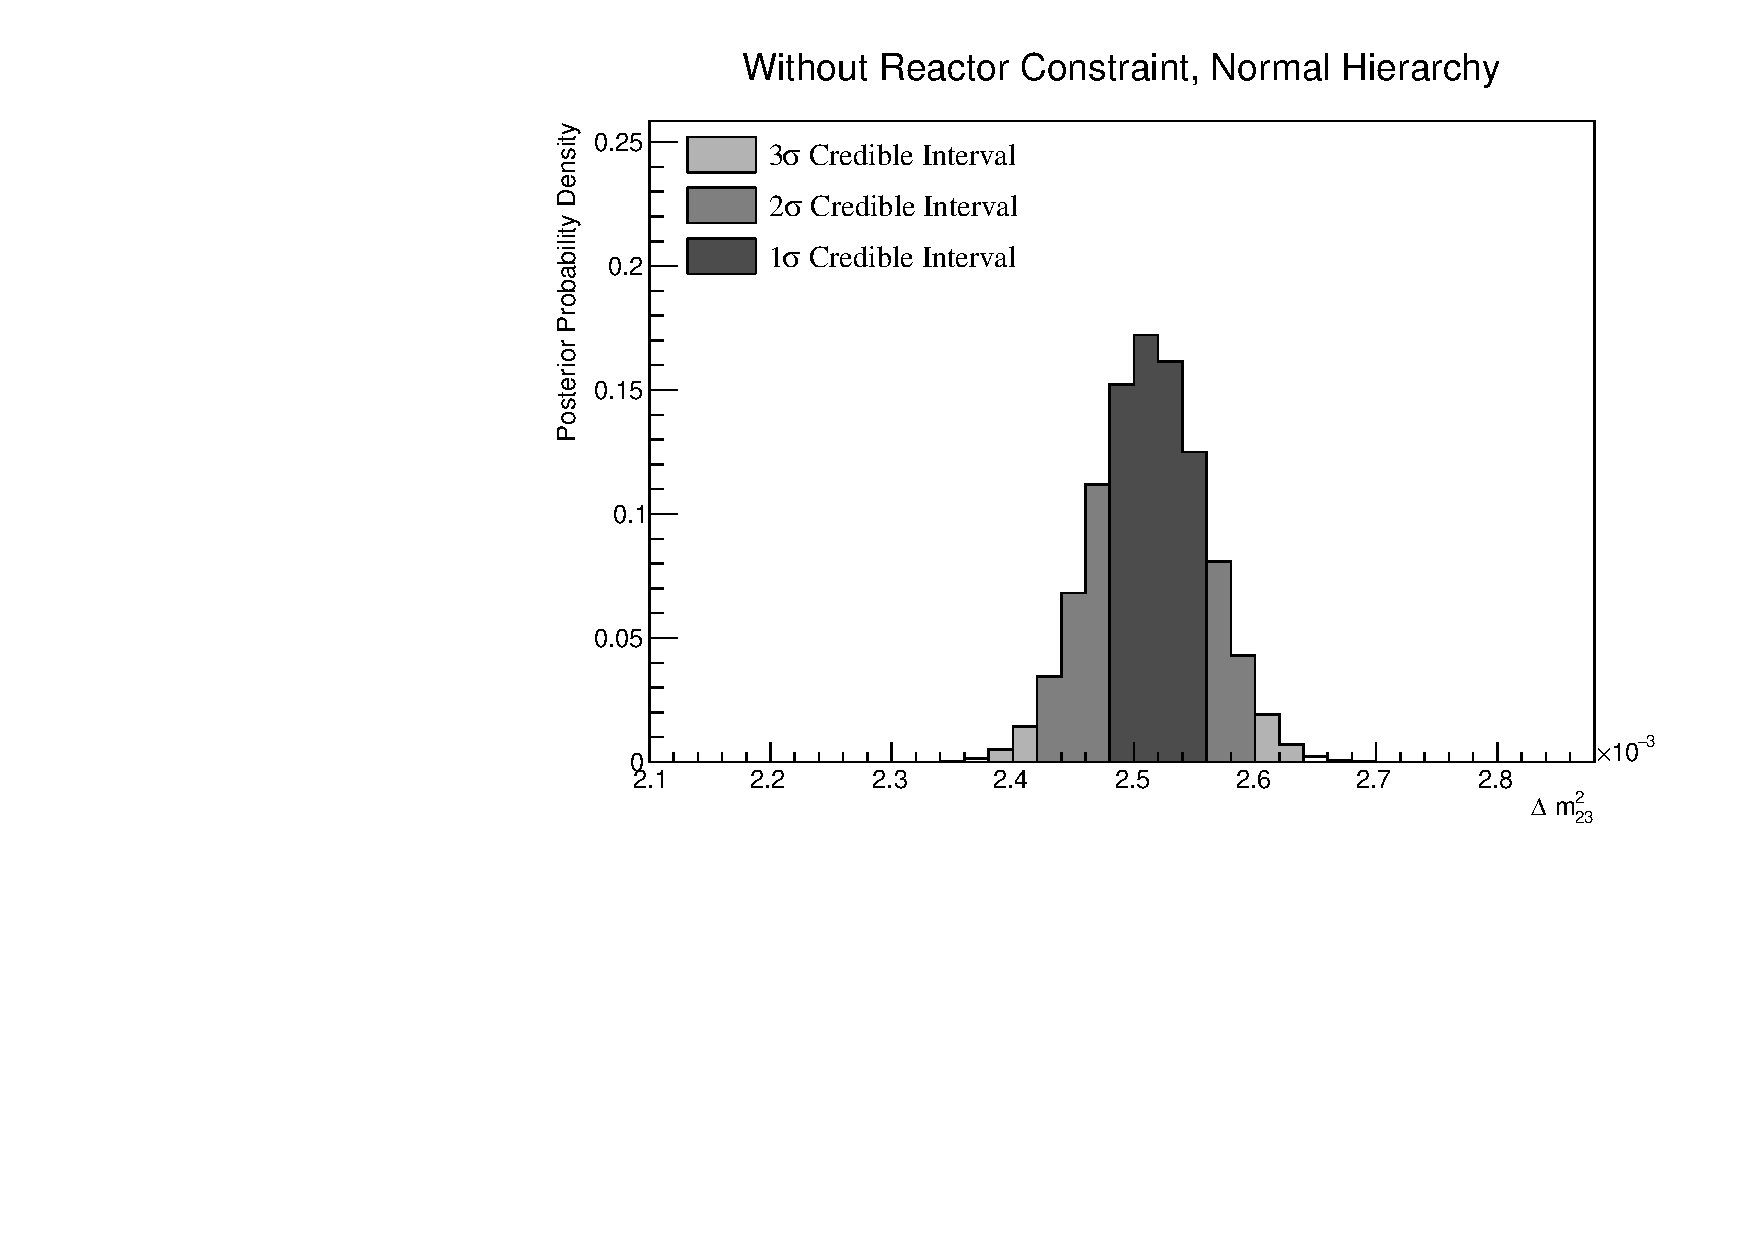
\includegraphics[width=\textwidth, trim={0mm 0mm 0mm 0mm}, clip,page=1]{Figures/OA/JointFit/Contours_1D_dm32_NH_1_woRC_UnSmeared_CredibleInterval.pdf}
  \end{subfigure}
  \caption{}
  \label{fig:OscillationAnalysis_JointFit_DELM32}
\end{figure}

The sensitivity to \sinsqatm is presented in \autoref{fig:OscillationAnalysis_JointFit_TH23}. There is clear preference for the upper octant but the peak of the distribution is relatively flat. It peaks in the region of the expected Asimov value of \quickmath{\sin^{2}(\theta_{23}) = 0.528}. The difference in the highest posterior distribution and the width of the credible interval is relatively unchanged when considering different hierarchy models. Consequently, the correlation between \delmsqatm and \sinsqatm is such that it is approximately mirrored across the hierarchy discontinuity.

\begin{figure}[h]
  \begin{subfigure}[t]{1.0\textwidth}
    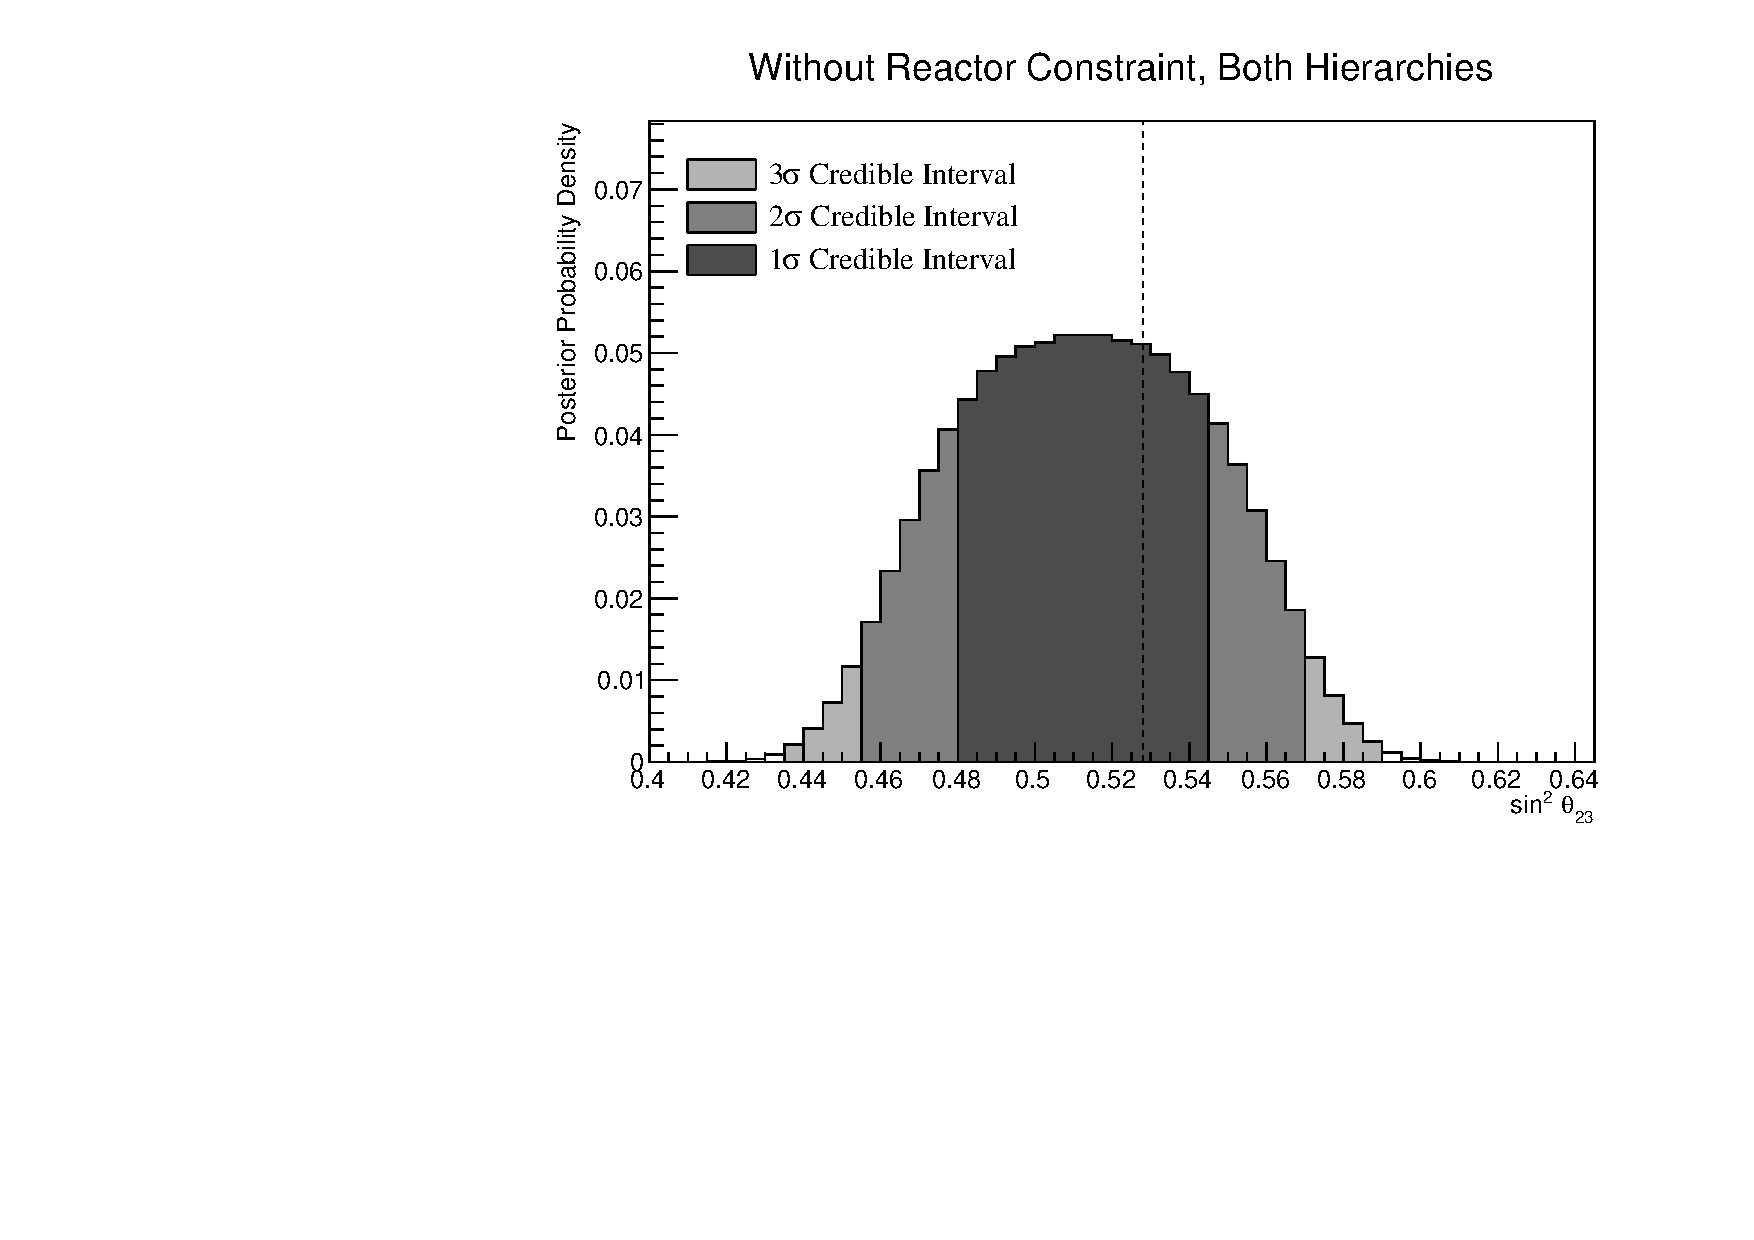
\includegraphics[width=\textwidth, trim={0mm 0mm 0mm 0mm}, clip,page=1]{Figures/OA/JointFit/Contours_1D_th23_BH_1_woRC_UnSmeared_CredibleInterval.pdf}
  \end{subfigure}
  \caption{}
  \label{fig:OscillationAnalysis_JointFit_TH23}
\end{figure}

The sensitivity presented as a function of the appearance parameters (\quickmath{\sin^{2}(\theta_{13}) - \delta_{CP}}) is given in \autoref{fig:OscillationAnalysis_JointFit_DCPTH13}. As expected, the contours follow that given in \autoref{fig:OscillationAnalysis_2DLLHOscScans_App}, where the \quickmath{2\sigma} credible intervals have a closed contour excluding the region around \quickmath{\delta_{CP} \sim 1.2}. The width of the \quickmath{3\sigma} credible interval is also clearly dependent upon the value of \quickmath{\delta_{CP}}. Close to the asimov point, \quickmath{\delta_{CP} = -1.601}, the width of the \quickmath{3\sigma} credible interval approximately spans \quickmath{\sin^{2}(\theta_{13}) = [0.013, 0.04]}. This is reduced to a region of \quickmath{\sin^{2}(\theta_{13}) = [0.023, 0.042]} at the most disfavour value of \quickmath{\delta_{CP}}. The \quickmath{1\sigma} credible interval is consistent with both the asimov point and the reactor constraint. Application of the reactor constraint would be expected to decreased the  width of the \quickmath{1\sigma} credible intervals of \dcp due to the triangular shape of the posterior probability. 

The sensitivity in terms of the `disappearance' parameters marginalised over both hierarchies is given in \autoref{fig:OscillationAnalysis_JointFit_DM32TH23}. In this two-dimensional projection of the posterior distribution, a small section of the \quickmath{1\sigma} credible interval is contained within the inverse hierarchy region. That IH region is clearly favouring the upper octant as expected. The \quickmath{1\sigma} credible region of the NH contour spans both octants but favours the UO.

\begin{figure}[h]
  \begin{subfigure}[t]{0.95\textwidth}
    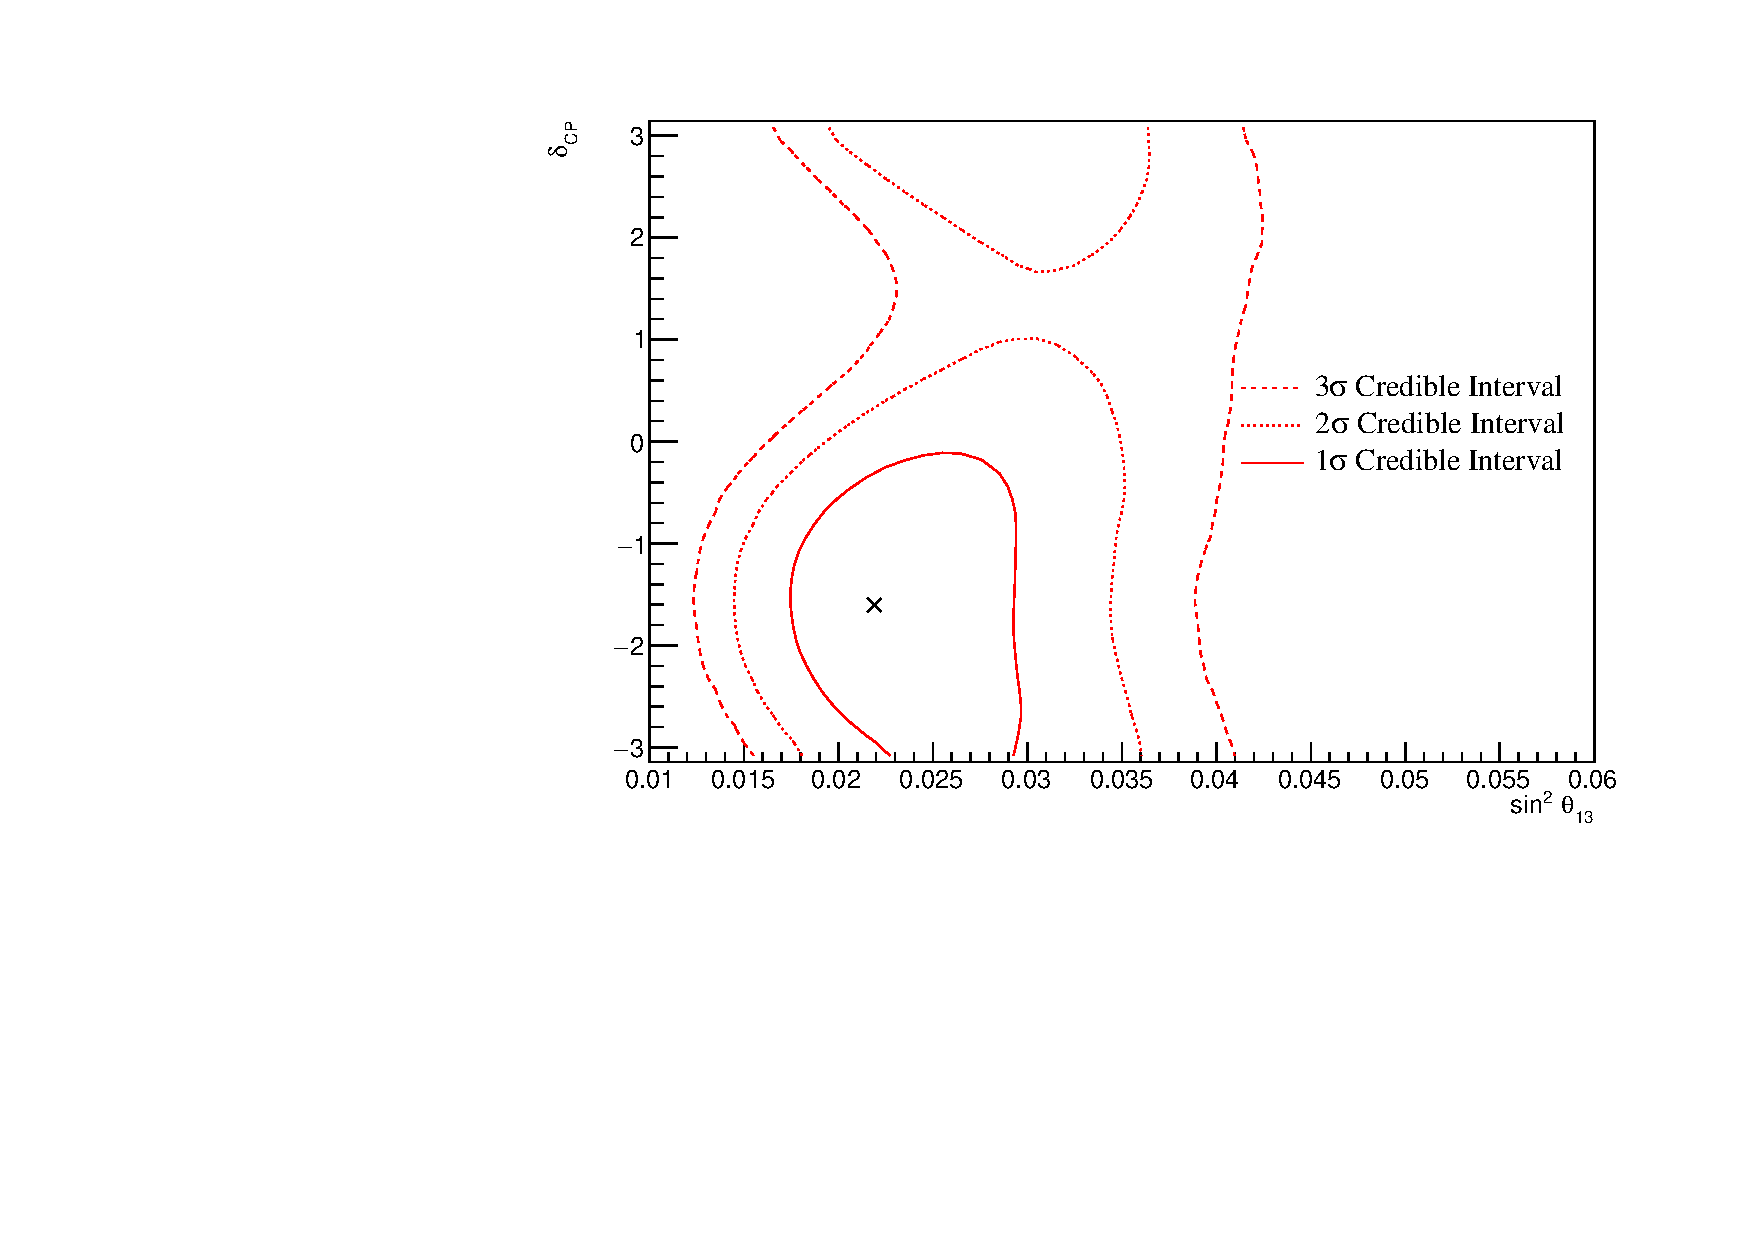
\includegraphics[width=\textwidth, trim={0mm 0mm 0mm 0mm}, clip,page=1]{Figures/OA/JointFit/Contours_2D_th13_dcp_BH_1_woRC_UnSmeared_CredibleInterval.pdf}
  \end{subfigure}
  \caption{}
  \label{fig:OscillationAnalysis_JointFit_DCPTH13}
\end{figure}

\begin{figure}[h]
  \begin{subfigure}[t]{0.95\textwidth}
    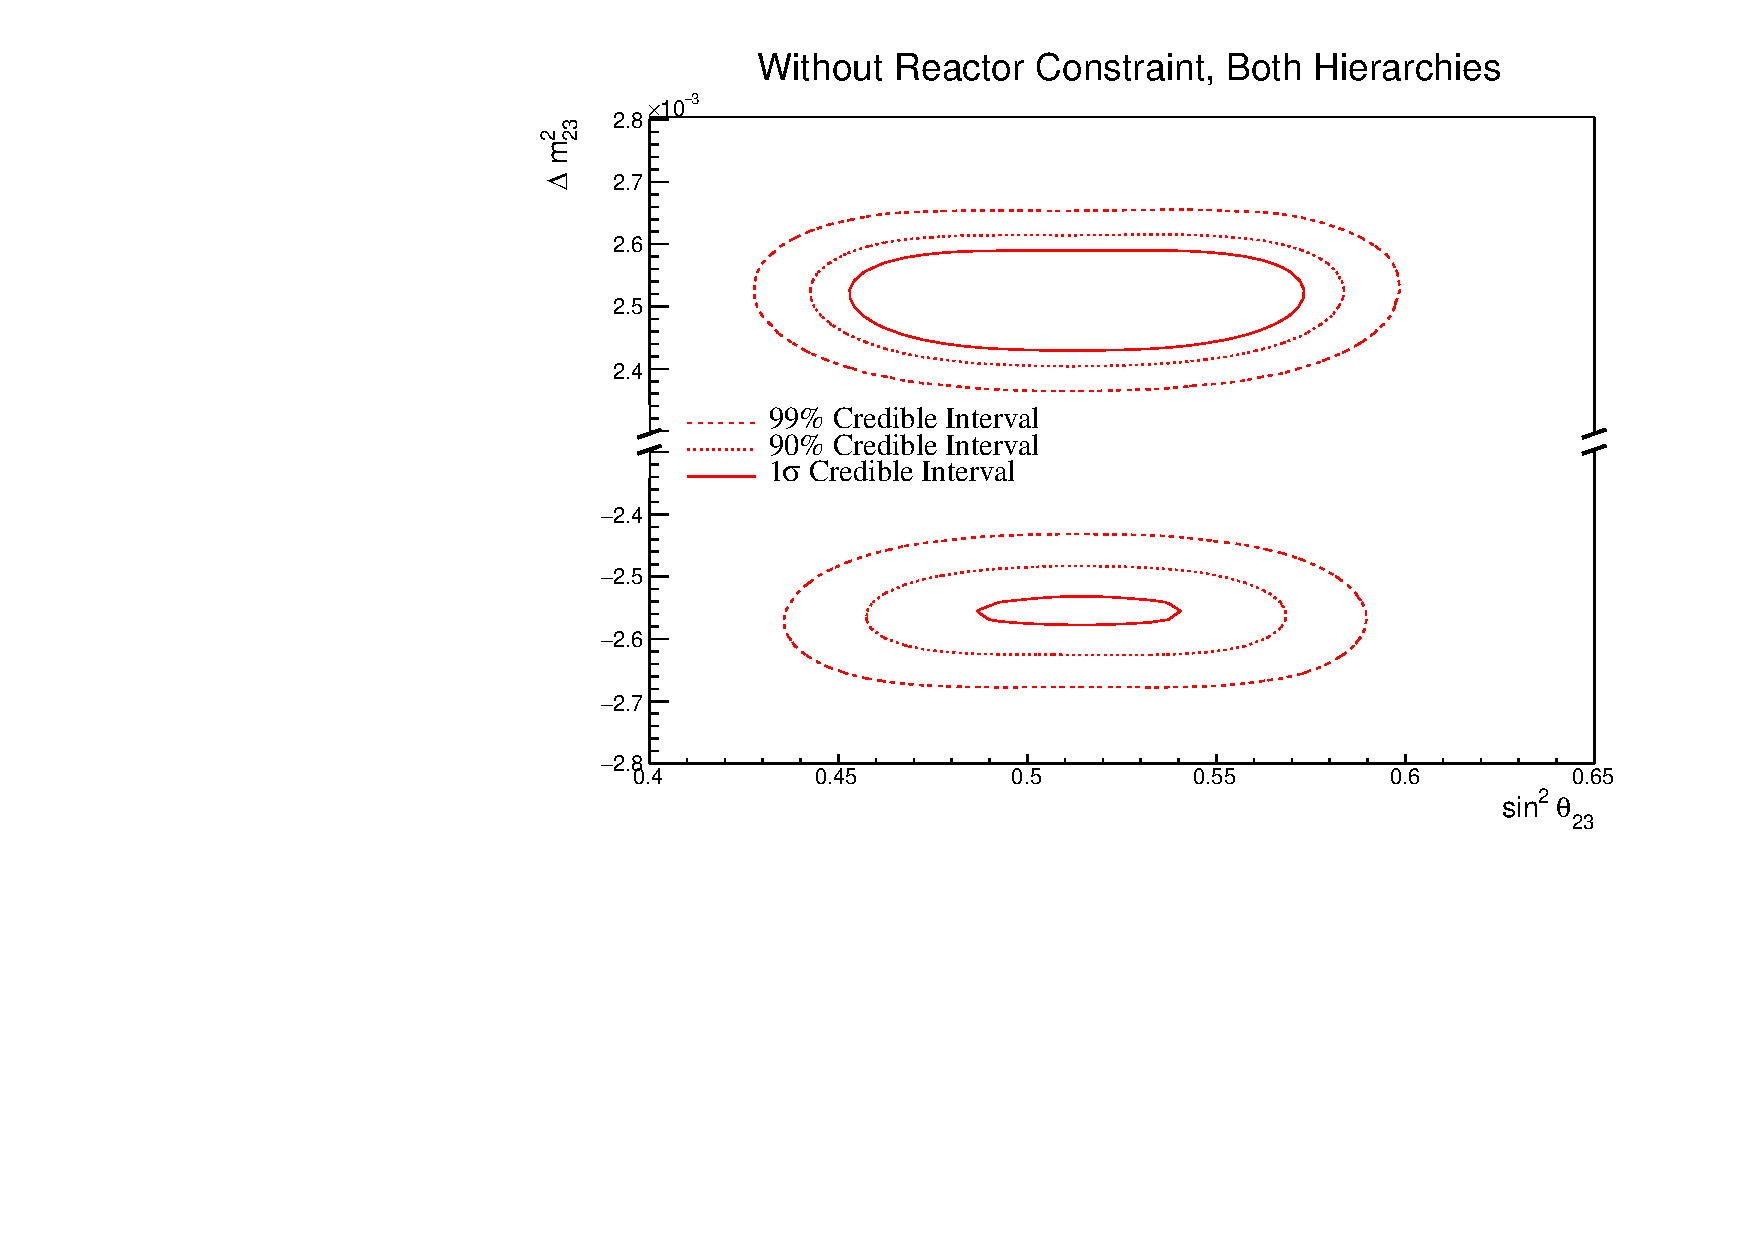
\includegraphics[width=\textwidth, trim={0mm 0mm 0mm 0mm}, clip,page=1]{Figures/OA/JointFit/Contours_2D_th23_dm32_BH_0_woRC_UnSmeared_CredibleInterval.pdf}
  \end{subfigure}
  \caption{}
  \label{fig:OscillationAnalysis_JointFit_DM32TH23}
\end{figure}

\clearpage

The two-dimensional posterior distribution for each permutation of the oscillaton parameters of interest is given in \autoref{fig:OscillationAnalysis_JointFit_TriPlot}. The most notable observation is that the \sinsqreac and \sinsqatm are anti-correlated. If the value of \sinsqreac was known to be closer to the asimov point, the preferred value of \sinsqatm would increase. That would move the highest posterior probability closer in line with the asimov value. This also means that, the preference for the UO would be increased if the reactor constraint was to be applied. 

\begin{figure}[h]
  \begin{subfigure}[t]{1.0\textwidth}
    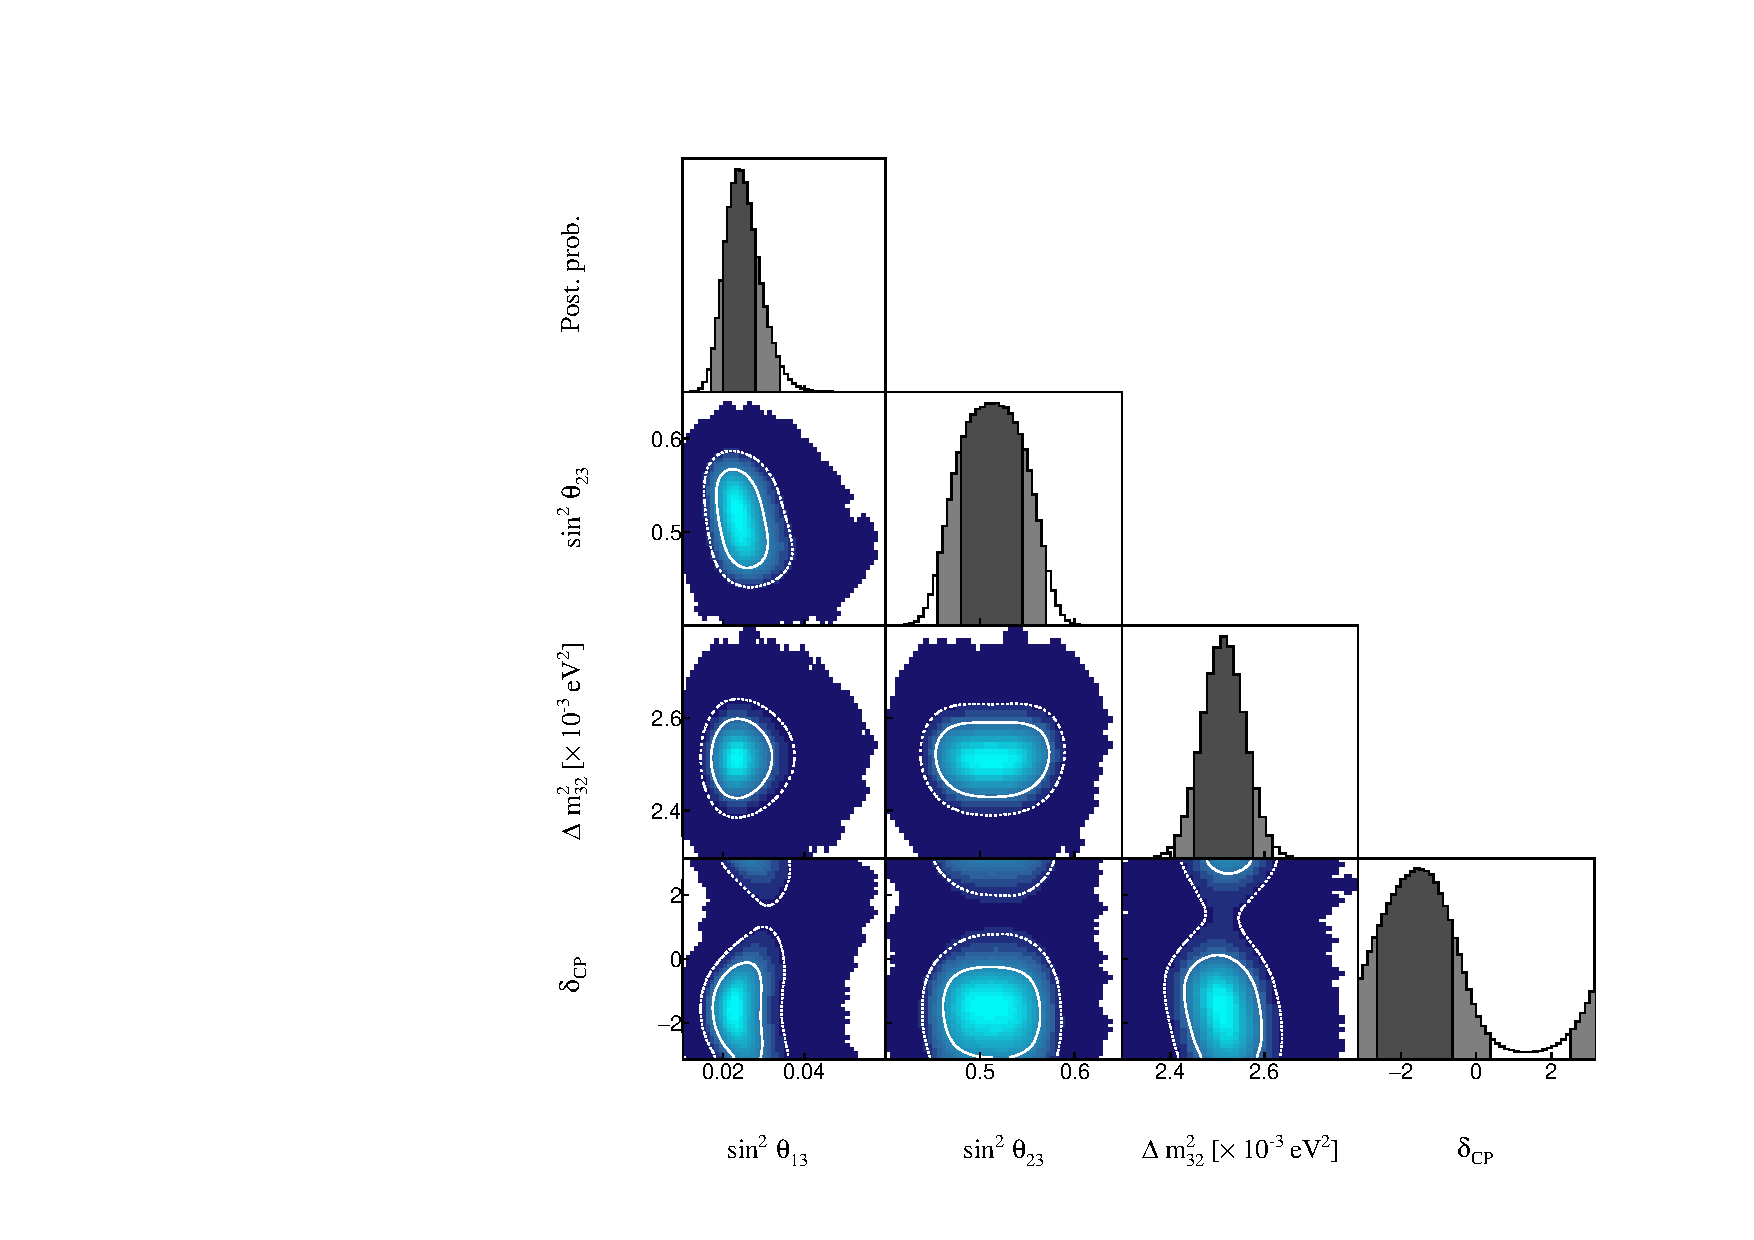
\includegraphics[width=\textwidth, trim={0mm 0mm 0mm 0mm}, clip,page=1]{Figures/OA/JointFit/Contours_1D_woRC_UnSmeared_CredibleInterval_TrianglePlot.pdf}
  \end{subfigure}
  \caption{}
  \label{fig:OscillationAnalysis_JointFit_TriPlot}
\end{figure}

The correlation between \sinsqreac and \delmsqatm can be seen in \autoref{fig:OscillationAnalysis_JointFit_DM32TH13}. A much larger fraction of the posterior distribution is contained in the NH for lower values of \sinsqreac. Consequently, the application of the reactor constraint would be expected to signficantly increase the preference for NH.

\begin{figure}[h]
  \begin{subfigure}[t]{1.0\textwidth}
    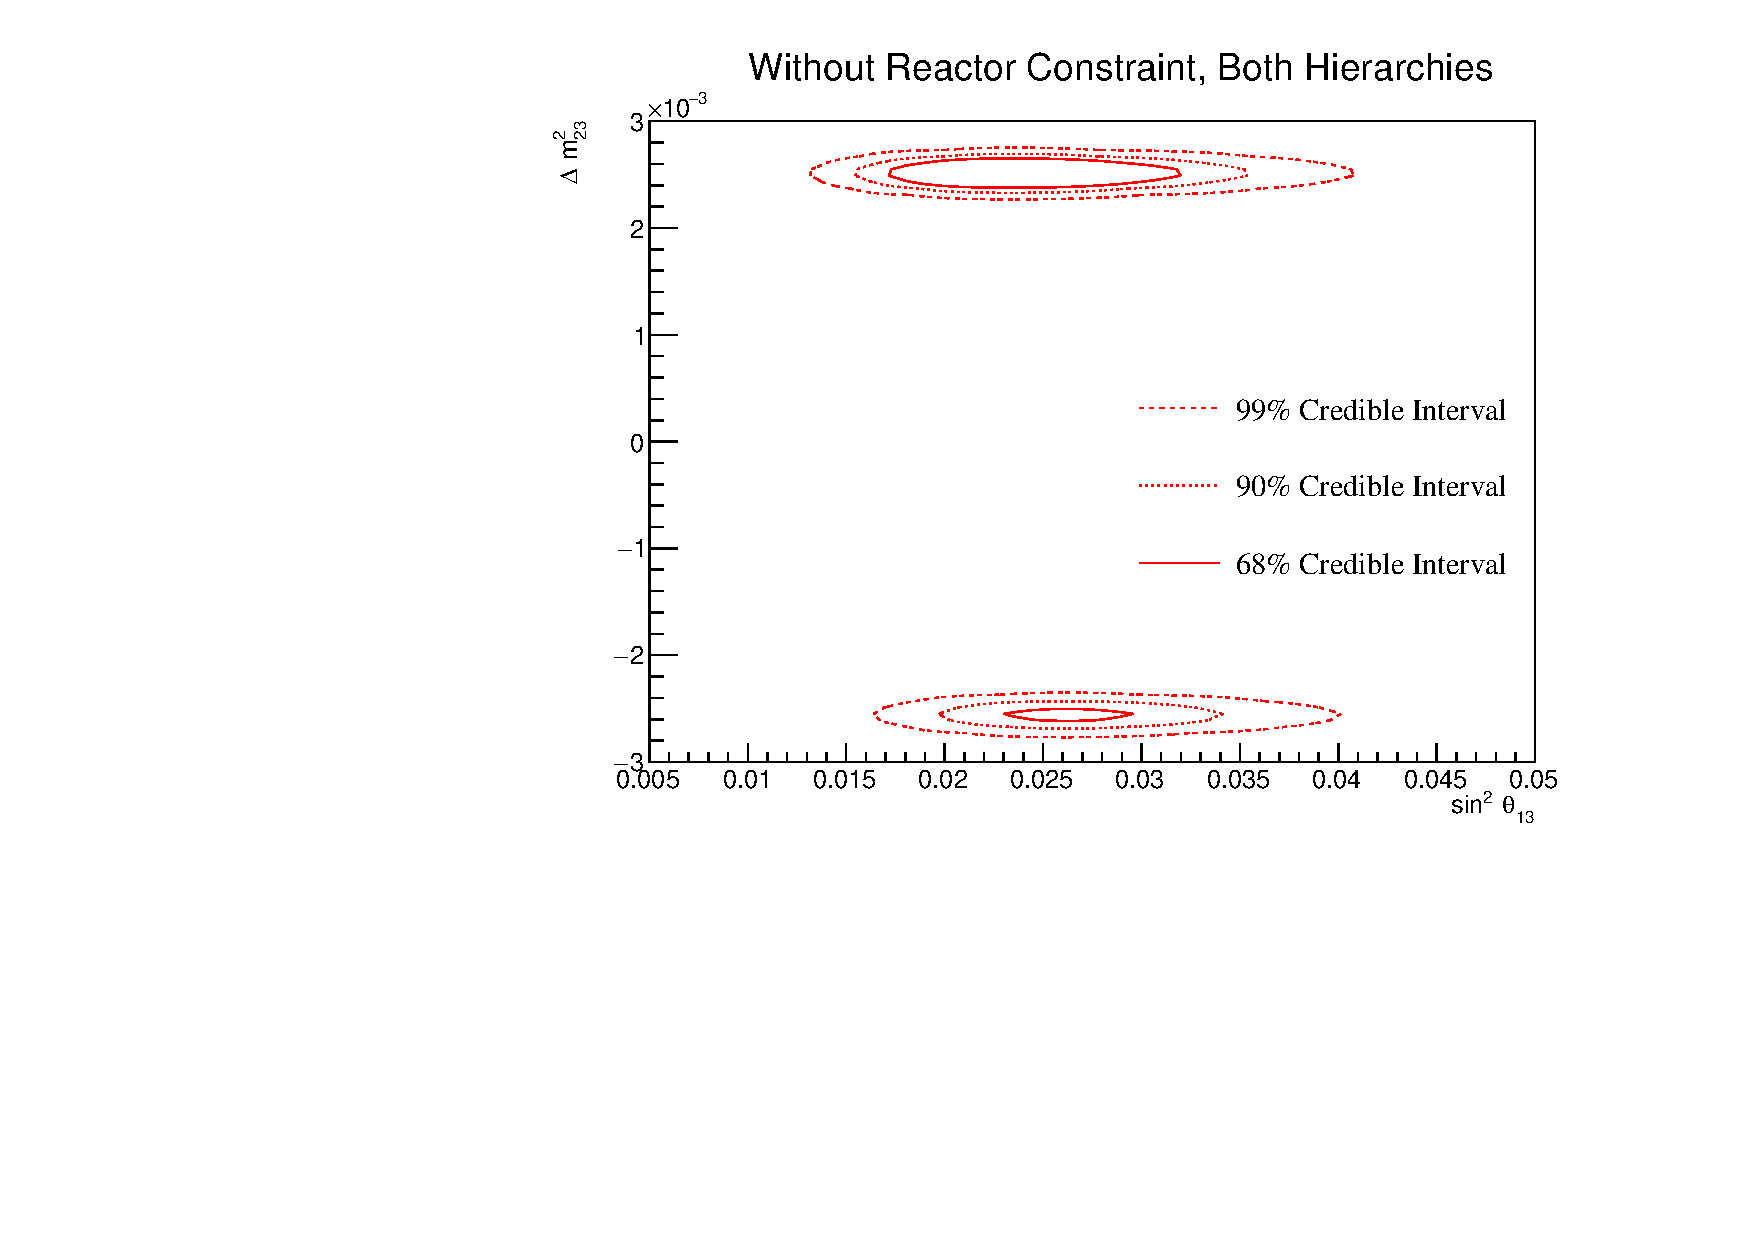
\includegraphics[width=\textwidth, trim={0mm 0mm 0mm 0mm}, clip,page=1]{Figures/OA/JointFit/Contours_2D_th13_dm32_BH_0_woRC_UnSmeared_CredibleInterval.pdf}
  \end{subfigure}
  \caption{}
  \label{fig:OscillationAnalysis_JointFit_DM32TH13}
\end{figure}

\subsection{Atmospheric and Beam Sensitivity with Reactor Constraint}
\label{sec:OscillationAnalysis_JointFit_wRC}



\subsection{Comparison to Latest T2K Sensitivities}

